\documentclass[12pt]{report}
\usepackage{etex}
\usepackage[margin=1in]{geometry}

\usepackage{amsmath,mathrsfs, enumerate,amsthm}
\usepackage{mathtools,bbm}
\usepackage{amssymb}
\usepackage{pstricks,pst-plot,psfrag}
\usepackage[all]{xy}
\usepackage{graphicx,wrapfig,subfigure,xspace,bm}
% Commands for algorithms
%\usepackage{algorithm,algorithmic}
\usepackage[lined,linesnumbered,algoruled,noend]{algorithm2e}
\usepackage{pgfgantt}
\usepackage[]{algorithm2e}
\usepackage{gensymb}
\usepackage{bigints}

\usepackage{hyperref}
\hypersetup{
    colorlinks,
    citecolor=black,
    filecolor=black,
    linkcolor=black,
    urlcolor=black
}
%\usepackage[utf8]{inputenc}
%\usepackage[english]{babel}

\newtheorem{theorem}{Theorem}[section]
\newtheorem{definition}[theorem]{Definition}
\newtheorem{assumption}[theorem]{Assumption}
\newtheorem{lemma}[theorem]{Lemma}
\newtheorem{claim}[theorem]{Claim}
\newtheorem{remarks}[theorem]{Remarks}
\newtheorem{remark}[theorem]{Remark}
\newtheorem{example}[theorem]{Example}
\newtheorem{corollary}[theorem]{Corollary}
\newtheorem{proposition}[theorem]{Proposition}  

\newcommand\bah[1]{\textcolor{blue}{#1}}
\newcommand\drew[1]{\textcolor{red}{#1}}

%%%
\newcommand\subscr[2]{#1_{\textup{#2}}}
\newcommand\upscr[2]{#1^{\textup{#2}}}
\newcommand\upsubscr[3]{#1_{\textup{#2}}^{\textup{#3}}}
%%%%

\newcommand{\todo}[1]{\par\noindent{\color{magenta}
    \raggedright\textsc{#1}\par\marginpar{\Large $\star$}}}

\newcommand{\din}{\subscr{d}{in}}
\newcommand{\wdin}{\upsubscr{d}{in}{w}}
\newcommand{\dout}{\subscr{d}{out}}
\newcommand{\wdout}{\upsubscr{d}{out}{w}}
\newcommand{\wdoutmax}{\upsubscr{d}{out,max}{w}}
%\newcommand{\rank}[3]{\mathrm{rank}(#1, \pref{#2}{#3})}
\newcommand{\rank}{\mathrm{rank}}
\newcommand{\Nin}{\upscr{\mathcal{N}}{in}}
\newcommand{\Nout}{\upscr{\mathcal{N}}{out}}
\newcommand{\wdegree}{\upsubscr{d}{}{w}}
\renewcommand{\SS}{\switch_{\text{agree}}}
\newcommand{\WW}{\mathcal{W}}
\newcommand{\Norm}[1]{\|#1\|}
\newcommand{\TwoNorm}[1]{\|#1\|_2}
\newcommand{\OneNorm}[1]{\|#1\|_1}

% Change numbering to Roman numerals
\renewcommand\thesection{\Roman{section}}
\renewcommand\thesubsection{\arabic{section}.\arabic{subsection}}
\renewcommand\thedefinition{\arabic{section}.\arabic{definition}}
\renewcommand\thetheorem{\arabic{section}.\arabic{theorem}}

%% Math defs
\newcommand{\argmax}{\mathrm{argmax}}

% complex
\newcommand{\realpart}{\mathrm{Re}}
\newcommand{\impart}{\mathrm{Im}}

\newcommand{\real}{{\mathbb{R}}}
\newcommand{\realpositive}{{\mathbb{R}}_{>0}}
\newcommand{\realnonnegative}{{\mathbb{R}}_{\ge 0}}
\newcommand{\integers}{\mathbb{Z}}
\newcommand{\integerspositive}{\mathbb{Z}_{\geq 1}}
\newcommand{\integersnonnegative}{\mathbb{Z}_{\geq 0}}
\newcommand{\eps}{\epsilon}
\newcommand{\argmin}{\operatorname{argmin}}
\newcommand{\until}[1]{\{1,\dots,#1\}}
\newcommand{\map}[3]{#1:#2 \rightarrow #3}
\newcommand{\setmap}[3]{#1:#2 \rightrightarrows #3}
\newcommand{\equilibria}[1]{\operatorname{Eq}(#1)}
\newcommand{\pder}[2]{\frac{\partial #1}{\partial #2}}
\newcommand{\pdertwo}[2]{\frac{\partial^2 #1}{\partial #2^2}}
\newcommand{\pdertwom}[3]{\frac{\partial^2 #1}{\partial #2\partial #3}}

% Drew's commands--------------------
\newcommand{\V}{\mathcal{V}}
\newcommand{\E}{\mathcal{E}}
\newcommand{\M}{\mathcal{M}}
\newcommand{\thetadot}{\dot{\theta}}
\newcommand{\complex}{\mathbb{C}}
%Indent enumerate
\newcommand{\indentitem}{\setlength\itemindent{25pt}} 
%---------------------------------------------

\newcommand{\oprocendsymbol}{\hbox{$\bullet$}}
\newcommand{\oprocend}{\relax\ifmmode\else\unskip\hfill\fi\oprocendsymbol}
\def\eqoprocend{\tag*{$\bullet$}}
\newcommand{\longthmtitle}[1]{\mbox{}\textup{\textbf{(#1)}}}

\newcommand{\margin}[1]{\marginpar{\color{red}\tiny\ttfamily#1}}
\newcommand{\marginb}[1]{\marginpar{\color{blue}\tiny\ttfamily#1}}
\newcommand{\killedb}[1]{\marginpar{\color{black}\tiny\ttfamily#1}}
\newcommand{\comment}[1]{\par\noindent{\raggedright\textsf{\color{blue}
      #1}\par\marginpar{\Large  $\star$}}}

%%%
\newcommand{\gm}[2]{\mathbf{G}_{#1#2}}
\def\bfE{\mbox{\boldmath$E$}}
\def\bfG{\mbox{\boldmath$G$}}

%% Enumerate environment
\renewcommand{\theenumi}{(\roman{enumi})}
\renewcommand{\labelenumi}{\theenumi}

\parskip = 0.6ex
%\renewcommand{\baselinestretch}{1.45}

%Put sub subsections in table of contents
\setcounter{tocdepth}{4}
\setcounter{secnumdepth}{4}

\newcommand{\myclearpage}{\clearpage}
 \renewcommand{\myclearpage}{}
 
\newcommand*{\plogo}{\fbox{$\mathcal{PL}$}} % Generic publisher logo
%----------------------------------------------------------------------------------------
%	TITLE PAGE
%----------------------------------------------------------------------------------------

\newcommand*{\titleGP}{\begingroup % Create the command for including the title page in the document
\centering % Center all text
\vspace*{\baselineskip} % White space at the top of the page

\rule{\textwidth}{1.6pt}\vspace*{-\baselineskip}\vspace*{2pt} % Thick horizontal line
\rule{\textwidth}{0.4pt}\\[\baselineskip] % Thin horizontal line

{\LARGE MTHE 430: Modern Control Theory\\ \vspace{2mm} Lab Manual}\\[0.2\baselineskip] % Title

\rule{\textwidth}{0.4pt}\vspace*{-\baselineskip}\vspace{3.2pt} % Thin horizontal line
\rule{\textwidth}{1.6pt}\\[\baselineskip] % Thick horizontal line

\scshape % Small caps
May $13^{th}$, 2015 \\
Last Edited:  June 14th, 2017\par % Location and year

\vspace*{6\baselineskip} % Whitespace between location/year and editors

Prepared for \\[\baselineskip]
{\Large Department of Mathematics \& Statistics\par}
{\itshape Queen's University\par}

\vspace{4mm}
by Drew Steeves

\vspace{8mm}
Under the Supervision of

\vspace{1mm}
Abdol-Reza Mansouri and Bahman Gharesifard

\vspace{30mm}
\drew{INSTRUCTOR'S MANUAL - DO NOT DISTRIBUTE}

%\vspace{30mm}
%{\Large \drew{Instructor's Manual}\par}
%Copyright \; \copyright \; 2015 Drew Steeves\\

\vfill

\endgroup}
\pagenumbering{arabic}
\begin{document}
\titleGP
\thispagestyle{empty}
\newpage
\tableofcontents
\newpage

%----------------------------------------------------------------------------------------
%	Preface
%----------------------------------------------------------------------------------------
\section{Preface} \label{section:preface}
This lab manual contains four labs designed to accompany an undergraduate modern control theory course. These four labs are based on those provided by Quanser for the rotary flexible beam~\cite{Q-Flex-Beam} and rotary pendulum~\cite{Q-Rot-Pen} systems, yet they differ for numerous reasons. The first difference is the addition of free-body diagrams for the two systems being studied, giving a comprehensive overview of the engineering and mathematics involved in modelling systems. A second difference is the addition of topics including higher-order modelling, minimal realizations and state observers. Much of the content in this lab is original, and all treatments borrowed from Quanser's lab are modified and rearranged to better suit the MTHE 430 course offered at Queen's University in Kingston, Canada.

\emph{How to work with this manual:} As much as possible, the mathematical theory used in these labs is included, thus this manual is more or less self-contained. Theory sections are differentiated from practical sections via \emph{italic} characters, and questions are differentiated by indentations. There is a Deliverables section at the end of each lab outlining what students should include in their lab reports; note that not all questions asked throughout a lab need to be answered in a student's lab report. The questions that do not need to be answered in a student's lab report are meant to guide the engineering thought process (i.e., these questions usually ask why a certain mathematical theory should hold or fail for a given application).

The development of this lab manual was supported by the Department of Mathematics \& Statistics at Queen's University in Kingston, Ontario.

%----------------------------------------------------------------------------------------
%	Lab Safety
%----------------------------------------------------------------------------------------
\newpage
\section{Lab Safety} \label{section:safety}
Safety and security is paramount when carrying out a lab. Please conduct yourself in a responsible manner at all times during these controls lab. In addition, please follow these safety instructions:

\begin{enumerate}
    \item Follow all written and verbal instructions carefully.  If you do not understand a part of a procedure, ask your TA for further instructions;
    \item be alert and proceed with caution at all times in the laboratory;
    \item these labs may involve rotating disks/beams/pendulums, and as such, participants must clear the area around the Quanser devices before executing any programming;
    \item as these labs involve electrical equipment (e.g., power amplifiers, etc.), participants should not stick any metal objects into electrical receptacles, and liquids should be kept out of the lab;
    \item notify your TA immediately of any unsafe conditions you observe;
    \item report any accident (e.g., breakage of equipment or cables, etc.) or injury (cut, etc.) to the TA;
    \item equipment instructions must be read carefully before use;
    \item know where the fire alarm and the exits are located;
    \item work areas should be kept clean and tidy at all times;
    \item do not eat food or drink beverages in the laboratory.
\end{enumerate}

%----------------------------------------------------------------------------------------
%	Lab 1
%----------------------------------------------------------------------------------------
\newpage
\section{Lab 1: Modelling a Rotary Flexible Beam} \label{section:lab1}
\subsection{Introduction} \label{subsection:lab1_intro}
The purpose of this lab is to introduce you to a physical system for which you will develop numerous controllers throughout the semester. This lab will focus on modelling a rotary flexible beam and validating your model by comparing your model's and the physical system's responses to certain inputs.
\subsection{Prelab: Finding the Equations of Motion - 2 DOF Model}\label{subsection:lab1_prelab}
From previous mechanics courses, you should be familiar with modelling physical systems using first principles (i.e., Newton's Laws). For simple systems, this first principles approach to modelling a physical system is relatively straightforward and works very well; however, for more complicated systems, things can get ugly very quickly. For modelling our rotary flexible beam, it is easier to use a more modern approach to modelling that employs the \emph{Euler-Lagrange equation}.

For a flexible beam, things are further complicated due to the fact that in reality, this system is \emph{infinite-dimensional} as the deflection of the beam changes as a function of the length along the beam. For now, we will study the simplest model of the rotary flexible beam - the 2-degree-of-freedom model. We will deal with a higher order model of the flexible beam in \hyperref[subsection:lab1_higher_order]{Section~\ref{subsection:lab1_higher_order}} and compare the accuracies of both of our models.
\begin{figure}[htb!]
    \centering
    \subfigure[]{\includegraphics[width=.5\linewidth]{eps/lab_1/quanser.eps}}\quad \quad \;
    \subfigure[]{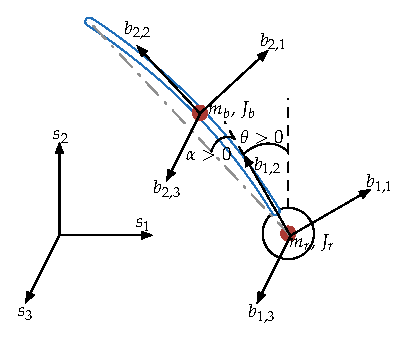
\includegraphics[height=0.352\linewidth,keepaspectratio]{eps/lab_1/rotary_flexible_beam_edit.eps}}
    \caption{(a) Physical rotary flexible beam system~\cite{Q-Flex-Beam}; (b) top view of a 2-DOF model of the physical system with one flexible body and one rigid base, where the flexible body and the rotor base both rotate in the horizontal plane. The reference coordinate axes are shown by $\{s_1,s_2,s_3\}$, the rotor base coordinate axes are shown by $\{b_{1,1},b_{1,2}, b_{1,3}\}$, and the flexible body coordinate axes are shown by $\{b_{2,1},b_{2,2},b_{2,3}\}$. The centres of mass for both bodies are shown in red, and the rotation angle, $\theta$, and deflection angle of the beam's tip, $\alpha$, are shown.}
    \label{fig:lab1_rotary_flexible_beam}
\end{figure}
\subsubsection{The Euler-Lagrange Equation}\label{subsubsection:lab1_EulerLagrange}
\emph{Some mathematical theory:}

The Euler-Lagrange equation is a second-order partial differential equation that will help you find the equations of motion for our physical system. Before presenting the Euler-Lagrange equation, we must first introduce some mathematical objects and notation that have strong physical interpretations.

To describe the configuration of the physical system relative to some reference configuration, we use coordinates (not to be confused with the coordinate axes shown in Figure~\ref{fig:lab1_rotary_flexible_beam} - we're talking about variables $\theta$ and $\alpha$ here) which we call the \emph{generalized coordinates} of the system, and we denote the $i^{th}$ generalized coordinate by $q_i$. We define the kinetic and potential energies of the system by functions of the generalized coordinates and their time derivatives, and denote them by $T$ and $V$, respectively. To summarize the dynamics of our physical system, we use the function $L$ (called the \emph{Lagrangian} of the dynamical system) which is defined by
\[
    L=T-V.
\]
In modelling a physical system, we must also consider external forces applied to the system. We do this by defining a \emph{generalized force} for each generalized coordinate $q_i$ which takes into account the effects of externally applied forces (or torques if $q_i$ is an angle) that are excluded from $V$ (e.g., the force of gravity is a potential force, not a generalized force). We denote the generalized force for $q_i$ by $Q_{q_i}$.
The Euler-Lagrange equation is then given as follows:
\begin{equation}\label{equation:lab1_lagrange_equns}
    \frac{d}{dt} \Bigg(\frac{\partial L}{\partial \dot{q_i}}\Bigg)  - \frac{\partial L}{\partial q_i} = Q_{q_i}.
\end{equation}
To find the equation of motion for a particular coordinate $q_i$, all one must do is find $L$, $V$ and then evaluate~\eqref{equation:lab1_lagrange_equns}.

\emph{Let us jump into modelling our rotary flexible beam}:

We can define the generalized coordinate vector $q(t)^T=[q_1(t) \; q_2(t)]$ using the rotor base angle, $\theta$, and the flexible beam's tip deflection angle, $\alpha$, as follows:
\[
    q(t)^T=[\theta(t) \; \alpha(t)].
\]

Next, we can find the generalized forces (here, they are torques) by simple inspection: since the rotor base is actuated and the flexible beam is not, then one can infer that $Q_\theta = \tau$ and $Q_\alpha = 0$, where $\tau$ is the torque applied by the servo motor. To account for friction, we add viscous friction torques to the generalized forces, giving $Q_\theta = \tau - B_r \dot{\theta}$ and $Q_\alpha = -B_b \dot{\alpha}$, where $B_r$ and $B_b$ are the viscous damping coefficients for the equivalent rotary system and the flexible beam, respectively.

We now find the kinetic and potential energy functions for our rotary flexible beam. To do this, one could consult the model in Figure~\ref{fig:lab1_rotary_flexible_beam}, calculate the moments of inertia of the flexible beam as well as derive the (radial) velocities of the components of the system at their centres of masses using kinematics. The way we are choosing to model the flexible beam is as a \emph{rigid rod connected to a torsional spring}, which flexes by angle $\alpha$; this spring energy can be accounted for in the potential energy term, $V$. Finding $T$ and $V$ isn't related to the scope of this course, so they are given to you:
\begin{equation*}
    \begin{cases}
        T = \frac{1}{2}J_r \dot{\theta}^2 + \frac{1}{2} J_b \left(\dot{\theta}+\dot{\alpha}\right)^2 \\
        V = \frac{1}{2} K_b \alpha^2
    \end{cases}
\end{equation*}
where $K_b$ is the spring torsion coefficient of the flexible beam, $J_r$ is the equivalent moment of inertia of the rotary system, and $J_b$ is the moment of inertia of the flexible beam about its end. One may be able to deduce $T$ and $V$ by thinking about the model shown in Figure~\ref{fig:lab1_rotary_flexible_beam_breakdown}.
\begin{figure}[htb!]
    \centering
    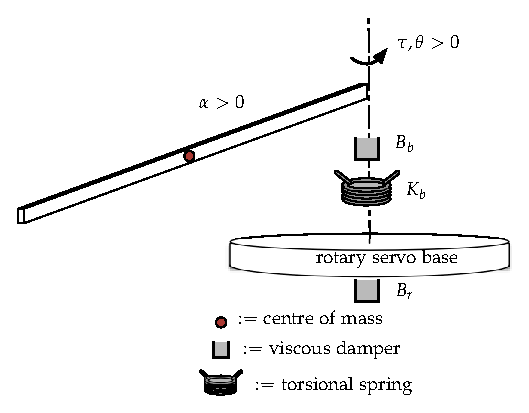
\includegraphics[width=.6\linewidth]{eps/lab_1/rotary_flexible_beam_breakdown_edit.eps}
    \caption{The 2-DOF model used to describe the motion of the rotary flexible beam.}
    \label{fig:lab1_rotary_flexible_beam_breakdown}
\end{figure}
The final steps are left for you to complete $\dots$
\subsubsection{Prelab Questions:}\label{subsubsection:lab1a_prelab}
\begin{enumerate}
    \item What is the equation of motion for generalized coordinate $q_\theta$?\\
          \drew{Answer: it is
              \[
                  \left(J_r + J_b\right)\ddot{\theta} + J_b \ddot{\alpha} = \tau - B_r \dot{\theta}.
              \]
              This is obtained via the Euler-Lagrange equation. One calculates:
              \[
                  \begin{cases}
                      \pder{L}{\theta}=0                                                                                             \\
                      \pder{L}{\dot{\theta}}=J_r\dot{\theta}+J_b\left(\dot{\theta}+\dot{\alpha}\right)                               \\
                      \frac{d}{dt} \left(\pder{L}{\dot{\theta}}\right)= J_r\ddot{\theta}+J_b\left(\ddot{\theta}+\ddot{\alpha}\right) \\
                  \end{cases}
              \]}
    \item What is the equation of motion for generalized coordinate $q_\alpha$?\\
          \drew{Answer: it is
              \[
                  J_b \left(\ddot{\theta} + \ddot{\alpha}\right) + K_b \alpha = -B_b \dot{\alpha}.
              \]
              This is obtained via the Euler-Lagrange equation. One calculates:
              \[
                  \begin{cases}
                      \pder{L}{\alpha}=K_b\alpha                                                                    \\
                      \pder{L}{\dot{\theta}}=J_b\left(\dot{\theta}+\dot{\alpha}\right)                              \\
                      \frac{d}{dt} \left(\pder{L}{\dot{\theta}}\right)= J_b\left(\ddot{\theta}+\ddot{\alpha}\right) \\
                  \end{cases}
              \]}
    \item What is the state-space representation for this system? That is, find $A$ and $B$ and write the EOMs in state-space form.\\
          \textbf{Hint:} Let your state be
          \[
              x(t) =
              \left[\begin{array}{c}
                      \theta(t)       \\
                      \alpha(t)       \\
                      \dot{\theta}(t) \\
                      \dot{\alpha}(t)
                  \end{array}\right].
          \]
          Isolate $\ddot{\theta}$ by subtracting your EOM for $\theta$ by your EOM for $\alpha$. You can let $B_b = 0$ as the viscous damping of the beam is negligible.\\

          \textbf{Important Note:} For your (and your team's) benefit, you may want to complete questions Q7 and Q8 before the lab period, as these questions can be answered more easily by using Mathematica. The ILC controls lab computers do not have Mathematica installed at this time. \\
          \drew{Answer: the state-space representation is
              \[
                  \left[\begin{array}{c}
                          \dot{\theta}(t)  \\
                          \dot{\alpha}(t)  \\
                          \ddot{\theta}(t) \\
                          \ddot{\alpha}(t)
                      \end{array}\right] =
                  \left[\begin{array}{c c c c}
                          0 & 0                                          & 1                & 0 \\
                          0 & 0                                          & 0                & 1 \\
                          0 & \frac{K_b}{J_r}                            & -\frac{B_r}{J_r} & 0 \\
                          0 & -\frac{K_b\left(J_b + J_r\right)}{J_b J_r} & \frac{B_r}{J_r}  & 0
                      \end{array}\right]
                  \left[\begin{array}{c}
                          \theta(t)       \\
                          \alpha(t)       \\
                          \dot{\theta}(t) \\
                          \dot{\alpha}(t)
                      \end{array}\right] \\ +
                  \left[\begin{array}{c}
                          0             \\
                          0             \\
                          \frac{1}{J_r} \\
                          -\frac{1}{J_r}
                      \end{array}\right] \tau
              \]}
\end{enumerate}
\subsection{Working with Simulink \& the Physical System}\label{subsection:lab1_simulink}
Now that you have a state-space representation for the physical system, you can start constructing a Simulink model that will interact with the Quanser SRV02 servo motor in preparation for model validation. Please \textbf{save all of your MATLAB and Simulink files} as you may need to consult them in future labs.
\subsubsection{Setting up the Rotary Flexible Beam}\label{sub subsection:lab1_setup}
First, you must assemble and wire the physical system correctly. Examine the close-up assembly shown in Figure~\ref{fig:lab1_assembly} and replicate this at your workstation. Note that the high-gear configuration is used here: a large gear is connected to a small pinion and a slip gear, rather than using the smaller gear. You will need to build a two-tiered gear train as shown in Figure~\ref{fig:lab1_assembly} to make the large gear fit correctly. Use the wiring diagram shown in Figure~\ref{fig:lab1_wiring} to connect the rotary pendulum to a power source and the data acquisition board.
\begin{figure}[htb!]
    \centering
    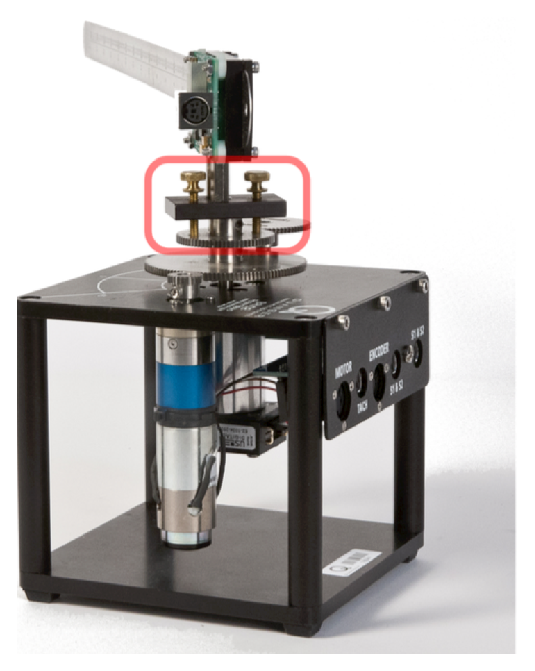
\includegraphics[width=.3\linewidth]{eps/lab_1/assembly.eps}
    \caption{A close-up of the assembly of the rotary flexible beam module and the Quanser SRV02 plant~\cite{Q-Flex-Beam}. The high-gear gear train is indicated by a red box.}
    \label{fig:lab1_assembly}
\end{figure}
\begin{figure}[htb!]
    \centering
    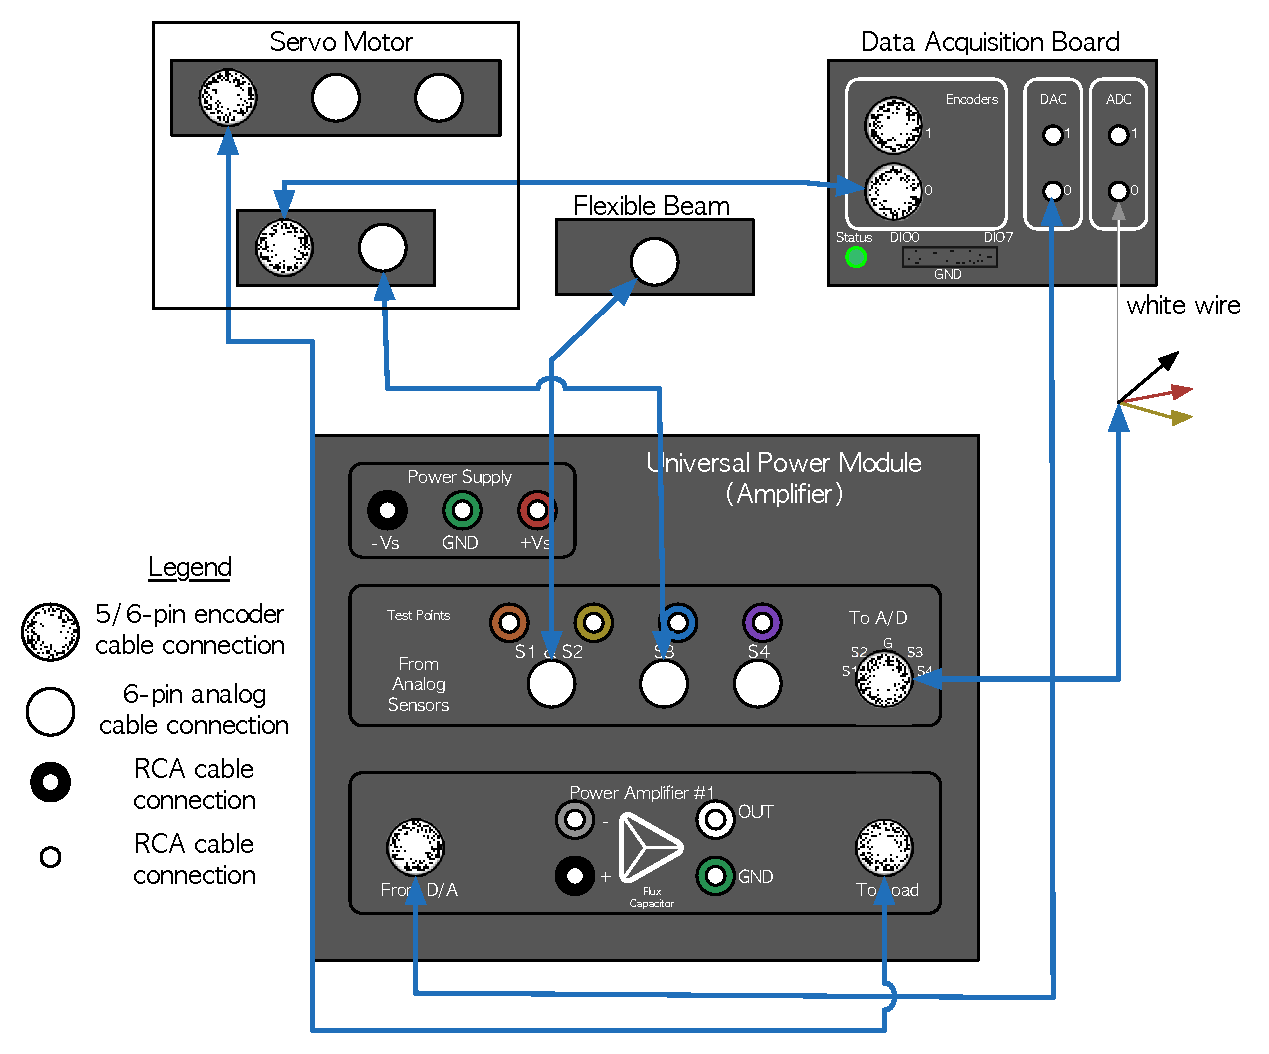
\includegraphics[width=.8\linewidth]{eps/lab_1/wiring.eps}
    \caption{A wiring diagram for the Quanser SRV02 and rotary flexible beam module.}
    \label{fig:lab1_wiring}
\end{figure}
\newpage
\subsubsection{First Simulink Model}\label{lab1_first_model}
You will begin using Simulink by constructing a model including the basic elements required to record the deflection angle of the flexible beam's tip. Here is a step-by-step guide to accomplish this:
\begin{enumerate}
    \item Open MATLAB (\textbf{not the 32-bit version}), type and execute the command ``simulink" in the Command Window. The Simulink Library Browser should appear. Create a new model.
    \item Navigate through the Simulink Library Browser and locate the HIL Initialize block (it is located in QUARC Targets | Data Acquisition | Generic | Configuration). Add this block to your new model, and save the model.
    \item Repeat the same steps to add the HIL Read Analog block (it is located in QUARC Targets | Data Acquisition | Generic | Immediate I/O).
    \item Now, add a Gain block (located in Simulink | Commonly Used Blocks), a R2D block (located in Simulink Extras | Transformations), a To Workspace block (located in Simulink | Sinks), and a Scope block (located in Simulink | Sinks). From the timebase dropdown menu (next to the time box which is used to input a runtime, and is initially set to \emph{inf}), make sure that External is selected. Also, change \emph{inf} to 9.9.
    \item Construct the model as shown in Figure~\ref{fig:lab1_firstmodel}. The HIL Initialize block allows communication between the Quanser SRV02 servo motor, its attached sensors, its added modules and the Simulink model. Double-click on the HIL Initialize block to access its Source Block Parameters. In the Main tab, select ``q2\_usb" as \emph{Board type} from the options list (USB is the interface we use to connect the Quanser Data Acquisition board to our computer). In the Analog Outputs tab, only check the checkboxes 4, 5 and 6 out of the seven (I'm numbering them in increasing order from the top). In the Digital Outputs tab, enter [0:7] in the \emph{Digital output channels} text box. In the last three text boxes for \emph{Initial digital outputs}, \emph{Final digital outputs} and \emph{Digital outputs watchdog expiry}, enter [0].
    \item The HIL Read Analog block is used to record the flexible beam's deflection angle, $\alpha$, via an analog strain gauge sensor located at the end of the beam. Double-click on the HIL Read Analog block to access its Source Block Parameters. Set your \emph{Board name} to HIL-1 to assign this source block to the HIL Initialize block that you previously configured. Next, set your \emph{Channels} to [0], as this is the channel that your strain gauge sensor is connected to.
    \item The Gain block is used to calibrate strain gauge. Double-click on the Gain block to access its Function Block Parameters. Under the Main tab, set your \emph{Gain} to $\frac{1}{16.5}$. Under the Signal Attributes tab, check the \emph{Saturate on integer flow} check box. Under the Parameter Attributes tab, select ``Inherit: Same as Input" in the list of options for \emph{Parameter data type}.
    \item The Scope block is used to plot the readings of $\alpha$ with respect to time. Rename the block to ``alpha (degrees)".
    \item The To Workspace block is used to send the flexible beam's tip deflection angle to the workspace so that it can be plotted/manipulated in MATLAB. Double-click on the To Workspace block and under the \emph{Save Format} options list, choose Structure With Time. Rename the block appropriately.
    \item \textbf{Before running any Simulink file containing Quanser blocks, you must type in \emph{mex -setup} into the MATLAB command window. You will be prompted to answer three questions in sequence; the answers are: \emph{y}, \emph{1}, and \emph{y}.}
\end{enumerate}
\begin{figure}[htb!]
    \centering
    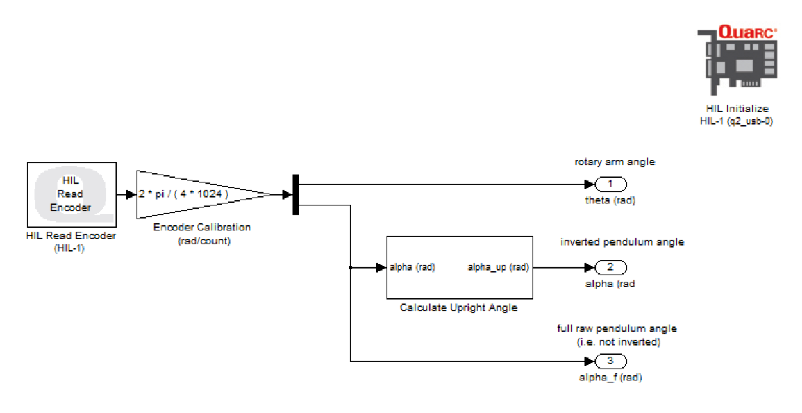
\includegraphics[width=.7\linewidth]{eps/lab_1/first_model.eps}
    \caption{The first Simulink model required for this lab.}
    \label{fig:lab1_firstmodel}
\end{figure}

\textbf{Note:} The \emph{power amplifier must be turned on} before you can experiment with the physical system. The power switch is located at the back of the amplifier (good luck finding it). Make sure to turn off the power amplifier at your station before you leave the lab.

You won't have to construct all of the Simulink models for each lab, but you will have to add some blocks to modify existing and provided models to make them do exactly what you want. So it will benefit you to have an understanding of how a Simulink model and a physical system interact.
\subsubsection{Finding the spring torsion of the Flexible Beam Experimentally}\label{subsubsection:lab1_spring_stiffness}
\emph{Let us review some vibrations theory:}

In the 2-DOF model, we use a spring torsion coefficient, $K_b$, to characterize the potential energy of the system due to the beam's deflections. In order to find the value of $K_b$, you can perturb the physical flexible beam while holding the rotor base stationary and study its deflection response. Consider a system response as shown in Figure~\ref{fig:lab1_perturbation_response}; you can find the average period of the deflection oscillations, $T_\text{osc}$, by using
\begin{equation}\label{lab1_oscillation_period}
    T_\text{osc} = \frac{t_{n+1}-t_1}{n},
\end{equation}
where $n$ is the n\textsuperscript{th} oscillation and $t_i$ is the occurrence time of the i\textsuperscript{th} oscillation, for $i \in \{1, \dots,n+1\}$. To find $T_\text{osc}$ using~\eqref{lab1_oscillation_period}, you should always measure oscillation occurrence times from the same datum. Using the average period, you are able to find the damped natural frequency, $\omega_d$, of the system with
\[
    \omega_d = \frac{2\pi}{T_\text{osc}},
\]
and the natural frequency, $\omega_n$ is related to $\omega_d$ by
\begin{equation}\label{lab1_natural_frequency}
    \omega_n = \frac{w_d}{\sqrt{1-\zeta^2}},
\end{equation}
where $\zeta$ is the damping ratio of the system. For second-order systems, one can find the damping ratio using the logarithmic decrement equation, but for our flexible beam system $\zeta<<1$ (underdamped case) and thus $\omega_d \approx \omega_n$ by~\eqref{lab1_natural_frequency}. Finally, you can calculate the spring torsion coefficient of the flexible beam by using the relationship
\[
    K_b = J_b \omega_{n}^2,
\]
which is valid for second-order systems. Recall that the moment of inertia of a thin rod about its end is given by $J_b = \frac{1}{3} m_b L_{b}^2$.\\
\emph{Back to your lab:}

Using the Simulink file that you created in \hyperref[subsection:lab1_simulink]{Section~\ref{subsection:lab1_simulink}}, you can now find $K_b$ given the following constants:
\[
    \begin{cases}
        m_b = 0.065 \; kg \\
        L_b = 0.419 \; m
    \end{cases}
\]
You will have to build your Simulink model. To do this, access the QUARC drop-down menu, and select \emph{Build} (or simply type \emph{Ctrl + B}).
\begin{figure}[htb!]
    \centering
    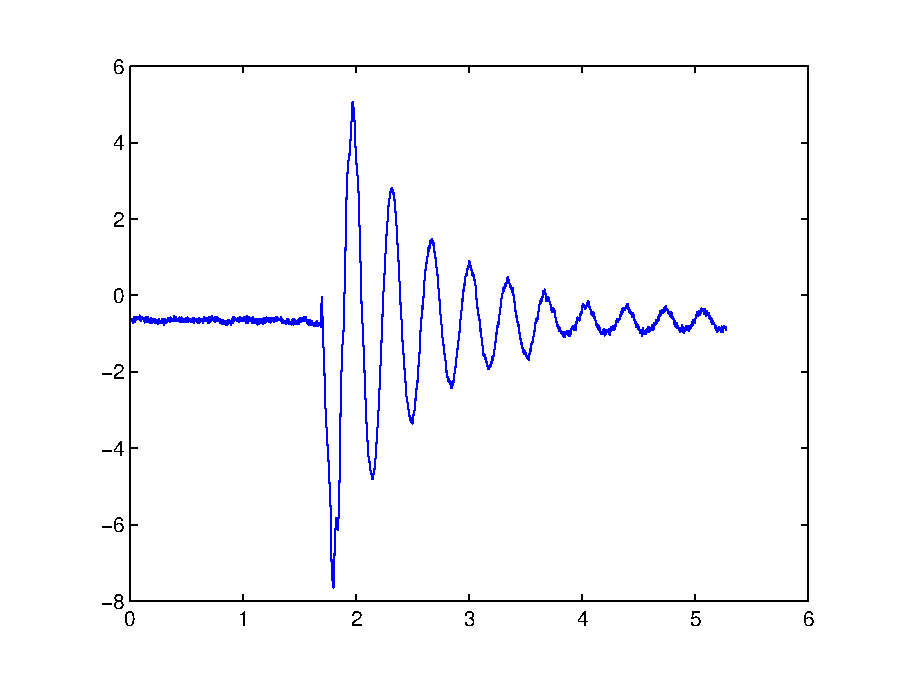
\includegraphics[width=.5\linewidth]{eps/lab_1/perturb.eps}
    \caption{An example of a response of the flexible beam's deflection angle $\alpha$ to a perturbation while rotor base is held stationary.}
    \label{fig:lab1_perturbation_response}
\end{figure}
\begin{enumerate}[Questions]
    \item[Q1:] What is the natural frequency of the physical flexible beam? Include a plot of the flexible beam response to your perturbation.\\
          \drew{Answer: You should get close to
              \[
                  T_\text{osc} = \frac{3.8-2.1}{5} = 0.34 s
              \]
              \[
                  \omega_n = \frac{2\pi}{0.34} = 18.5 \frac{rad}{s}
              \]
              and the plot should look very similar to Figure~\ref{fig:lab1_perturbation_response}.
          }
    \item[Q2:] What is the spring torsion coefficient of the flexible beam, $K_b$?\\
          \drew{Answer: You should get close to
              \[
                  K_b = \frac{m_b L_{b}^2}{3} \omega_{n}^2 = 1.3 \frac{N \cdot m}{rad}
              \]
          }
\end{enumerate}

\subsubsection{Model Validation}\label{subsubsection:lab1_modelvalidation}
You are now in the position to test how accurate your 2-DOF state-space model of the physical system is. To do this, you will compare the response of your state-space model and that of the physical system to an input.

You will start off by modifying an existing Simulink model by adding your state-space model in parallel to the existing physical system model. Open the file \\ \textbf{model\_validation.mdl} and examine the existing model, shown in Figure~\ref{fig:lab1_model_validation_student}. This Simulink model can instruct the physical system's servo motor to track a step function; while tracking the input, the servo motor encoder and strain gauge readings will measure and output the rotor angle and beam tip's deflection angle with respect to time.
\begin{figure}[htb!]
    \centering
    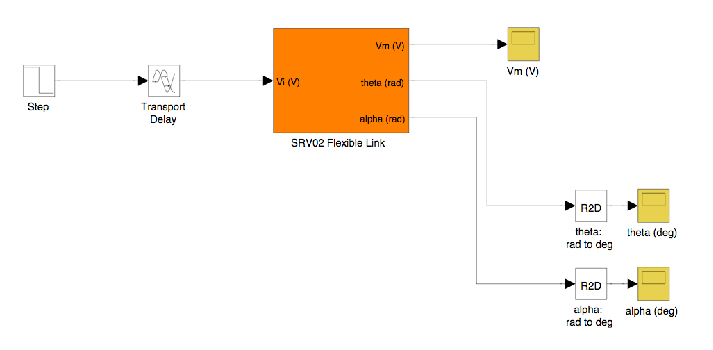
\includegraphics[width=.7\linewidth]{eps/lab_1/model_validation_student.eps}
    \caption{A screenshot of the exisiting Simulink model, \textbf{model\_validation.mdl}.}
    \label{fig:lab1_model_validation_student}
\end{figure}

You wish to compare the responses of both the physical system and state-space model to a step input. To do this, you will need to add a State-Space block (located in Simulink | Continuous). You will need to feed your state-space block with the same step input as is being fed to your physical system. You will eventually enter in your state-space matrices $A$, $B$, $C$ and $D$ in the MATLAB workspace, so in order for your State-Space block to recognize these in Simulink, set its Function Block Parameters for $A$, $B$, $C$ and $D$ as themselves (i.e., A: as ``A"). Furthermore, you'll need to output the states $\theta$ and $\alpha$ (i.e., states 1 and 2 of the four states) from your state-space block to the existing scope blocks for $\theta$ and $\alpha$. To access only states 1 and 2 from your State-Space block, you can make use of the Demux block (located in Simulink | Commonly Used Blocks), which splits vector signals into scalars or smaller vectors. To join alike states from your state-space model and your physical model, you can use the Mux block, which works like the inverse of the Demux block.\\
\drew{The correct Simulink model looks something like:
    \begin{figure}[htb!]
        \centering
        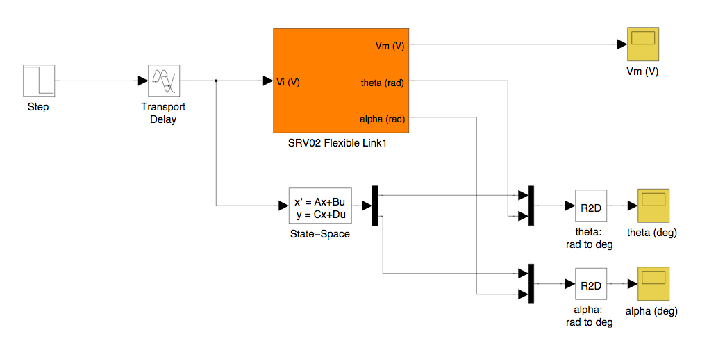
\includegraphics[width=.6\linewidth]{eps/lab_1/model_validation.eps}
        \caption{A screenshot of the correctly-modified Simulink model}
        \label{fig:lab1_model_validation}
    \end{figure}
}

Now, you must evaluate the symbolic matrices you found for $A$ and $B$, which involves finding the equivalent moment of inertia for the rotary flexible beam system. Finding $J_r$ is quite a challenging problem: it involves finding the external gears inertias, the motor equivalent inertia, the motor shaft inertia, the load inertia (in this case, the load is the flexible beam module), and relating these parameters via gear ratios while considering gearbox efficiency. Furthermore, finding the equivalent viscous damping for the system is usually done experimentally. For these reasons, the values for $J_r$ and $B_r$ are given here:
\[
    \begin{cases}
        J_r = 0.0020841 \; kg \cdot m^2   \\
        J_b = 0.0038038 \; kg \cdot m^2   \\
        B_r = 0.015 \; \frac{N\cdot s}{m} \\
        B_b = 0 \; \frac{N\cdot s}{m} \; \text{(negligible beam damping)}
    \end{cases}
\]
Recall that the moment of inertia of the flexible beam about its end is given by $J_b = \frac{1}{3} m_b L_{b}^2$ (by assuming that the flexible beam can be modelled as an infinitely thin but rigid rod), so you can calculate this explicitly to evaluate your state-space matrices. Another consideration is that the servo motor actuator is controlled by voltage and not by torque (the resulting motor torque is a function of the voltage applied by the servo motor). To transform the state-space model from your prelab in terms of voltage, one must do the following in sequence:
\begin{enumerate}
    {\indentitem \item[Step 1:] let matrix entry $A(3,3) = A(3,3) - \eta_g \eta_m \cdot \frac{K_{g}^2 k_t k_m}{R_m} B(3)$, where $K_g=70$ is the total gear ratio for your setup, $k_t=0.0077$ is the servo motor torque constant, $k_m = 0.0077$ is the motor back-EMF constant, $\eta_g = 0.90$ is the gear efficiency, $\eta_m = 0.69$ is the motor efficiency, and $R_m=2.6$ is the motor armature resistance;} \\
          {\indentitem \item[Step 2:] let matrix entry $A(4,3) = A(4,3) - \eta_g \eta_m \cdot \frac{K_{g}^2 k_t k_m}{R_m} B(4)$;} \\
          {\indentitem \item[Step 3:] only now should you modify $B$ to $B = \eta_g \eta_m \cdot \frac{K_g k_t}{R_m} B$.}
\end{enumerate}
\textbf{We've prepared a MATLAB script for you to speed up the process}: open \\
\textbf{lab1\_statespace\_student}, input your symbolic matrices that you computed in your prelab, and run the script to evaluate your state-space matrices $A$ and $B$.
\begin{enumerate}[Question]
    \item[Q3:] What are the numerically-evaluated matrices $A$ and $B$ for the state-space model?\\
          \drew{Answer: You should get
              \[
                  A =
                  \left[\begin{array}{c c c c}
                          0 & 0       & 1      & 0 \\
                          0 & 0       & 0      & 1 \\
                          0 & 623.77  & -40.49 & 0 \\
                          0 & -965.53 & 40.49  & 0
                      \end{array}\right]
              \]
              and
              \[
                  B =
                  \left[\begin{array}{c}
                          0      \\
                          0      \\
                          61.775 \\
                          -61.775
                      \end{array}\right].
              \]
          }
    \item[Q4:] Given that the physical system's sensors are limited to reading the rotor angle and the deflection angle, what should the numerical matrices $C$ and $D$ for the state-space model be? Pay attention to matrix dimensions here.\\
          \drew{Answer: You should get
              \[
                  C =
                  \left[\begin{array}{c c c c}
                          1 & 0 & 0 & 0 \\
                          0 & 1 & 0 & 0
                      \end{array}\right]
              \]
              and
              \[
                  D =
                  \left[\begin{array}{c}
                          0 \\
                          0
                      \end{array}\right],
              \]
              which can be discerned from the state-space equation $y = Cx + Du$.
          }
\end{enumerate}

With your modified Simulink model and evaluated matrices, you can now build your Simulink model and see whether your state-space model accurately describes the physical system. Make sure that you have entered $A$, $B$, $C$, and $D$ into the MATLAB command window and set the run time in the top toolbar of your Simulink model to 9.9. Now, select the \emph{Quarc} drop-down menu from the main toolbar and click Build. Make sure that both signals (i.e., the physical system's and the state-space model's) are converted to degrees via the \emph{R2D} Simulink block. When you are ready, click Run, which can be found in the same drop-down menu. Plot the $\theta$ and $\alpha$ arrays with respect to time, and include these plots in your lab report.
\begin{enumerate}[Question]
    \item[Q5:] How well does your model represent the physical system? Give one good reason why the model doesn't have an identical response to that of the physical system.\\
          \drew{Answer: The model represents the system quite well. The flexible beam model's response (i.e., $\alpha$-time plot) matches the physical system's response very well for the first few oscillations, but doesn't capture the lower amplitude oscillations and the higher frequency oscillations. This is due to the fact that the flexible beam is modelled as a torsional spring \& rigid beam and not as a higher-order nonlinear beam. The rotor base model's response (i.e., $\theta$-time plot) has a steady-state error which is probably due to Coulomb friction or not having an accurate $B_r$. The plots should look something like this:
              \begin{figure}[htb!]
                  \centering
                  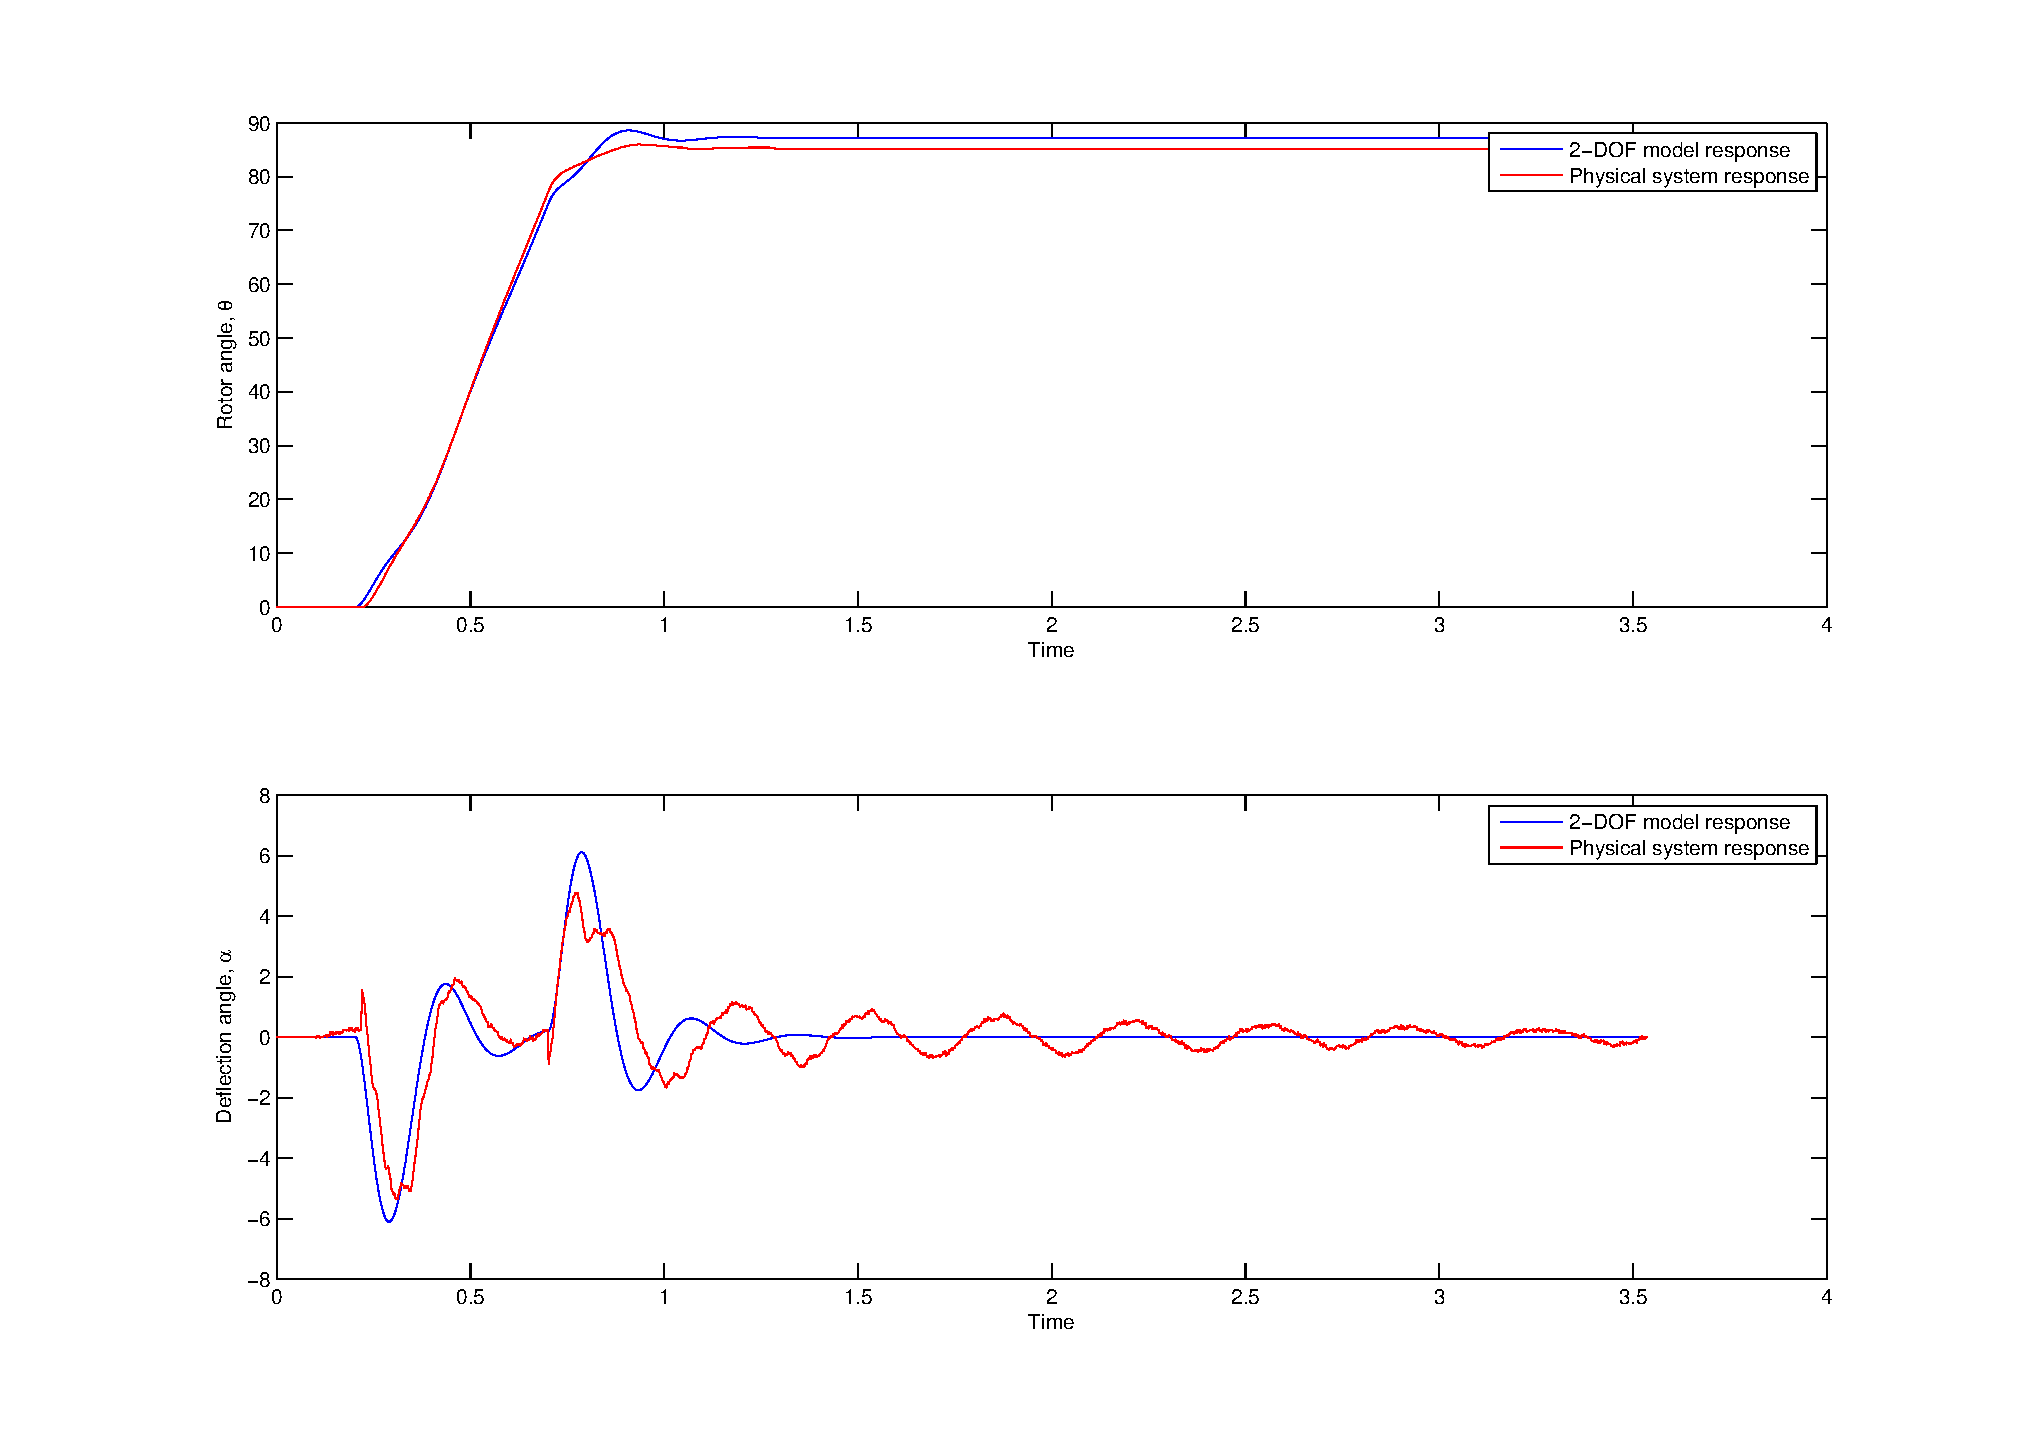
\includegraphics[width=.8\linewidth]{eps/lab_1/model_validation_plots.eps}
                  \caption{The correct plots of $\theta$ and $\alpha$ w.r.t. time for the model \& physical system response to a step input.}
                  \label{fig:lab1_model_validation__step2to0}
              \end{figure}
          }
\end{enumerate}
Recall that we used a \emph{linear spring} to model the flexible beam in our system, and by doing so we were able to use $V=\frac{1}{2}K_b \alpha^2$ to characterize the system's potential energy. This is like making a linear approximation as the flexible beam is likely to deflect nonlinearly and as a function of the length along the beam. To test where your approximation and hence your state-space model is valid, you will use larger step inputs and compare the responses of your model and of the physical system.
\begin{enumerate}[Question]
    \item[Q6:] How accurate is your state-space model when the input step response is increased from 2 to 3 as an initial value? What about increasing the input step response's initial value from 2 to 4? Give a plot of the responses of $\alpha$ of your model and the physical system.\\
          \drew{The higher frequency vibrations of the physical system are more prevalent and are not captured by the 2-DOF model. Hence the model is less accurate with a larger input. The plots should look like:
              \begin{figure}[htb!]
                  \centering
                  \subfigure[]{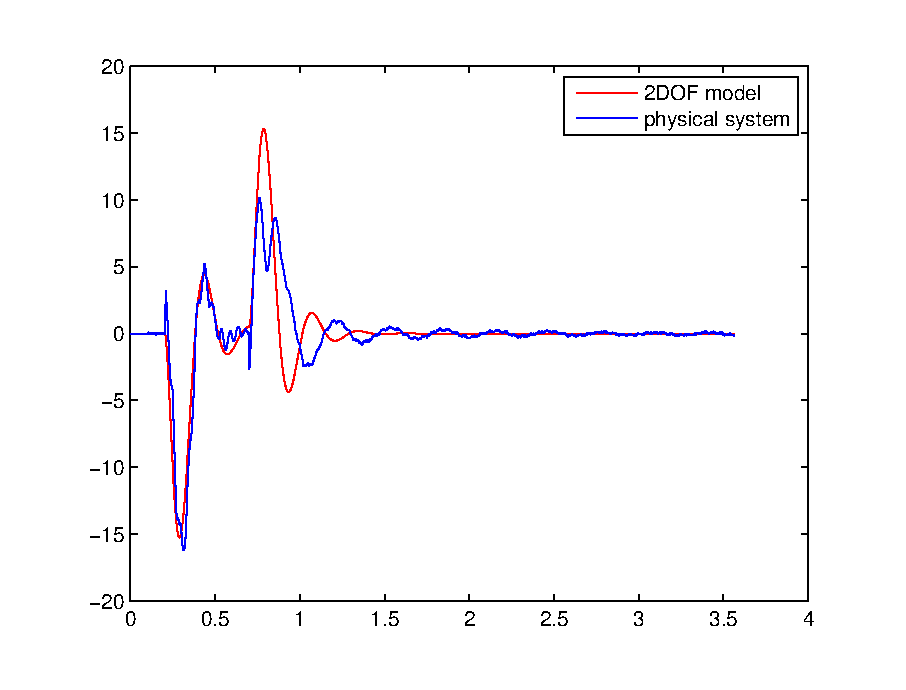
\includegraphics[width=.4\linewidth]{eps/lab_1/step_5to0_2DOF_physical.eps}} \quad
                  \subfigure[]{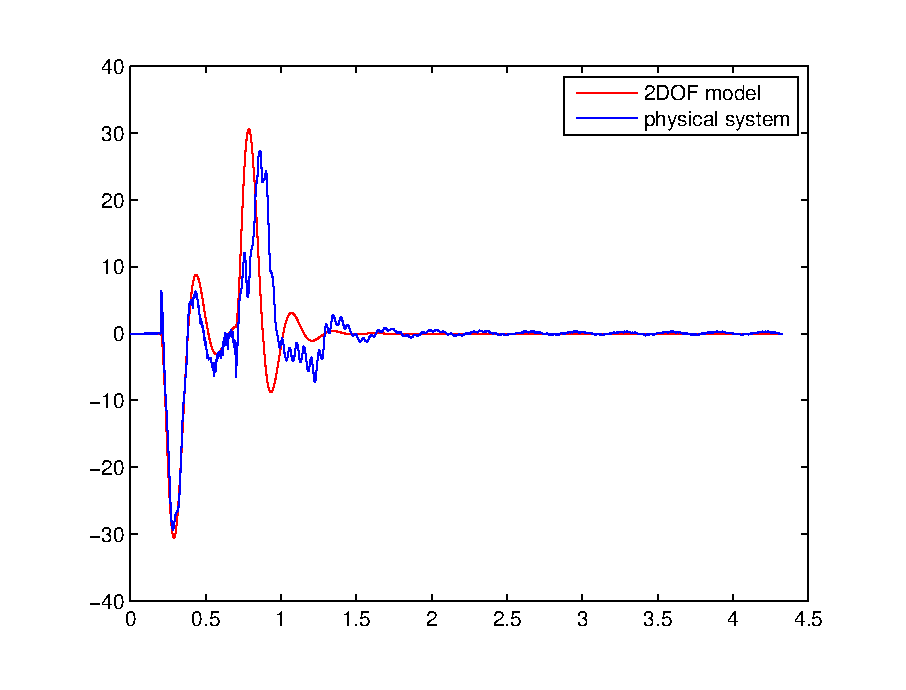
\includegraphics[width=.4\linewidth]{eps/lab_1/step_10to0_2DOF_physical.eps}}
                  \caption{The correct plot of $\theta$ and $\alpha$ w.r.t. time for the model \& physical system response to a step input with initial value of a) 5 and b) 10.}
                  \label{fig:lab1_model_validation_step5to0}
              \end{figure}
          }
\end{enumerate}
\newpage
\subsection{Higher-Order Model for the Flexible Beam}\label{subsection:lab1_higher_order}
\begin{figure}[htb!]
    \centering
    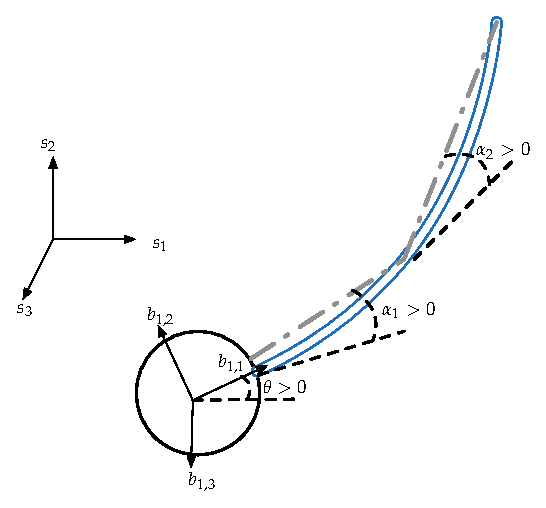
\includegraphics[width=.5\linewidth]{eps/lab_1/rotary_flexible_beam_3DOF_edit}
    \caption{Top view of a 3-DOF model of the rotary flexible beam. The reference coordinate axes are shown by $\{s_1,s_2,s_3\}$, the rotor base coordinate axes are shown by $\{b_{1,1},b_{1,2}, b_{1,3}\}$, and the two flexible beam body coordinate axes are left out for clarity.  The rotation angle, $\theta$, and the deflection angles, $\alpha_1$ and $\alpha_2$, are shown.}
    \label{fig:lab1_rotary_flexible_beam_3DOF}
\end{figure}
As was discussed earlier, a realistic model for a flexible beam involves an infinite-dimensional system. As modelling an infinite-dimensional system is an intractable problem from an engineering standpoint, one can approximate this system by breaking it up into a set of finite elements with solvable problems. You will do this with the rotary flexible beam system by introducing another deflection angle, making the system a 3-DOF system and changing the generalized coordinate vector to
\[
    q(t) = \left[\begin{array}{c}
            \theta(t)   \\
            \alpha_1(t) \\
            \alpha_2(t)
        \end{array}\right],
\]
where $\alpha_1$ measures the deflection angle from the starting point to the midpoint of the beam, and $\alpha_2$ measures the deflection angle from the midpoint to the end of the beam. Refer to Figure~\ref{fig:lab1_rotary_flexible_beam_3DOF} for a schematic of these deflection angles. As was done for the 2-DOF system, we will use linear springs and account for viscous damping for each half-element of the beam. The kinetic and potential energies for the 3-DOF system are given:
\[
    \begin{cases}
        T = \frac{1}{2} J_r \dot{\theta}^2 + \frac{1}{2} J_{b_1} \left(\dot{\theta} + \dot{\alpha}_1\right)^2 + \frac{1}{2} J_{b_2} \left(\dot{\theta} + \dot{\alpha}_1 + \dot{\alpha}_2\right)^2 \\
        V = \frac{1}{2} K_{b_1}\alpha_{1}^2 + \frac{1}{2} K_{b_2} \alpha_{2}^2
    \end{cases}
\]
where $J_{b_1}$ and $J_{b_2}$ are the moment of inertias of the first half-element and the second half-element about their ends, and $K_{b_1}$ and $K_{b_2}$ are the spring torsion coefficients of the first and second half-elements, respectively. In this higher-order system, the generalized force (torques here) for coordinate $\theta$ remains the same, and those for coordinates $\alpha_1$ and $\alpha_2$ can be reasoned out. They are given:
\[
    \begin{cases}
        Q_\theta = \tau - B_r \dot{\theta}     \\
        Q_{\alpha_1} = -B_{b_1} \dot{\alpha_1} \\
        Q_{\alpha_2} = -B_{b_2} \left(\dot{\alpha_1}+\dot{\alpha_2}\right).
    \end{cases}
\]
\begin{figure}[htb!]
    \centering
    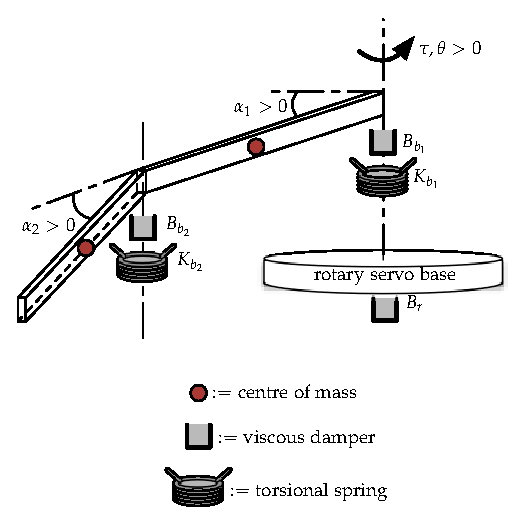
\includegraphics[width=.5\linewidth]{eps/lab_1/rotary_flexible_beam_3DOF_breakdown_edit.eps}
    \caption{The 3-DOF model used to describe the motion of the rotary flexible beam.}
    \label{fig:lab1_rotary_flexible_beam_3DOF_breakdown}
\end{figure}
One can deduce that $J_{b_1} = J_{b_2} = \frac{1}{4} J_b$, as these are symmetric half-elements of the flexible beam. Applying the angular form of Hooke's Law, $T=K_b\alpha$, where $T$ is the torque exerted by the spring, the spring torsion coefficients can be related: $K_{b_1} = K_{b_2}$, where $K_{b_1} = 2 K_b$, as we are using linear springs. One can also use a result from the study of vibrations for underdamped systems to relate the viscous damping coefficients of both half-elements:
\[
    \zeta = \frac{B}{2\sqrt{J_b K}}
\]
where  $\zeta$ is the damping ratio of the flexible beam and $J_b$ is the moment of inertia of the flexible beam. The viscous damping coefficients are then related as follows: $B_{b_1} = B_{b_2}$, where $B_{b_1} = \sqrt{2} B_b$. You may want to consult Figure~\ref{fig:lab1_rotary_flexible_beam_3DOF_breakdown} to intuitively think about this 3-DOF model.
You now have enough information to find the EOMs for this system \dots.
\begin{enumerate}[Question]
    \item[Q7:] What are the three equations of motion for the higher-order system?\\
          \textbf{Hint:} Isolate $\ddot{\theta}$ by subtracting your EOM for $\theta$ by your EOM for $\alpha_1$ (similar to what you did in the prelab). You can let $B_{b_1} = B_{b_2} = \sqrt{2}B_b = 0$ as the viscous damping of the beam is negligible. \textbf{You may want to use Mathematica} to speed up the process of isolating these EOMs for $\ddot{\theta}$, $\ddot{\alpha_1}$ and $\ddot{\alpha_2}$.\\
          \drew{Answer: the EOMs are
              \[
                  \begin{cases}
                      \ddot{\theta} = \frac{K_{b_1}}{J_r} \alpha_1 + \frac{B_{b_1}}{J_r} \dot{\alpha_1} + -\frac{B_r}{J_r} \dot{\theta} + \frac{\tau}{J_r}                                                                                                                             \\
                      \\
                      \ddot{\alpha}_1 = \left(\frac{-K_{b_1}}{J_r}-\frac{2 K_{b_1}}{J_b}\right)\alpha_1 + \frac{2 K_{b_2}}{J_b}\alpha_2 + \left(\frac{-B_{b_1}}{J_r} - \frac{2 B_{b_1} - 2 B_{b_2}}{J_b}\right)\dot{\alpha}_1 + \frac{2 B_{b_2}}{J_b}\dot{\alpha}_2 - \frac{\tau}{J_r} \\
                      \\
                      \ddot{\alpha}_2 = \frac{2 K_{b_1}}{J_b}\alpha_1 - \frac{4 K_{b_2}}{J_b}\alpha_2 + \frac{2 B_{b_1} - 4 B_{b_2}}{J_b}\dot{\alpha}_1 - \frac{4 B_{b_2}}{J_b}\dot{\alpha}_2
                  \end{cases}
              \]
              To find these, one can use the Euler-Lagrange equations. We first compute the following:
              \[
                  \begin{cases}
                      \pder{L}{\theta} = 0                                                                                                                                                \\
                      \pder{L}{\alpha_1}=-K_{b_1}\alpha_1                                                                                                                                 \\
                      \pder{L}{\alpha_2}=-K_{b_2} \alpha_2                                                                                                                                \\
                      \pder{L}{\dot{\theta}}= J_r\dot{\theta}+J_{b_1}(\dot{\theta}+\dot{\alpha}_1) + J_{b_2}(\dot{\theta}+\dot{\alpha}_1+\dot{\alpha}_2)                                  \\
                      \pder{L}{\dot{\alpha}_1} =J _{b_1}(\dot{\theta}+\dot{\alpha}_1) + J_{b_2}(\dot{\theta}+\dot{\alpha}_1+\dot{\alpha}_2)                                               \\
                      \pder{L}{\dot{\alpha}_2} =J_{b_2}(\dot{\theta}+\dot{\alpha}_1+\dot{\alpha}_2)                                                                                       \\
                      \frac{d}{dt} \left(\pder{L}{\dot{\theta}}\right) = J_r\ddot{\theta}+J_{b_1}(\ddot{\theta}+\ddot{\alpha}_1) + J_{b_2}(\ddot{\theta}+\ddot{\alpha}_1+\ddot{\alpha}_2) \\
                      \frac{d}{dt} \left(\pder{L}{\dot{\alpha}_1}\right) = J_{b_1}(\ddot{\theta}+\ddot{\alpha}_1) + J_{b_2}(\ddot{\theta}+\ddot{\alpha}_1+\ddot{\alpha}_2)                \\
                      \frac{d}{dt} \left(\pder{L}{\dot{\alpha}_2}\right) = J_{b_2}(\ddot{\theta}+\ddot{\alpha}_1+\ddot{\alpha}_2)                                                         \\
                  \end{cases}
              \]
              This yields the following EOMs:
              \[
                  \begin{cases}
                      J_r \ddot{\theta} + J_{b_1} (\ddot{\theta}+\ddot{\alpha}) + J_{b_2}(\ddot{\theta}+\ddot{\alpha}_1+\ddot{\alpha}_2) = \tau-B_r\dot{\theta}   \\
                      J_{b_1} (\ddot{\theta}+\ddot{\alpha}) + J_{b_2}(\ddot{\theta}+\ddot{\alpha}_1+\ddot{\alpha}_2) + K_{b_1} \alpha_1 = -B_{b_1} \dot{\alpha}_1 \\
                      J_{b_2}(\ddot{\theta}+\ddot{\alpha}_1+\ddot{\alpha}_2) + K_{b_2} \alpha_2 = -B_{b_1} (\dot{\alpha}_1+\dot{\alpha}_2).
                  \end{cases}
              \]
              To isolate these EOMs in terms of $\ddot{\theta}, \ddot{\alpha}_1, \ddot{\alpha}_2$, subtract the first equation by the second to yield the first isolated EOM:
              \[
                  \ddot{\theta} = \frac{K_{b_1}}{J_r} \alpha_1 + \frac{B_{b_1}}{J_r} \dot{\alpha_1} + -\frac{B_r}{J_r} \dot{\theta} + \frac{\tau}{J_r}.
              \]
              Next, substitute this EOM (isolated for $\ddot{\theta}$) into the third equation, and then substitute the second equation thereafter to get:
              \[\ddot{\alpha}_1 = \left(\frac{-K_{b_1}}{J_r}-\frac{2 K_{b_1}}{J_b}\right)\alpha_1 + \frac{2 K_{b_2}}{J_b}\alpha_2 + \left(\frac{-B_{b_1}}{J_r} - \frac{2 B_{b_1} - 2 B_{b_2}}{J_b}\right)\dot{\alpha}_1 + \frac{2 B_{b_2}}{J_b}\dot{\alpha}_2 - \frac{\tau}{J_r}.\]
              You can now solve for the third EOM (isolating for $\ddot{\alpha}_2$) by substituting. If you followed these steps, you now know how tedious engineering could be$\dots$
          }
    \item[Q8:] What is the state-space representation for this system? Please include $A$, $B$, $C$ and $D$ with symbolic entries.\\
          \drew{Answer: your state vector should be
              \[
                  \left[\begin{array}{c}
                          \theta         \\
                          \alpha_1       \\
                          \alpha_2       \\
                          \dot{\theta}   \\
                          \dot{\alpha}_1 \\
                          \dot{\alpha}_2
                      \end{array}\right]
              \]
              and your resulting symbolic matrices for $A$ and $B$ should be
              \[A=
                  \left[\begin{array}{c c c c c c}
                          0 & 0                                                       & 0                      & 1 & 0                                                                             & 0                      \\
                          0 & 0                                                       & 0                      & 0 & 1                                                                             & 0                      \\
                          0 & 0                                                       & 0                      & 0 & 0                                                                             & 1                      \\
                          0 & \frac{K_{b_1}}{J_r}                                     & 0                      & 0 & \frac{B_{b_1}}{J_r}                                                           & 0                      \\
                          0 & \left(\frac{-K_{b_1}}{J_r}-\frac{2 K_{b_1}}{J_b}\right) & \frac{2 K_{b_2}}{J_b}  & 0 & \left(\frac{-B_{b_1}}{J_r}-\frac{2 B_{b_1}}{J_b}+\frac{2 B_{b_2}}{J_b}\right) & \frac{2 B_{b_2}}{J_b}  \\
                          0 & \frac{2 K_{b_1}}{J_b}                                   & \frac{-4 K_{b_2}}{J_b} & 0 & \frac{2 B_{b_1}- 4 B_{b_2}}{J_b}                                              & \frac{-4 B_{b_2}}{J_b}
                      \end{array}\right],
              \]
              \[B=
                  \left[\begin{array}{c}
                          0              \\
                          0              \\
                          0              \\
                          \frac{1}{J_r}  \\
                          \frac{-1}{J_r} \\
                          0
                      \end{array}\right].
              \]
              As we wish to output all three states, we have that
              \[C =
                  \left[\begin{array}{c c c c c c}
                          1 & 0 & 0 & 0 & 0 & 0 \\
                          0 & 1 & 0 & 0 & 0 & 0 \\
                          0 & 0 & 1 & 0 & 0 & 0 \\
                      \end{array}\right],
              \]
              \[D =
                  \left[\begin{array}{c c c}
                          0 \\
                          0 \\
                          0
                      \end{array}\right].
              \]}
\end{enumerate}

Recall that the state-space matrices must be transformed to account for a voltage input rather than a torque input, as was done for the 2-DOF system. Using the state-space model that you came up with, you can now create a Simulink model to simulate your state-space model's response to a step function, as was done in \hyperref[subsubsection:lab1_modelvalidation]{Section~\ref{subsubsection:lab1_modelvalidation}}. You may build a Simulink model similar to that shown in Figure~\ref{fig:lab1_higher_order_simulink_model}, following the steps and using the same input as in \hyperref[subsubsection:lab1_modelvalidation]{Section~\ref{subsubsection:lab1_modelvalidation}}. You will again have to follow the steps to convert the model from a torque input to a voltage input (except now the matrix indices are slightly different as there are two more states). You will compare the 3-DOF model's responses to all three step inputs that were used in \hyperref[subsubsection:lab1_modelvalidation]{Section~\ref{subsubsection:lab1_modelvalidation}}.

\begin{figure}[htb!]
    \centering
    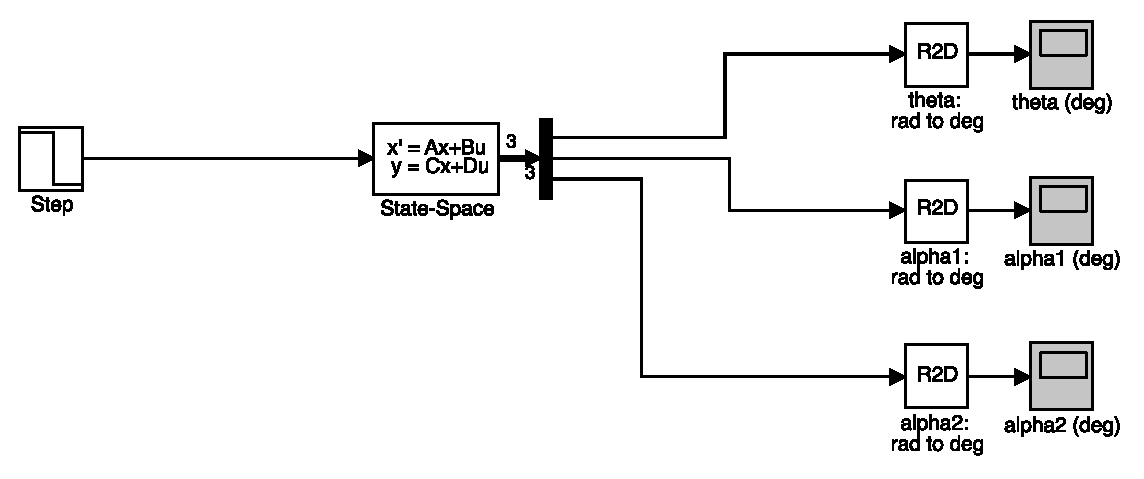
\includegraphics[width=.7\linewidth]{eps/lab_1/higher_order_simulink_model}
    \caption{A candidate Simulink model to simulate and output the response of the 3-DOF system to the step input used for the 2-DOF system.}
    \label{fig:lab1_higher_order_simulink_model}
\end{figure}

\begin{enumerate}[Question]
    \item[Q9:]How will you compare the 3-DOF model's response to the physical system's response as was found in \hyperref[subsubsection:lab1_modelvalidation]{Section~\ref{subsubsection:lab1_modelvalidation}}, using your Simulink data?\\
          \drew{Answer: You should add $\alpha_1$ and $\alpha_2$, and then compare this value's response to that of the physical system's.}
    \item[Q10:] Compare the 2-DOF and 3-DOF model's accuracy by comparing their individual responses to that of the physical system, as was found in \hyperref[subsubsection:lab1_modelvalidation]{Section~\ref{subsubsection:lab1_modelvalidation}}. Do this for all three step inputs, i.e., step inputs starting at 2, 3 and 4. Which model is more accurate for these step inputs? Does modelling a physical system with a higher-order model ensure better accuracy?\\
          \drew{Answer: In some instances, the 3-DOF model is slightly more accurate than the 2-DOF model in describing the motion of the flexible beam \textbf{when $B_{b_1} \not = 0$}. This makes sense physically, because one needs a nonzero damping term on the first-half of the flexible beam to ensure that the second-half of the flexible beam not go unstable. A higher-order model is not always better: one must verify the physical feasibility of a model and make sure that the additional discretization be representative of the physical system.}
          \begin{figure}[htb!]
              \centering
              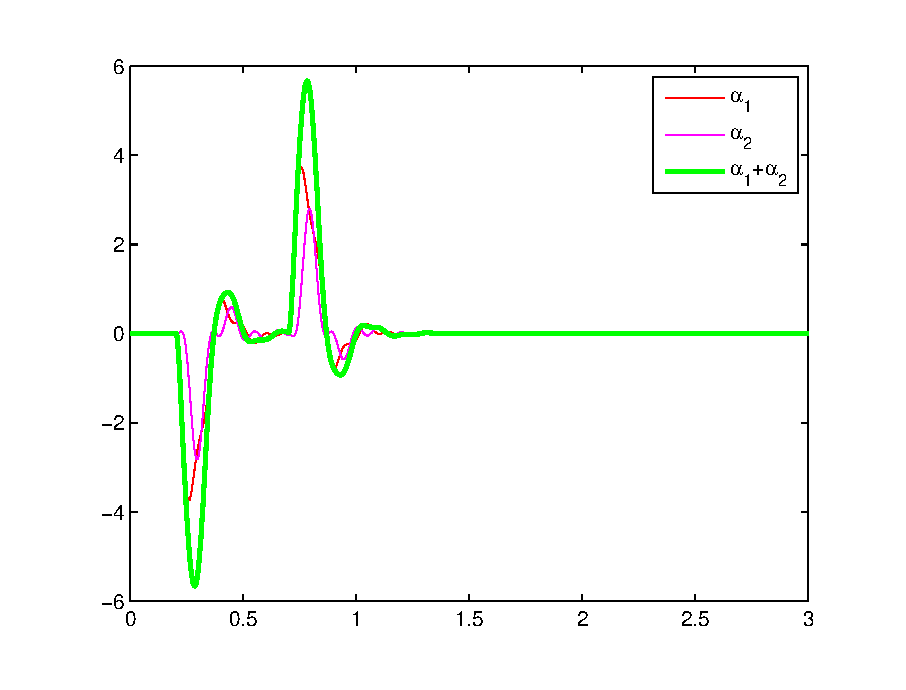
\includegraphics[width=.5\linewidth]{eps/lab_1/3DOF_response.eps}
              \caption{A plot of the response in the deflection angles, $\alpha_1$ and $\alpha_2$, due to a step input. The deflection angles are added together to compare the 2-DOF tip deflection to the 3-DOF tip deflection.}
              \label{fig:lab1_3DOF_response}
          \end{figure}
          \begin{figure}[htb!]
              \centering
              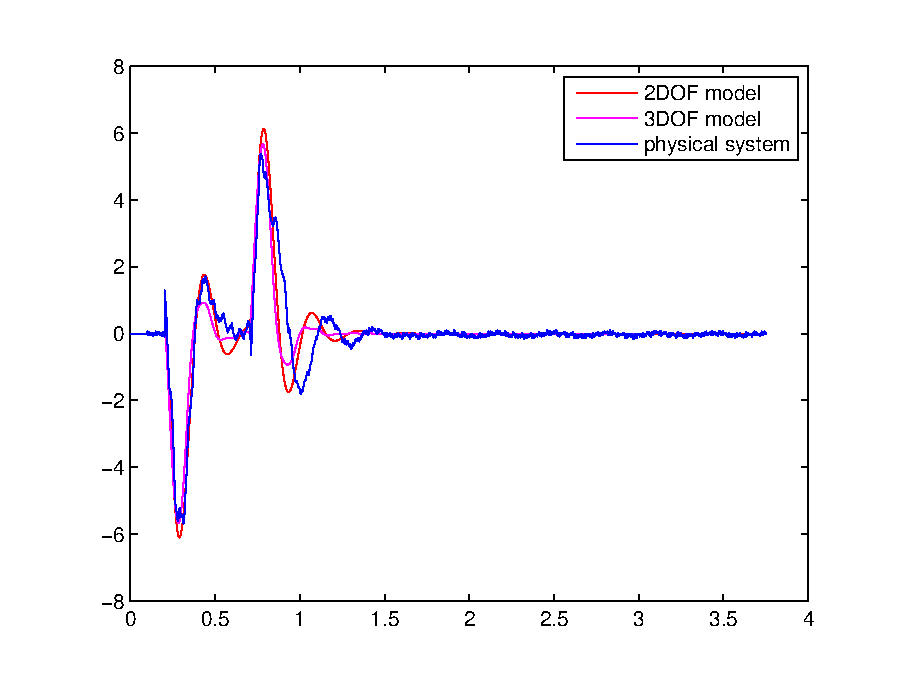
\includegraphics[width=.45\linewidth]{eps/lab_1/step_2to0_comparison.eps} \quad \quad
              \caption{A comparison of the 2-DOF model, 3-DOF model and physical system responses to a step input with initial value of 2.}
              \label{fig:lab1_comparison_step2to0}
          \end{figure}
\end{enumerate}

Please include plots of your 3-DOF model's responses to the three step input, plotting your comparison variable from Q9 with respect to time.
\newpage
\subsection{Deliverables}
To recap the lab objectives, this is what you need to include in your lab report to obtain full marks:
\begin{enumerate}
    \item prelab question (i) through (iii);
    \item the answers to questions Q2, Q5, Q6, Q8 and Q10 (include plots where requested);
\end{enumerate}
\textbf{Note: Save your lab report and have an electronic copy on-hand in all future labs, as you will need some of the values obtained in this lab to build upon this physical system.}

%----------------------------------------------------------------------------------------
%	Lab 2
%----------------------------------------------------------------------------------------
\newpage
\section{Lab 2: Controllability \& Observability of a Rotary Pendulum} \label{section:lab2}

\subsection{Introduction}\label{subsection:lab2_intro}
The purpose of this lab is to study a new system and to investigate the controllability and observability of this system. The prelab will focus on modelling a rotary pendulum using the same modern approach as was applied in \hyperref[section:lab1]{Lab~\ref{section:lab1}}. In the lab, you will move on to study whether the rotary pendulum is controllable or observable, using both a mathematical and an experimental approach.

\subsection{Prelab: Finding the Equations of Motion \& State-Space Representation}\label{subsection:lab2_prelab}
Rather than using first principles to model the rotary pendulum, you will use the Euler-Lagrange equations and follow the same treatment as in~\hyperref[subsection:lab1_prelab]{Section~\ref{subsection:lab1_prelab}} of Lab 1. Recall that the Lagrangian of a system is given by
\[
    L=T-V.
\]
For the rotary pendulum, you can define the generalized coordinate vector using the rotary shaft angle, $\theta$, and the pendulum rod angle, $\alpha$, as $q(t)^T=[\theta(t) \; \alpha(t)]$. To find the equations of motion for $\theta$ and $\alpha$, you may use the Euler-Lagrange equations:
\begin{equation*}\label{equation:lab2_lagrange_equns}
    \frac{d}{dt} \Bigg(\frac{\partial L}{\partial \dot{q_i}}\Bigg)  - \frac{\partial L}{\partial q_i} = Q_{q_i}.
\end{equation*}
As was done in \hyperref[section:lab1]{Lab~\ref{section:lab1}}, you may logic-out the generalized forces $Q_\theta$ and $Q_\alpha$: since the rotary shaft is actuated and the pendulum rod is not, and accounting for viscous friction, one can infer that $Q_\theta = \tau - B_r \dot{\theta} $ and $Q_\alpha = -B_p \dot{\alpha}$, where $\tau$ is the torque applied by the servo motor, and $B_r$, $B_p$ are the viscous damping coefficients for the rotary shaft and pendulum rod, respectively. As before, deriving the kinetic energy, $T$, and the potential energy, $V$, is not in the scope of this course. They are provided for this reason:
\begin{equation*}
    \begin{cases}
        T = \left(\frac{1}{2} m_p L_{r}^2 + \frac{1}{8} m_p L_{p}^2 - \frac{1}{8} m_p L_{p}^2 \cos^2(\alpha) + \frac{1}{2} J_r\right) \dot{\theta}^2 + \left(\frac{1}{2} J_p + \frac{1}{8} m_p L_{p}^2 \right) \dot{\alpha}^2 - \frac{1}{2} m_p L_p L_r \cos(\alpha) \dot{\theta} \dot{\alpha} \\
        V = \frac{1}{2} m_p L_p g \cos(\alpha)
    \end{cases}
\end{equation*}
where $J_p$, $m_p$, and $L_p$ are the moment of inertia about the centre of mass, mass, and length of the pendulum, respectively; $J_r$, $m_r$, and $L_r$ are the moment of inertia about the centre of mass, mass, and length of the rotary shaft, respectively; and $g$ is the acceleration due to gravity (on earth). Students wishing to find $T$ and $V$ on their own can do so using the model shown in Figure~\ref{fig:lab2_rotary_pendulum}. The complicated terms in $T$ come from the expression for the velocity of the pendulum at its centre of mass (you can find this velocity expression by using kinematics).

The final steps are left for you to complete $\dots$
\begin{figure}[htb!]
    \centering
    \subfigure[]{\includegraphics[width=.3\linewidth]{eps/lab_2/quanser.eps}}\quad \quad \quad \quad
    \subfigure[]{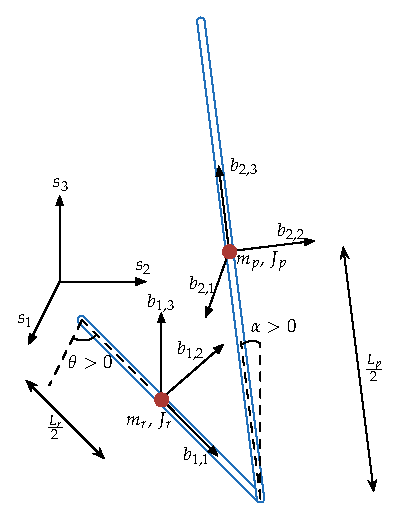
\includegraphics[height=0.5\linewidth,keepaspectratio]{eps/lab_2/rotary_pendulum_edit.eps}}
    \caption{(a) Physical rotary pendulum system~\cite{Q-Flex-Beam}; (b) model of the physical system with two rigid bodies connected together, where rigid body 1 (rotary shaft) rotates in the horizontal plane and rigid body 2 (pendulum rod) rotates in the vertical plane. The reference coordinate axes are shown by $\{s_1,s_2,s_3\}$, and the body coordinate axes for rigid bodies 1 and 2 are shown by $\{b_{1,1},b_{1,2}, b_{1,3}\}$ and $\{b_{2,1},b_{2,2},b_{2,3}\}$, respectively. The centres of mass for bodies 1 and 2 are shown in red; the horizontal rotation angle, $\theta$, the vertical rotation angle, $\alpha$, are shown. Important distances are labelled.}
    \label{fig:lab2_rotary_pendulum}
\end{figure}

\subsubsection{Prelab Questions:}\label{subsubsection:lab2s_prelab}
\begin{enumerate}
    \item What is the equation of motion for generalized coordinate $\theta$?\\
          \drew{Answer: it is
              \begin{align*}
                   & \left(m_p L_{r}^{2} + \frac{1}{4} m_p L_{p}^{2} - \frac{1}{4} m_p L_{p}^{2} \cos^2(\alpha) + J_r\right) \ddot{\theta} - \frac{1}{2} m_p L_p L_r \cos(\alpha) \ddot{\alpha} \\
                   & + \frac{1}{2} m_p L_{p}^{2} \sin(\alpha)\cos(\alpha) \dot{\theta}\dot{\alpha} + \frac{1}{2}m_p L_p L_r \sin(\alpha) \dot{\alpha}^{2} = \tau - B_r \dot{\theta}
              \end{align*}
              This is obtained via the Euler-Lagrange equation. One calculates:
              \[
                  \begin{cases}
                      \pder{L}{\theta}=0                                                                                                                                                       \\
                      \pder{L}{\dot{\theta}}=\left( m_pL_r^2 +\frac{1}{4} m_p L_p^2-\frac{1}{4}m_pL_p^2\cos^2(\alpha)+J_r\right)\dot{\theta} - \frac{1}{2} m_pL_pL_r\cos{(\alpha)}\dot{\alpha} \\
                      \frac{d}{dt} \left(\pder{L}{\dot{\theta}}\right)= \left(m_pL_r^2 +\frac{1}{4}m_pL_p^2-\frac{1}
                      {4}m_pL_p^2\cos^2(\alpha)+J_r\right)\ddot{\theta} + \frac{1}{2}m_pL_p^2\sin{(\alpha)}\cos{(\alpha)} \dot{\alpha}\dot{\theta}                                             \\+ \frac{1}{2}m_pL_pL_r\sin{(\alpha)}\dot{\alpha}^2-\frac{1}{2}m_pL_pL_r\cos{(\alpha)}\ddot{\alpha} \\
                  \end{cases}
              \]
              which yields the above EOMs.}
    \item What is the equation of motion for generalized coordinate $\alpha$?\\
          \drew{Answer: it is
              \begin{align*}
                   & -\frac{1}{2} m_p L_p L_r \cos(\alpha) \ddot{\theta} + \left(J_p + \frac{1}{4} m_p L_{p}^{2}\right)\ddot{\alpha} - \frac{1}{4} m_p L_{p}^{2} \sin(\alpha)\cos(\alpha) \dot{\theta}^{2} \\
                   & - \frac{1}{2} m_p L_{p} g \sin(\alpha) = - B_p \dot{\alpha}
              \end{align*}
              This is obtained via the Lagrange calculations. One calculates:
              \[
                  \begin{cases}
                      \pder{L}{\alpha}=\frac{1}{4}m_pL_p^2\cos{(\alpha)}\sin{(\alpha)}\dot{\theta}^2+\frac{1}{2}m_pL_pL_r\sin{(\alpha)}\dot{\theta}\dot{\alpha}+ \frac{1}{2}m_pL_pg\sin{\alpha} \\
                      \pder{L}{\dot{\alpha}}= \left(J_p+\frac{1}{4}m_pL_p^2\right)\dot{\alpha}-\frac{1}{2}m_pL_pL_r\cos{(\alpha)}\dot{\theta}                                                   \\
                      \frac{d}{dt} \left(\pder{L}{\dot{\alpha}}\right)= \left(J_p+\frac{1}{4}m_pL_p^2\right)\ddot{\alpha}+\frac{1}{2}m_pL_pL_r\sin{(\alpha)}\dot{\theta}\dot{\alpha}-\frac{1}{2}m_pL_pL_r\cos{(\alpha)} \ddot{\theta}
                  \end{cases}
              \]
              which yields the above EOMs.}
    \item What does it mean for a system to be controllable? What does it mean for a system to be observable?\\
          \drew{Answer:\\
              \textbf{Controllability:} We say that a system is controllable if it is possible to steer the state of a system from any initial value to any desired value in finite time by using an admissible control input.\\
              \textbf{Observability:} We say that a system is observable if the initial value of the state can be recovered by using the state output trajectory (i.e., the output over time except at time $t=0$).}
\end{enumerate}

\subsection{Linearization}\label{subsubsection:lab2_linearize}
You may notice that your EOMs that you calculated in the prelab are nonlinear equations. In this section, you will linearize these equations about a set equilibrium point.

\begin{enumerate}
    \item[Q1:] What is the \emph{linearized} equation of motion for generalized coordinate $\theta$ about equilibrium point $\theta_0 = 0$ and $\alpha_0 = \pi$?\\
          \textbf{Hint:} Recall that to linearize a multivariate function $f$ of variables $z^T = [\theta \; \alpha \; \dot{\theta} \; \dot{\alpha} \; \ddot{\theta} \; \ddot{\alpha}]$ around an equilibrium point $z_{0}^T = [\theta_0 \; \alpha_0 \; \dot{\theta}_0 \; \dot{\alpha}_0 \; \ddot{\theta}_0 \; \ddot{\alpha}_0]$, you compute
          \[
              f_\text{lin} = f(z_0) + \left(\frac{\partial f(z)}{\partial \theta}\right) \bigg|_{z_0}  (\theta - \theta_0) +  \left(\frac{\partial f(z)}{\partial \alpha}\right) \bigg|_{z_0}  (\alpha - \alpha_0) + \dots +  \left(\frac{\partial f(z)}{\partial \ddot{\alpha}}\right) \bigg|_{z_0}  (\ddot{\alpha} - \ddot{\alpha}_0).
          \]
          \drew{Answer: it is
              \[
                  \left(m_p L_{r}^{2} + J_r\right) \ddot{\theta} + \frac{1}{2} m_p L_p L_r \ddot{\alpha} = \tau - B_r \dot{\theta}.
              \]
              This is by virtue of the linearization technique explained above. Note that the righthand side of the EOM are already linear. One computes the following, where $f$ is equal to the lefthand side of the EOM:
              \[
                  \begin{cases}
                      f(z_0) = 0                                                                                                                                                    \\
                      \pder{f}{\theta}\big|_{z_0} (\theta-0) = 0                                                                                                                    \\
                      \pder{f}{\alpha}\big|_{z_0} (\alpha-\pi) = 0                                                                                                                  \\
                      \pder{f}{\dot{\theta}}\big|_{z_0} (\dot{\theta}-0) = 0                                                                                                        \\
                      \pder{f}{\dot{\alpha}}\big|_{z_0} (\dot{\alpha}-0)= 0                                                                                                         \\
                      \pder{f}{\dot{\theta}}\big|_{z_0} (\ddot{\theta}-0)= \left(m_pL_r^2-\frac{1}{4}m_pL_p^2\cos^2(\alpha)+\frac{1}{4}m_pL_p^2+J_r \right)\big|_{z_0}\ddot{\theta} \\
                      \pder{f}{\dot{\alpha}}\big|_{z_0} (\ddot{\alpha}-0)= \left(-\frac{1}{2}m_pL_pL_r\cos{(\alpha)}\right)\big|_{z_0} \ddot{\alpha}.                               \\
                  \end{cases}
              \]
          }
    \item[Q2:] What is the \emph{linearized} equation of motion for generalized coordinate $\alpha$ about equilibrium point $\theta_0 = 0$ and $\alpha_0 = \pi$? \textbf{Note:} After doing this linearization, you should have a $(\alpha-\pi)$ term; change this term to $\alpha$ for simplicity. \\
          \drew{Answer: it is
              \[
                  \frac{1}{2} m_p L_p L_r \ddot{\theta} + \left(J_p + \frac{1}{4} m_p L_{p}^{2}\right)\ddot{\alpha} + \frac{1}{2} m_p L_{p} g \alpha = - B_p \dot{\alpha}
              \]
              This is by virtue of the linearization technique explained above. Note that the righthand side of the EOM are already linear. One computes the following, where $f$ is equal to the lefthand side of the EOM:
              \[
                  \begin{cases}
                      f(z_0) = 0                                                                                              \\
                      \pder{f}{\theta}\big|_{z_0} (\theta-0) = 0                                                              \\
                      \pder{f}{\alpha}\big|_{z_0} (\alpha-\pi) = \frac{1}{2}m_pL_pg(\alpha-\pi)                               \\
                      \pder{f}{\dot{\theta}}\big|_{z_0} (\dot{\theta}-0) = 0                                                  \\
                      \pder{f}{\dot{\alpha}}\big|_{z_0} (\dot{\alpha}-0)= 0                                                   \\
                      \pder{f}{\dot{\theta}}\big|_{z_0} (\ddot{\theta}-0)= \frac{1}{2}m_pL_pL_r\ddot{\theta}                  \\
                      \pder{f}{\dot{\alpha}}\big|_{z_0} (\ddot{\alpha}-0)= \left(J_p+\frac{1}{4}m_pL_p^2\right)\ddot{\alpha}. \\
                  \end{cases}
              \]
              Then, one replaces $(\alpha-\pi)$ by $\alpha$, to simplify things. This can be done since the system is linear.
          }
    \item[Q3:] What is your state-space model, including symbolic matrices $A$ and $B$?\\
          \textbf{Hint:} Write the linearized EOMs in matrix form, i.e.,
          \[
              \left[\begin{array}{c c}
                      e_{11} & e_{12} \\
                      e_{21} & e_{22}
                  \end{array}\right]
              \left[\begin{array}{c}
                      \ddot{q}_{1} \\
                      \ddot{q}_{2}
                  \end{array}\right] +
              \left[\begin{array}{c c}
                      f_{11} & f_{12} \\
                      f_{21} & f_{22}
                  \end{array}\right]
              \left[\begin{array}{c}
                      \dot{q}_{1} \\
                      \dot{q}_{2}
                  \end{array}\right] +
              \left[\begin{array}{c c}
                      g_{11} & g_{12} \\
                      g_{21} & g_{22}
                  \end{array}\right]
              \left[\begin{array}{c}
                      q_{1} \\
                      q_{2}
                  \end{array}\right] =
              \left[\begin{array}{c}
                      \tau_1 \\
                      \tau_2
                  \end{array}\right],
          \]
          and group all non double-derivative terms to the right. Now, let
          \[J_T = det
              \left[\begin{array}{c c}
                      e_{11} & e_{12} \\
                      e_{21} & e_{22}
                  \end{array}\right],
          \]
          recalling that the determinant of a matrix $M \in \mathbb{R}^{2\times2}$ is the product of its entries on the diagonal subtracted by the product of its entries on the off-diagonal. You can now explicitly solve for $\left[\begin{array}{c}
                      \ddot{\theta} \\
                      \ddot{\alpha}
                  \end{array}\right]$ and put it in a relatively compact form. You should let your state be
          \[
              x(t) =
              \left[\begin{array}{c}
                      \theta(t)       \\
                      \alpha(t)       \\
                      \dot{\theta}(t) \\
                      \dot{\alpha}(t)
                  \end{array}\right]
          \]
          when writing our your state-space representation.\\
          \drew{Answer: the state-space representation is
              \begin{align*}
                   & \left[\begin{array}{c}
                          \dot{\theta}(t)  \\
                          \dot{\alpha}(t)  \\
                          \ddot{\theta}(t) \\
                          \ddot{\alpha}(t)
                      \end{array}\right] = \frac{1}{J_T}
                  \left[\begin{array}{c c c c}
                          0 & 0                                                     & J_T                                            & 0                                  \\
                          0 & 0                                                     & 0                                              & J_T                                \\
                          0 & \frac{1}{4} m_{p}^2 L_{p}^2 L_r g                     & -\left(J_p + \frac{1}{4} m_p L_{p}^2\right)B_r & \frac{1}{2} m_p L_p L_r B_p        \\
                          0 & -\frac{1}{2} m_p L_p g \left(J_r + m_p L_{r}^2\right) & \frac{1}{2} m_p L_p L_r B_r                    & -\left(J_r + m_p L_{r}^2\right)B_p
                      \end{array}\right]
                  \left[\begin{array}{c}
                          \theta(t)       \\
                          \alpha(t)       \\
                          \dot{\theta}(t) \\
                          \dot{\alpha}(t)
                      \end{array}\right]                    \\
                   & + \frac{1}{J_T}
                  \left[\begin{array}{c}
                          0                             \\
                          0                             \\
                          J_p + \frac{1}{4} m_p L_{p}^2 \\
                          -\frac{1}{2} m_p L_p L_r
                      \end{array}\right] \tau
              \end{align*}}
\end{enumerate}

\subsection{Validity of Linearization}\label{lab2:linearization_validity}
In this section, you will observe in what domain your linearization of the EOMs from the Prelab is valid. To do this, you will compare the physical system's and your state-space model's response to various step inputs that will increase in magnitude, similar to the approach taken in \hyperref[subsubsection:lab1_modelvalidation]{Section~\ref{subsubsection:lab1_modelvalidation}} of Lab 1. To do this, you must first evaluate your symbolic matrices $A$ and $B$, thus the following values are given:
\[
    \begin{cases}
        B_p = 0.0 \; \frac{N\cdot s}{m}   \\
        B_r = 0.137 \; \frac{N\cdot s}{m} \\
        L_p = 0.3365 \; m                 \\
        L_r = 0.2159 \; m                 \\
        m_p = 0.1270 \; kg                \\
        m_r = 0.2570 \; kg
    \end{cases}
\]
Recall that the moment of inertia of a thin rod about its centre of mass is $J = \frac{1}{12} m L^2$ (use this to find $J_p$ and $J_r$). Again, you must transform the state-space model from your prelab in terms of voltage rather than in terms of torque (as was done in Lab 1). Follow these steps in sequence to do so:
\begin{enumerate}
    {\indentitem \item[Step 1:] let matrix entry $A(3,3) = A(3,3) - \frac{K_{g}^2 k_t k_m}{R_m} B(3)$, where $K_g=70$ is the total gear ratio for your setup, $k_t=0.0077$ is the servo motor torque constant, $k_m = 0.0077$ is the motor back-EMF const   $R_m=2.6$ is the motor armature resistance;} \\
          {\indentitem \item[Step 2:] let matrix entry $A(4,3) = A(4,3) - \frac{K_{g}^2 k_t k_m}{R_m} B(4)$;} \\
          {\indentitem \item[Step 3:] only now should you modify $B$ to $B = \frac{K_g k_t}{R_m} B$.}
\end{enumerate}
We've prepared a MATLAB script for you to speed up the process: open \textbf{lab2\_statespace\_student}, input your symbolic matrices that you computed in your prelab, and run the script to evaluate your state-space matrices $A$ and $B$.
\begin{enumerate}[Question]
    \item[Q4:] What are the numerically-evaluated matrices $A$ and $B$ for the state-space model?\\
          \drew{Answer: You should get
              \[
                  A =
                  \left[\begin{array}{c c c c}
                          0 & 0       & 1      & 0       \\
                          0 & 0       & 0      & 1       \\
                          0 & 81.38   & -93.49 & 0.0038  \\
                          0 & -122.03 & 89.97  & -0.0058 \\
                      \end{array}\right]
              \]
              and
              \[
                  B =
                  \left[\begin{array}{c}
                          0       \\
                          0       \\
                          83.6412 \\
                          -80.4864
                      \end{array}\right].
              \]
          }
    \item[Q5:] Given that the physical system's sensors are limited to reading the rotor shaft angle and the pendulum angle, what are the numerical matrices $C$ and $D$ for the state-space model?\\
          \drew{Answer: You should get
              \[
                  C =
                  \left[\begin{array}{c c c c}
                          1 & 0 & 0 & 0 \\
                          0 & 1 & 0 & 0
                      \end{array}\right]
              \]
              and
              \[
                  D =
                  \left[\begin{array}{c}
                          0 \\
                          0
                      \end{array}\right],
              \]
              which can be discerned from the state-space equation $y = Cx + Du$.
          }
\end{enumerate}
Now that you have a state-space representation for the physical system, you can start constructing a Simulink model that will interact with the Quanser SRV02 servo motor, which you will use to investigate the domain of validity, controllability \& observability for your linearized model. Please \textbf{save all of your MATLAB and Simulink files} as you may need to consult them in future labs.
\subsubsection{Setting up the Rotary Pendulum}\label{subsubsection:lab2_setup}
First, let us assemble and wire the physical system. Examine the close-up assembly shown in Figure~\ref{fig:lab1a_assembly}, and replicate this at your workstation. Note that the high-gear configuration is used here. Use the wiring diagram shown in Figure~\ref{fig:lab1a_wiring} to connect the rotary pendulum to a power source and the data acquisition board.
\begin{figure}[htb!]
    \centering
    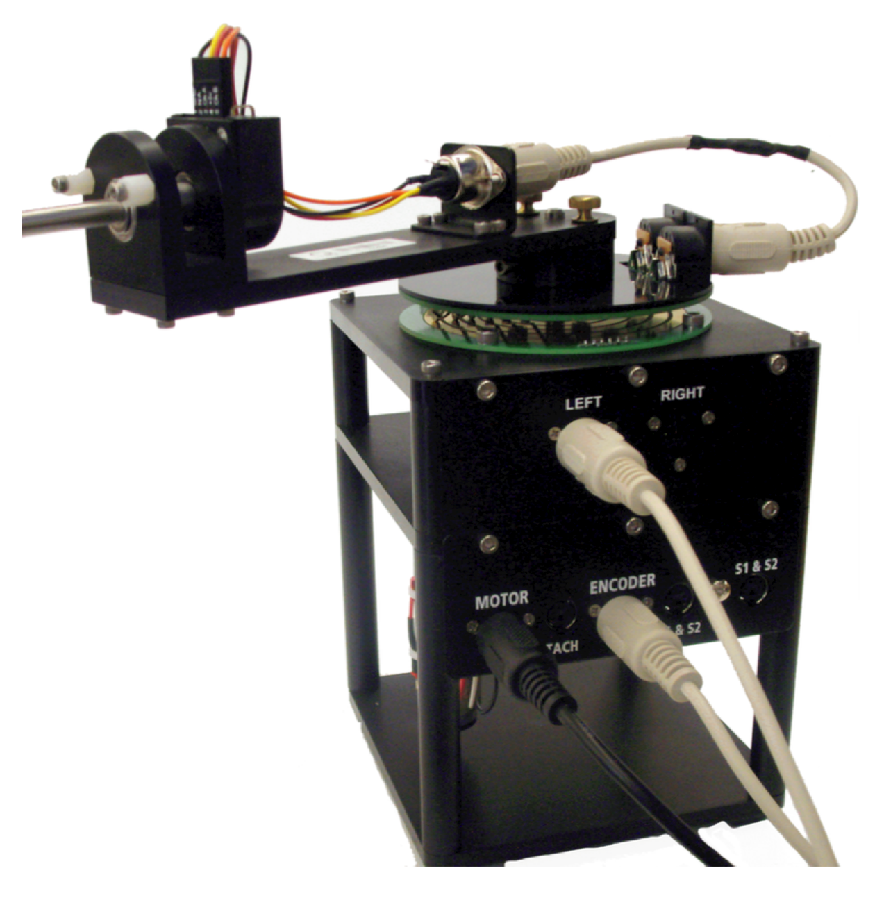
\includegraphics[width=.3\linewidth]{eps/lab_2/assembly.eps}
    \caption{A close-up of the assembly of the rotary pendulum module and the Quanser SRV02 plant~\cite{Q-Flex-Beam}.}
    \label{fig:lab1a_assembly}
\end{figure}
\begin{figure}[htb!]
    \centering
    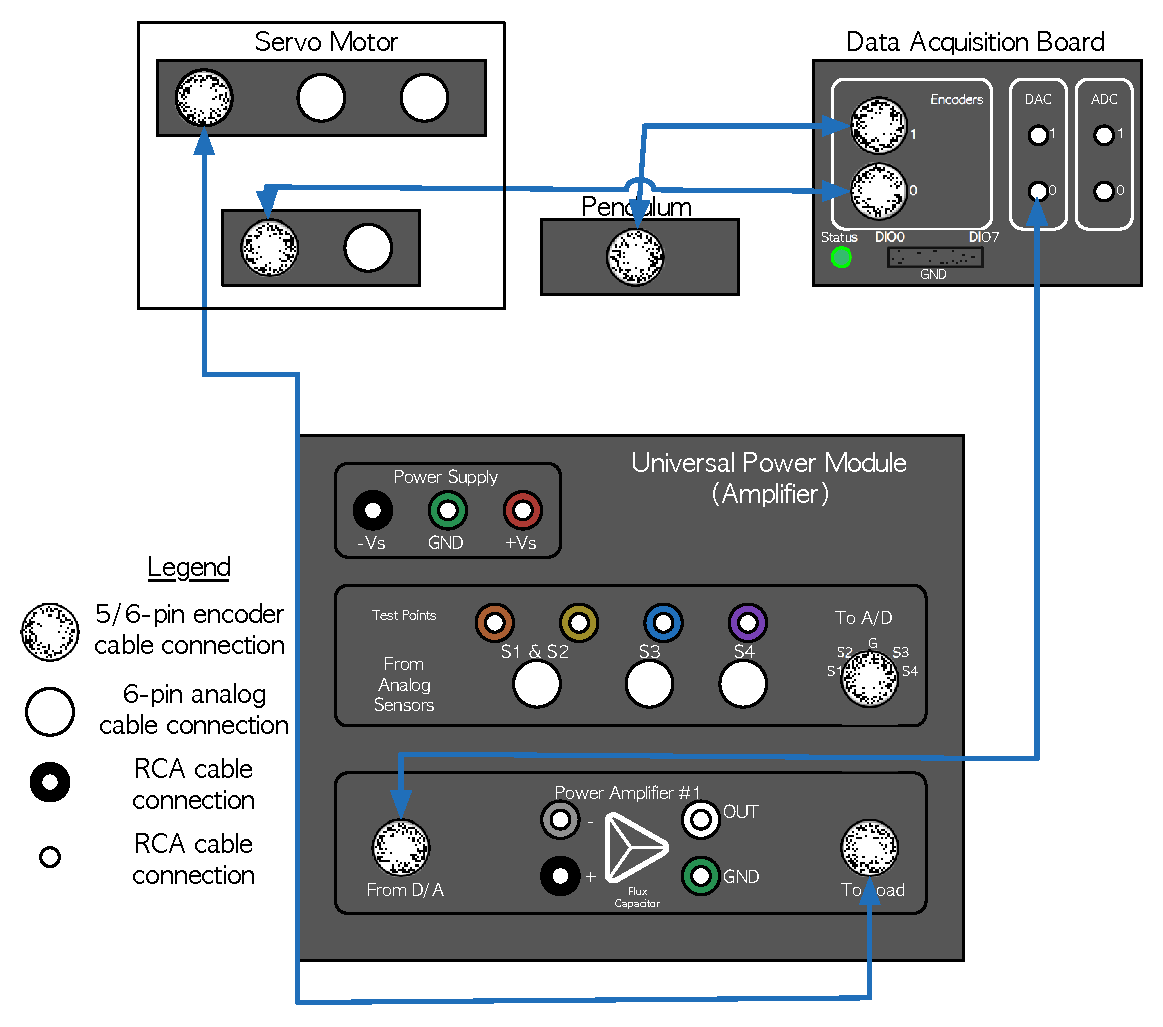
\includegraphics[width=.7\linewidth]{eps/lab_2/wiring.eps}
    \caption{A wiring diagram for the Quanser SRV02 and rotary pendulum module.}
    \label{fig:lab1a_wiring}
\end{figure}

\textbf{Note:} The power amplifier must be turned on before you can experiment with the physical system. The power switch is located at the back of the amplifier (good luck finding it). Make sure to turn off the power amplifier before you leave the lab.
\subsubsection{Simulink Model}
You will be simulating various inputs and initial condition combinations with both your state-space model and the physical system. By now, you should be comfortable with modifying Simulink models. Open the file \textbf{validation\_model.mdl} and modify it to incorporate your state-space model, as shown in Figure~\ref{fig:lab2_simulink_model}.
\begin{figure}[htb!]
    \centering
    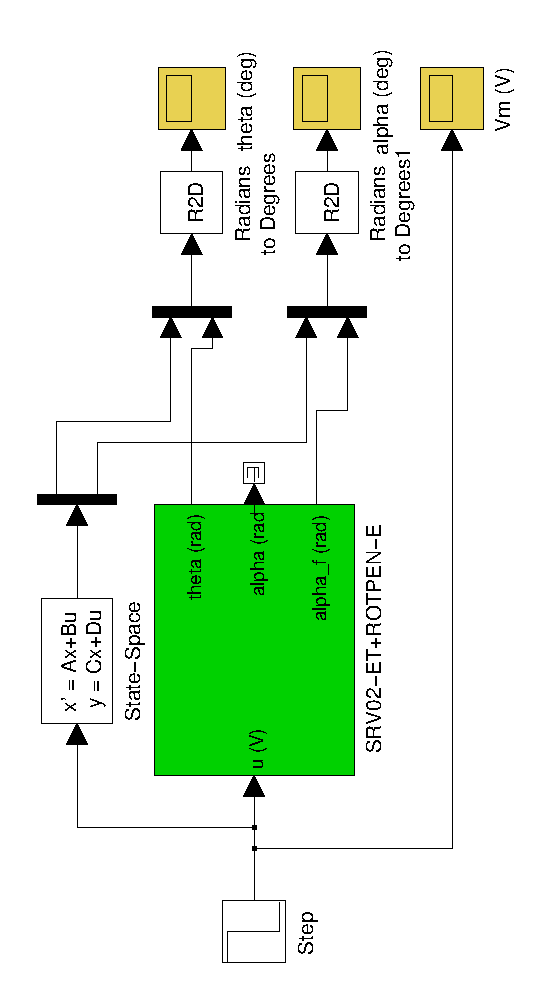
\includegraphics[width=.4\linewidth, angle=270]{eps/lab_2/simulink_model.eps}
    \caption{A Simulink model that interacts with the rotary pendulum system and incorporates the state-space model~\cite{Q-Flex-Beam}.}
    \label{fig:lab2_simulink_model}
\end{figure}

Repeat the steps outlined in \hyperref[subsubsection:lab1_modelvalidation]{Section~\ref{subsubsection:lab1_modelvalidation}} of Lab~1 to obtain time plots of the responses of the physical system and the state-space model. This time, use step inputs with initial values of 0.3, 0.6 and 0.9, and stop running the model after about 5 seconds for all trials.
\begin{enumerate}[Question]
    \item[Q6:] Plot the responses of the physical system and the state-space model to three different step function with initial values of 0.3, 0.6 and 0.9 (leaving the Step time at 0.5 seconds). From these three time plots, what can you conclude about the domain of validity of your linearization?\\
          \drew{Answer: As is shown in the first plot, the state-space model does a pretty good job at modelling the physical system for a step input with initial value of 0.3. The physical system's overall damping is less for the pendulum but higher for the rotor base. In the second and third plots, one can see that the linearized system is less accurate. This is because the domain of validity for the linearization is small around the linearization about $\alpha = \pi$, so perturbing the pendulum angle more from this equilibrium makes the model less accurate. Note that the rotor base state-space dynamics seems to be underdamped whereas the pendulum state-space dynamics seems to be overdamped; the underdamped and over damped effects worsen with a larger step input.
              \begin{figure}[htb!]
                  \centering
                  \subfigure[]{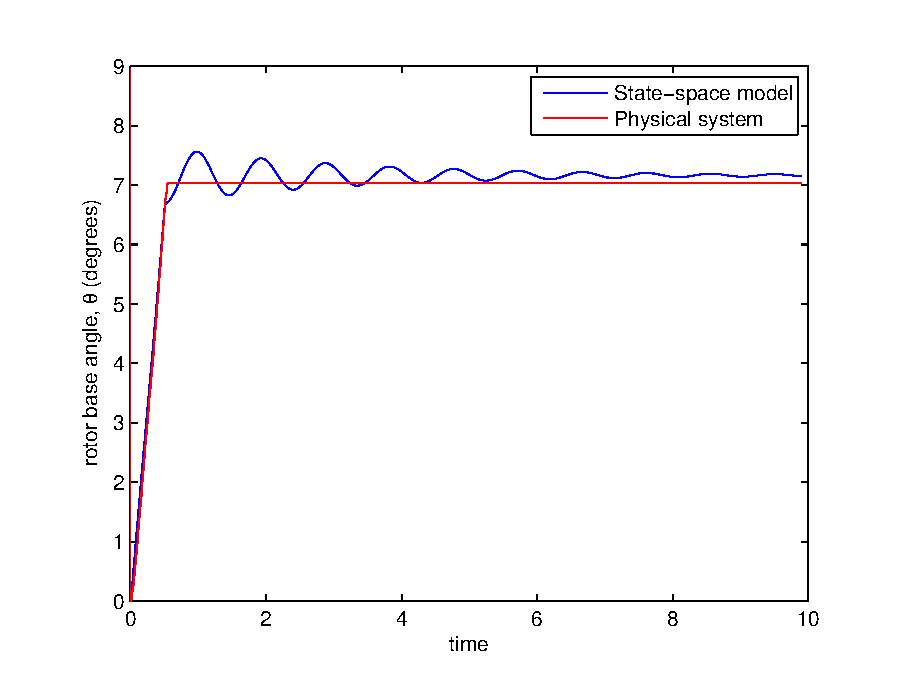
\includegraphics[width=.4\linewidth]{eps/lab_2/model_validation_3to0_theta.eps}} \quad \quad
                  \subfigure[]{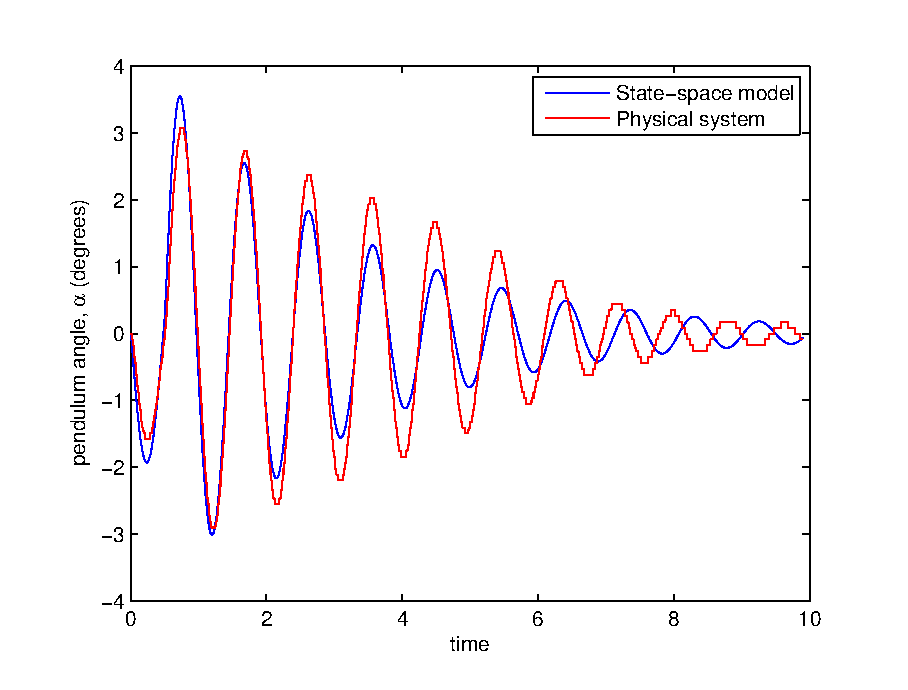
\includegraphics[width=.4\linewidth]{eps/lab_2/model_validation_3to0_alpha.eps}}
                  \caption{Responses of the physical rotary pendulum system and the linearized state-space model to a step input with initial value of 0.3, step time of 0.5 and final value of 0, where (a) is the rotor base angle and (b) is the pendulum angle.}
              \end{figure}
              \begin{figure}[htb!]
                  \centering
                  \subfigure[]{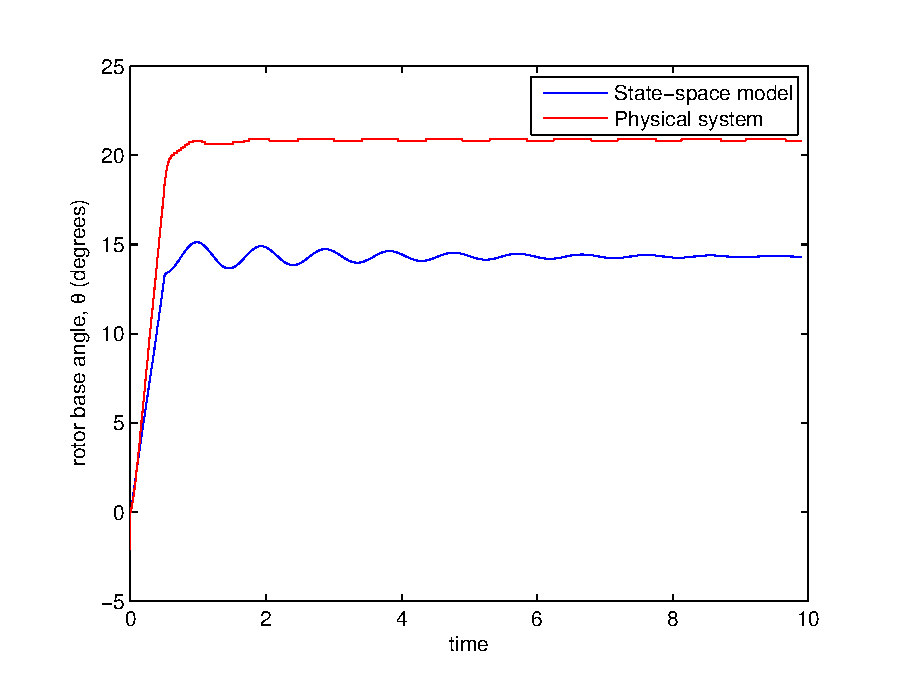
\includegraphics[width=.4\linewidth]{eps/lab_2/model_validation_6to0_theta.eps}} \quad \quad
                  \subfigure[]{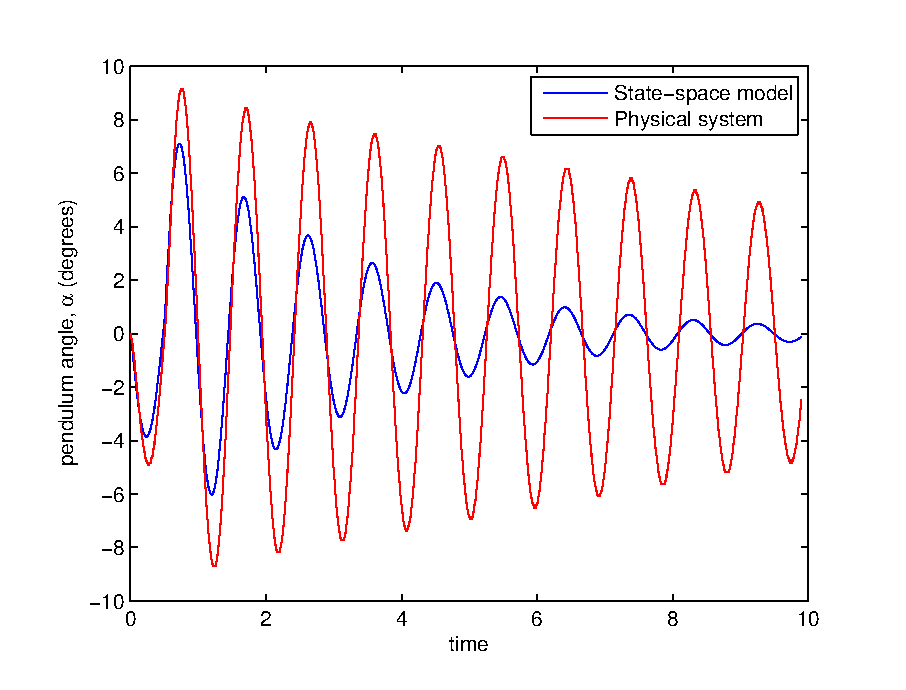
\includegraphics[width=.4\linewidth]{eps/lab_2/model_validation_6to0_alpha.eps}}
                  \caption{Responses of the physical rotary pendulum system and the linearized state-space model to a step input with initial value of 0.6}
              \end{figure}
              \begin{figure}[htb!]
                  \centering
                  \subfigure[]{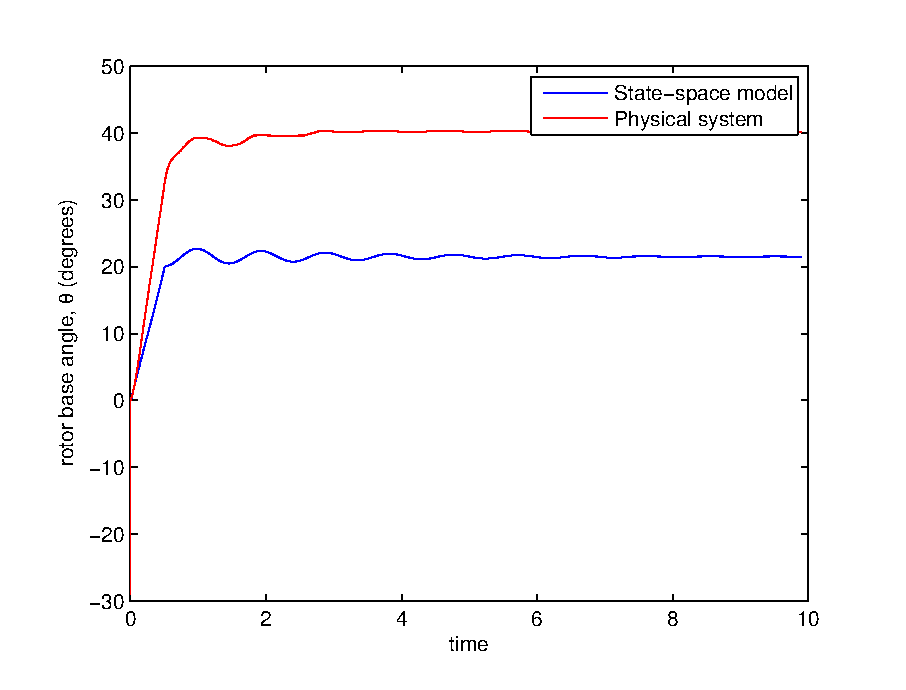
\includegraphics[width=.4\linewidth]{eps/lab_2/model_validation_9to0_theta.eps}} \quad \quad
                  \subfigure[]{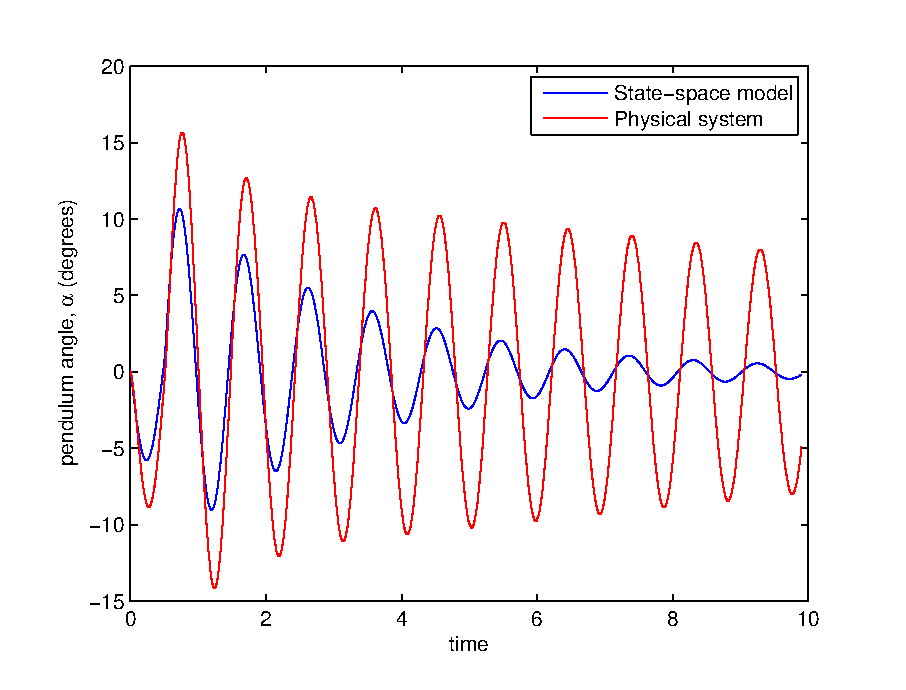
\includegraphics[width=.4\linewidth]{eps/lab_2/model_validation_9to0_alpha.eps}}
                  \caption{Responses of the physical rotary pendulum system and the linearized state-space model to a step input with initial value of 0.9.}
              \end{figure}
          }
\end{enumerate}
\subsection{Controllability \& Observability}\label{subsection:lab2_math_approach}
In this section, you will use your evaluated state-space matrices to find $\mathcal{C}_{(A,B)}$ and $\mathcal{O}_{(A,C)}$. Afterwards, you can determine whether the rotary pendulum system is controllable and observable.
\begin{enumerate}[Question]
    \item[Q7:] What are the controllability and observability matrices for the linear state-space representation of the rotary pendulum? Is the rotary pendulum system controllable? Is it observable?\\
          \drew{Answer: You should get
              \[
                  \mathcal{C}_{(A,B)} =
                  \left[\begin{array}{c c c c}
                          0      & 83.64    & -7820.62   & 724693.53    \\
                          0      & -80.48   & 7525.80    & -693855.77   \\
                          83.64  & -7820.62 & 724693.53  & -67147820.71 \\
                          -80.48 & 7525.80  & -693855.77 & 64287501.90
                      \end{array}\right]
              \]
              and \\
              \[
                  \mathcal{O}_{(C,A)} =
                  \left[\begin{array}{c c c c}
                          1 & 0        & 0        & 0       \\
                          0 & 1        & 0        & 0       \\
                          0 & 0        & 1        & 0       \\
                          0 & 0        & 0        & 1       \\
                          0 & 81.38    & -93.49   & 0.0038  \\
                          0 & -122.03  & 89.97    & -0.0058 \\
                          0 & -7609.66 & 8742.27  & 81.02   \\
                          0 & 7322.89  & -8412.72 & -121.68
                      \end{array}\right].
              \]
              The system is both controllable and observable as
              \[
                  \text{rank}(\mathcal{C}_{(A,B)}) = \text{rank}(\mathcal{O}_{(A,C)})=4.
              \]}
    \item[Q8:] The encoder that reads the rotor base angle suddenly breaks. With this change, is the rotary pendulum system controllable? Is it observable? If the system is uncontrollable or unobservable, what (initial) states can we not (recover) access, and what does this mean in regards to our physical system?\\
          \textbf{Hint:} What is in the null space of $\mathcal{C}_{(A,B)}$, $\mathcal{O}_{(A,C)}$, and what does this tell us about the system?\\
          \drew{Answer: the controllability matrix remains the same, and thus the system is still controllable. The state-space matrix $C$ becomes
              \[
                  C =
                  \left[\begin{array}{c c c c}
                          0 & 0 & 0 & 0 \\
                          0 & 1 & 0 & 0
                      \end{array}\right],
              \]
              which in turn changes the observability matrix to
              \[
                  \mathcal{O}_{(C,A)} =
                  \left[\begin{array}{c c c c}
                          0 & 0       & 0        & 0       \\
                          0 & 1       & 0        & 0       \\
                          0 & 0       & 0        & 0       \\
                          0 & 0       & 0        & 1       \\
                          0 & 0       & 0        & 0       \\
                          0 & -122.03 & 89.97    & -0.0058 \\
                          0 & 0       & 0        & 0       \\
                          0 & 7322.89 & -8412.72 & -121.68 \\
                      \end{array}\right],
              \]
              which has rank 3. Thus the system is not observable. Note that the null space of $\mathcal{O}_{(C,A)}$ is
              \[
                  \mathrm{Null}(\mathcal{O}_{(C,A)}) =
                  \left\{\left[\begin{array}{c}
                          1 \\
                          0 \\
                          0 \\
                          0
                      \end{array}\right]\right\}
              \]
              This means that if your rotor shaft encoder is damaged, you cannot recover the initial rotor shaft angle by using output data.
          }
    \item[Q9:] The encoder that reads the pendulum angle suddenly breaks. With this change, is the rotary pendulum system controllable? Is it observable? If the system is uncontrollable or unobservable, what (initial) states can we not (recover) access, and what does this mean in regards to our physical system?\\
          \drew{Answer: the state-space matrix $C$ becomes
              \[
                  C =
                  \left[\begin{array}{c c c c}
                          1 & 0 & 0 & 0 \\
                          0 & 0 & 0 & 0
                      \end{array}\right],
              \]
              which in turn changes the observability matrix to
              \[
                  \mathcal{O}_{(C,A)} =
                  \left[\begin{array}{c c c c}
                          1 & 0        & 0       & 0      \\
                          0 & 0        & 0       & 0      \\
                          0 & 0        & 1       & 0      \\
                          0 & 0        & 0       & 0      \\
                          0 & 81.38    & -93.49  & 0.0038 \\
                          0 & 0        & 0       & 0      \\
                          0 & -7609.66 & 8742.27 & 81.02  \\
                          0 & 0        & 0       & 0
                      \end{array}\right],
              \]
              which has rank 4. Thus the system is still observable. It is also still controllable, as the controllability matrix remains the same. This means that one can estimate the pendulum angle state trajectory by simply observing the system inputs and outputs and by building a state observer.}
\end{enumerate}

\subsection{Deliverables}
To recap the lab objectives, this is what you need to include in your lab report to obtain full marks:
\begin{enumerate}
    \item prelab question (i) and (ii);
    \item the answers to questions Q1 through Q3 and Q6 through Q9 (include plots where requested);
\end{enumerate}
\textbf{Note: Save your lab report and have an electronic copy on-hand in all future labs, as you will need some of the values obtained in this lab to build upon this physical system.}
%----------------------------------------------------------------------------------------
%	Lab 3
%----------------------------------------------------------------------------------------
\newpage
\section{Lab 3: Stability, Feedback Control \& Luenberger Observer for Balancing an Inverted Rotary Pendulum} \label{section:lab3}

\subsection{Introduction}\label{subsection:lab3_intro}
The purpose of this lab is to study another equilibrium of the rotary pendulum system and to develop a control technique that balances the pendulum around this equilibrium using partial state feedback and a linear observer. The prelab focuses on the linearization of the EOMs for the rotary pendulum about the equilibrium point where the pendulum is completely inverted, and also focuses on analyzing the stability of the system at this equilibrium point. In the lab, you will first use full state feedback and pole placement techniques to develop a controller that balances the inverted pendulum. Then, you will carry out the same task for the case where you do not have access to the full state information. To do this, you will develop a Luenberger observer to estimate the states that you do not have access to and you will use the estimated states to develop a controller that balances the inverted pendulum.
\begin{figure}[htb!]
    \centering
    \includegraphics[width=.3\linewidth]{eps/lab_3/quanser.eps}
    \caption{Qanser SRV02 with pendulum module, shown in an inverted orientation~\cite{Q-Flex-Beam}.}
    \label{fig:lab3_plant}
\end{figure}
\subsection{Prelab: Linearization, State-Space Representation \& Stability Analysis}\label{subsection:lab3_prelab}
\begin{enumerate}
    \item What is the \emph{linearized} equation of motion for generalized coordinate $\theta$ about equilibrium point $\theta_0 = 0$ and $\alpha_0 = 0$? You'll need to refer to your answers for the EOMs of the rotary pendulum from \hyperref[subsection:lab2_prelab]{Section~\ref{subsection:lab2_prelab}} in Lab 2.\\
          \textbf{Hint:} Recall that to linearize a multivariate function $f$ of variables $z^T = [\theta \; \alpha \; \dot{\theta} \; \dot{\alpha} \; \ddot{\theta} \; \ddot{\alpha}]$ around an equilibrium point $z_{0}^T = [\theta_0 \; \alpha_0 \; \dot{\theta}_0 \; \dot{\alpha}_0 \; \ddot{\theta}_0 \; \ddot{\alpha}_0]$, you compute
          \[
              f_\text{lin} = f(z_0) + \left(\frac{\partial f(z)}{\partial \theta}\right) \bigg|_{z_0}  (\theta - \theta_0) +  \left(\frac{\partial f(z)}{\partial \alpha}\right) \bigg|_{z_0}  (\alpha - \alpha_0) + \dots +  \left(\frac{\partial f(z)}{\partial \ddot{\alpha}}\right) \bigg|_{z_0}  (\ddot{\alpha} - \ddot{\alpha}_0).
          \]

          \drew{Answer: it is
              \[
                  \left(m_p L_{r}^{2} + J_r\right) \ddot{\theta} - \frac{1}{2} m_p L_p L_r \ddot{\alpha} = \tau - B_r \dot{\theta}.
              \]

              This is by virtue of the linearization technique explained above. Note that the righthand side of the EOM are already linear. One computes the following, where $f$ is equal to the lefthand side of the EOM:
              \[
                  \begin{cases}
                      f(z_0) = 0                                                                                                                                                    \\
                      \pder{f}{\theta}\big|_{z_0} (\theta-0) = 0                                                                                                                    \\
                      \pder{f}{\alpha}\big|_{z_0} (\alpha-0) = 0                                                                                                                    \\
                      \pder{f}{\dot{\theta}}\big|_{z_0} (\dot{\theta}-0) = 0                                                                                                        \\
                      \pder{f}{\dot{\alpha}}\big|_{z_0} (\dot{\alpha}-0)= 0                                                                                                         \\
                      \pder{f}{\dot{\theta}}\big|_{z_0} (\ddot{\theta}-0)= \left(m_pL_r^2-\frac{1}{4}m_pL_p^2\cos^2(\alpha)+\frac{1}{4}m_pL_p^2+J_r \right)\big|_{z_0}\ddot{\theta} \\
                      \pder{f}{\dot{\alpha}}\big|_{z_0} (\ddot{\alpha}-0)= \left(-\frac{1}{2}m_pL_pL_r\cos{(\alpha)}\right)\big|_{z_0} \ddot{\alpha}.                               \\
                  \end{cases}
              \]
          }
    \item What is the \emph{linearized} equation of motion for generalized coordinate $\alpha$ about equilibrium point $\theta_0 = 0$ and $\alpha_0 = 0$?\\
          \drew{Answer: it is
              \[
                  -\frac{1}{2} m_p L_p L_r \ddot{\theta} + \left(J_p + \frac{1}{4} m_p L_{p}^{2}\right)\ddot{\alpha} - \frac{1}{2} m_p L_{p} g \alpha = - B_p \dot{\alpha}
              \]
              This is by virtue of the linearization technique explained above. Note that the righthand side of the EOM are already linear. One computes the following, where $f$ is equal to the lefthand side of the EOM:
              \[
                  \begin{cases}
                      f(z_0) = 0                                                                                                          \\
                      \pder{f}{\theta}\big|_{z_0} (\theta-0) = 0                                                                          \\
                      \pder{f}{\alpha}\big|_{z_0} (\alpha-0) = -\frac{1}{2}m_pL_pg\cos{(\alpha)}\big|_{z_0} \alpha                        \\
                      \pder{f}{\dot{\theta}}\big|_{z_0} (\dot{\theta}-0) = 0                                                              \\
                      \pder{f}{\dot{\alpha}}\big|_{z_0} (\dot{\alpha}-0)= 0                                                               \\
                      \pder{f}{\dot{\theta}}\big|_{z_0} (\ddot{\theta}-0)= -\frac{1}{2}m_pL_pL_r\cos{(\alpha)}\big|_{z_0}\ddot{\theta}    \\
                      \pder{f}{\dot{\alpha}}\big|_{z_0} (\ddot{\alpha}-0)= \left(J_p+\frac{1}{4}m_pL_p^2\right)\big|_{z_0} \ddot{\alpha}. \\
                  \end{cases}
              \]
          }
    \item What is your state-space model, including symbolic matrices $A$ and $B$?\\
          \textbf{Hint:} Write the linearized EOMs in matrix form, i.e.,
          \[
              \left[\begin{array}{c c}
                      e_{11} & e_{12} \\
                      e_{21} & e_{22}
                  \end{array}\right]
              \left[\begin{array}{c}
                      \ddot{q}_{1} \\
                      \ddot{q}_{2}
                  \end{array}\right] +
              \left[\begin{array}{c c}
                      f_{11} & f_{12} \\
                      f_{21} & f_{22}
                  \end{array}\right]
              \left[\begin{array}{c}
                      \dot{q}_{1} \\
                      \dot{q}_{2}
                  \end{array}\right] +
              \left[\begin{array}{c}
                      g_1 \\
                      g_2
                  \end{array}\right] =
              \left[\begin{array}{c}
                      \tau_1 \\
                      \tau_2
                  \end{array}\right],
          \]
          and group all non double-derivative terms to the right. Now, let
          \[J_T = det
              \left[\begin{array}{c c}
                      e_{11} & e_{12} \\
                      e_{21} & e_{22}
                  \end{array}\right],
          \]
          recalling that the determinant of a matrix $M \in \mathbb{R}^{2\times2}$ is the product of its entries on the diagonal subtracted by the product of its entries on the off-diagonal. You can now explicitly solve for $\left[\begin{array}{c}
                      \ddot{\theta} \\
                      \ddot{\alpha}
                  \end{array}\right]$ and put it in a relatively compact form. You should let your state be
          \[
              \mathbf{x}(t) =
              \left[\begin{array}{c}
                      \theta(t)       \\
                      \alpha(t)       \\
                      \dot{\theta}(t) \\
                      \dot{\alpha}(t)
                  \end{array}\right]
          \]
          when writing our your state-space representation. It may be easier to consult \& modify your answer from \hyperref[subsection:lab2_prelab]{Section~\ref{subsection:lab2_prelab}}.\\
          \drew{Answer: the state-space representation is
              \begin{align*}
                   & \left[\begin{array}{c}
                          \dot{\theta}(t)  \\
                          \dot{\alpha}(t)  \\
                          \ddot{\theta}(t) \\
                          \ddot{\alpha}(t)
                      \end{array}\right] = \frac{1}{J_T}
                  \left[\begin{array}{c c c c}
                          0 & 0                                                    & 1                                              & 0                                  \\
                          0 & 0                                                    & 0                                              & 1                                  \\
                          0 & \frac{1}{4} m_{p}^2 L_{p}^2 L_r g                    & -\left(J_p + \frac{1}{4} m_p L_{p}^2\right)B_r & -\frac{1}{2} m_p L_p L_r B_p       \\
                          0 & \frac{1}{2} m_p L_p g \left(J_r + m_p L_{r}^2\right) & -\frac{1}{2} m_p L_p L_r B_r                   & -\left(J_r + m_p L_{r}^2\right)B_p
                      \end{array}\right]
                  \left[\begin{array}{c}
                          \theta(t)       \\
                          \alpha(t)       \\
                          \dot{\theta}(t) \\
                          \dot{\alpha}(t)
                      \end{array}\right]                    \\
                   & + \frac{1}{J_T}
                  \left[\begin{array}{c}
                          0                             \\
                          0                             \\
                          J_p + \frac{1}{4} m_p L_{p}^2 \\
                          \frac{1}{2} m_p L_p L_r
                      \end{array}\right] \tau
              \end{align*}}
    \item Now, evaluate your symbolic state-space matrices $A$ and $B$ using the following values:
          \[
              \begin{cases}
                  J_p = 0.001199 \; kg \cdot m^2     \\
                  J_r = 0.000998 \; kg \cdot m^2     \\
                  B_p = 0.0024 \; \frac{N\cdot s}{m} \\
                  B_r = 0.0024 \; \frac{N\cdot s}{m} \\
                  L_p = 0.3365 \; m                  \\
                  L_r = 0.2159 \; m                  \\
                  m_p = 0.1270 \; kg                 \\
                  m_r = 0.2570 \; m.
              \end{cases}
          \]
          Deduce what your state-space matrices $C$ and $D$ should be given the rotary pendulum sensory equipment. What are the poles of the open-loop system? What can you conclude about the stability of this open-loop system? Does this make sense from a physical point of view?\\
          \textbf{Hint:} When we talk about systems without any controls intervention, we are referring to \emph{internal} stability. For a review of internal stability, see your MTHE 332 course notes~\cite[p. 162]{AL:04}.\\
          \textbf{Notes:} \begin{enumerate}
              \item the viscous damping coefficients for the pendulum and rotor base have changed from~\hyperref[lab2:linearization_validity]{Lab 2}: this is because the orientation of the pendulum has changed;
              \item you still have to transform your state-space matrices to account for a voltage input rather than a torque input. It may be easier to you your MATLAB script from ~\hyperref[lab2:linearization_validity]{Lab 2}.
          \end{enumerate}
          \drew{Answer: The state-space matrices should be
              \[
                  A =
                  \left[\begin{array}{c c c c}
                          0 & 0      & 1      & 0     \\
                          0 & 0      & 0      & 1     \\
                          0 & 81.38  & -46.05 & -0.93 \\
                          0 & 122.03 & -44.31 & -1.39
                      \end{array}\right],
              \]
              \[
                  B =
                  \left[\begin{array}{c}
                          0     \\
                          0     \\
                          83.64 \\
                          80.48
                      \end{array}\right],
              \]
              \[
                  C =
                  \left[\begin{array}{c c c c}
                          1 & 0 & 0 & 0 \\
                          0 & 1 & 0 & 0
                      \end{array}\right]
              \]
              and
              \[
                  D =
                  \left[\begin{array}{c}
                          0 \\
                          0
                      \end{array}\right].
              \]
              The open loop poles can be found by computing the roots of the system's characteristic equation, i.e., finding the roots of $\text{det}(sI-A)=0$. In MATLAB, this is easily done by using the command $eig(A)$. The open-loop poles are
              \[
                  \{-48.63, \; 7.05, \; -5.86, \; 0\}.
              \]
              It can be concluded that the system is internally unstable about the chosen equilibrium as $\text{spec}(A) \cap \mathbb{C}^+ \not = \emptyset $. This makes physical sense as the inverted pendulum is not in a stable orientation and any perturbation about this equilibrium point will drive the pendulum away from the inverted orientation.
          }
    \item Recall that in Lab 2 you linearized the rotary pendulum EOMs about another equilibrium. Was the linearized system stable at this equilibrium (and if so, what type of stability is ensured)? Does this make sense from a physical point of view?\\
          \drew{Answer: Yes, the linearized system about the pendulum resting downwards is internally stable, as $\text{spec}(A) \cap \mathbb{C}^+ = \emptyset $:
              \[
                  \{-45.24, \; -1.11 + 6.57i, \; -1.11 - 6.57i, \; 0\},
              \]
              and since for each eigenvalue $ \lambda \in \text{spec}(A)$, its geometric multiplicity equals its algebraic multiplicity (since $A \in \mathcal{M}^{4\times4}$ and there are four distinct eigenvalues of A, thus there is one eigenvector for each corresponding eigenvalue). This makes physical sense because when the pendulum is perturbed from this equilibrium point, it returns to it.
          }
    \item If you were tasked with \emph{designing} a stabilizing control for the inverted pendulum for a specific application (e.g., for the balancing of a monopedal robot whose body is balanced via servo motor), what methods would you use to do so other than the ones presented in what follows (i.e., other than pole placement techniques)?\\
          \drew{Answer: I'll leave this to the imagination of the students/TA.}
\end{enumerate}
\subsection{Pole Placement \& Full State Feedback}\label{subsection:lab3_feedback}
\emph{Preliminary question:}
\begin{enumerate}
    \item[Q1:] Can we hope to use full state feedback to steer the linearized rotary pendulum system, linearized about $\alpha = 0$ (the unstable equilibrium)?\\
          \drew{Answer: To verify this, one must compute the controllability matrix of the system:
              \[
                  \mathcal{C}_{(A,B)} =
                  \left[\begin{array}{c c c c}
                          0     & 83.64    & -3926.74  & 190939.11   \\
                          0     & 80.48    & -3818.93  & 189168.17   \\
                          83.64 & -3926.74 & 190939.11 & -9279982.88 \\
                          80.48 & -3818.93 & 189168.17 & -9191635.19
                      \end{array}\right]
              \]
              The system's controllability matrix has full rank, and hence the system is controllable. Thus, we can hope to use full state feedback and pole placement techniques to control the system.}
\end{enumerate}
\emph{Control technique:}

In this section, you will be designing a feedback controller that stabilizes the system about the inverted pendulum orientation. That is, to balance the pendulum in the inverted orientation, you must design a feedback gain that renders the closed-loop system \emph{internally asymptotically stable}. You saw in Lab 2 that when linearizing the EOMs of the rotary pendulum about the stable equilibrium (i.e., the pendulum oriented downwards), there is a domain of validity for your linearization. The same applies for the linearization that you performed in this prelab, so when designing the balance controller, you will need to lift up the pendulum from the downwards orientation to the inverted orientation while holding the servo base, and then have the controller engage in a small domain centered at the unstable equilibrium. Thus, the controller will be of the form
\[ u(t) =
    \begin{cases}
        K(\mathbf{x_d} - \mathbf{x}(t)) \quad |\alpha| < \epsilon; \\
        \quad \quad 0 \quad \quad \quad \quad \text{otherwise},
    \end{cases}
\]
where $\epsilon$ is the angle designating when the controller will engage and $x_d$ is the desired reference state. To balance the pendulum in the inverted orientation, one should choose a desired reference state of
\[
    \mathbf{x_d} =
    \left[\begin{array}{c}
            \theta_d \\
            0        \\
            0        \\
            0
        \end{array}\right]
\]
where $\theta_d$ is a desired rotor base angle (one may wish that the rotor base track a desired trajectory, thus $\theta_d=\theta_d(t))$. To design an appropriate control gain that will balance the inverted pendulum, consider our closed-loop system when the controller is engaged:
\begin{equation}
    \begin{cases}
        \mathbf{\dot{x}}(t) = \left(A-KB\right)\mathbf{x}(t) + B\mathbf{x_d}; \\
        \mathbf{y}(t) = C\mathbf{x}(t).
    \end{cases}
    \label{equation:lab3_feedback}
\end{equation}
\emph{Let us review some theory from class:}

Recall that for $A \in \mathcal{M}^{n \times n}(\mathbb{R})$ and for $B \in \mathbb{R}^n$, if the pair $(A,B)$ is controllable, then there exists a transformation $T \in \mathcal{M}^{n \times n}(\mathbb{R})$ where $\text{det}(T) \not = 0$ and
\[
    \tilde{A} = TAT^{-1} =
    \left[\begin{array}{c c c c c}
            0      & 1      & 0    & \dots  & 0        \\
            0      & 0      & 1    &        & 0        \\
            \vdots & \vdots &      & \ddots & \vdots   \\
            0      & 0      & 0    & 0      & 1        \\
            -a_0   & -a_1   & -a_2 & \dots  & -a_{n-1}
        \end{array}\right]
\]
where $\chi_{A} = \chi_{\tilde{A}} = s^n + a_{n-1} s^{n-1} + \dots + a_1 + a_0$ (i.e., $\tilde{A}$ is uniquely determined by the coefficients of the characteristic polynomial of $A$), and
\[
    \tilde{B} = TB =
    \left[\begin{array}{c}
            0      \\
            0      \\
            \vdots \\
            1
        \end{array}\right],
\]
which is called the canonical controllable form (recall that $(A,B)$ is controllable if and only if $(\tilde{A},\tilde{B})$ is controllable since system controllability is invariant under similarity transformations). To find an appropriate feedback gain $K$ for your system~\eqref{equation:lab3_feedback} that will place the system's poles in $\mathbb{C}^-$, you will first design a feedback gain $\tilde{K}$ for the transformed system and then transform $\tilde{K}$ into $K$. To do that, design $\tilde{K} = [k_0, \; k_1, \; \dots, \; k_{n-1}]$ so that you obtain the desired poles:
\[
    \tilde{A}+\tilde{B}\tilde{K} =
    \left[\begin{array}{c c c c  c}
            0         & 1         & 0         & \dots  & 0                 \\
            0         & 0         & 1         &        & 0                 \\
            \vdots    & \vdots    &           & \ddots & \vdots            \\
            0         & 0         & 0         & 0      & 1                 \\
            (k_0-a_0) & (k_1-a_1) & (k_2-a_2) & \dots  & (k_{n-1}-a_{n-1})
        \end{array}\right]
\]
which yields $\chi_{(\tilde{A}+\tilde{B}\tilde{K})} = s^n + (a_{n-1}-k_{n-1})s^{n-1} + \dots + (a_1 - k_1) + (a_0 - k_0)$. In class, you found an explicit formula for computing the transformation $T$:
\[
    T=\mathcal{C}_{(\tilde{A},\tilde{B})} \mathcal{C}_{(A,B)}^{-1}.
\]

\noindent \emph{Back to your lab:}

You can use these results to design the appropriate feedback gain $K$ to balance the inverted pendulum.
\begin{enumerate}[Question]
    \item[Q2:] Find the coefficients of the characteristic polynomial for your open-loop state-space model by multiplying the eigenvalues together, as shown in the following:
          \[
              \chi_{A} = (s-\lambda_1)(s-\lambda_2)(s-\lambda_3)(s-\lambda_4) = s^4 + a_3 s^3 + a_2 s^2 + a_1 s^1 + a_0.
          \]
          What is $\tilde{A}$?\\
          \drew{Answer: You should get
              \[
                  \tilde{A} =
                  \left[\begin{array}{c c c c}
                          0 & 1       & 0     & 0      \\
                          0 & 0       & 1     & 0      \\
                          0 & 0       & 0     & 1      \\
                          0 & 2013.52 & 98.98 & -47.44
                      \end{array}\right].
              \]
          }
    \item[Q3:] Find a $\tilde{K}$ such that the poles of the closed-loop system are $\{-2.8 + 2.86i, \; -2.8 - 2.86i, \; -30, \; -40\}$.\\
          \textbf{Hint:} You can use the \emph{sym2poly(p)} MATLAB command to find the coefficients of the characteristic polynomial generated by the desired poles.\\
          \drew{Answer: You should get
          \[
              \tilde{K} = [19223.52 \quad 9854.89 \quad 1707.00 \quad 28.15].
          \]
          You get this by the following MATLAB commands:
          \[\begin{aligned}
                  a=poly(A);                                                             \\
                  syms \hspace{2mm}s;                                                    \\
                  b=sym2poly((s-(-2.8 + 2.86i))*(s-(-2.8 - 2.86i))*(s-(-30))*(s-(-40))); \\
                  K\_tilde = [b(5)-a(5)\quad b(4)-a(4)\quad b(3)-a(3)\quad b(2)-a(2)];
              \end{aligned}\]
          }
    \item[Q4:] Calculate the transformation $T=\mathcal{C}_{(\tilde{A},\tilde{B})} \mathcal{C}_{(A,B)}^{-1}$. A quick way to find $\mathcal{C}_{(A,B)}$ is to use the \emph{ctrb(A,B)} MATLAB command. What is the ensuing feedback gain, $K$?\\
          \textbf{Hint:} $A-BK= T^{-1}(TAT^{-1} + TBKT^{-1})T \implies A-BK = T^{-1}(\tilde{A}+\tilde{B}\tilde{K})T$, thus $\tilde{K}=KT^{-1}$.\\
          \drew{Answer: You should get
          \[
              K = [-5.25 \quad 28.10 \quad -2.75 \quad 3.21].
          \]
          }
\end{enumerate}
You will now use this feedback gain to experimentally balance the physical rotary pendulum system. Open \textbf{balancing\_model.mdl} and make sure that your state-space matrices $A$, $B$, $C$ and $D$ as well as your feedback gain $K$ is loaded in the MATLAB workspace. The Simulink model is shown in Figure~\ref{lab3_simulink_balance}. You may need to connect the physical system to the computer, as was done in \hyperref[subsubsection:lab2_setup]{Section~\ref{subsubsection:lab2_setup}} of Lab 2. The feedback controller is activated by the Control Switch block when the pendulum angle is within an $\epsilon$-range of $\alpha = 0$ (recall that $\alpha=0$ corresponds to the pendulum being completely inverted). While the system is balancing the inverted pendulum, you will input to the system a square wave of amplitude 10, so that the servo motor (and hence $\theta$) tracks the square wave. This is done by changing the Amplitude block to 10, but only \textbf{after} the pendulum has started balancing. Note that you will have to hold the servo motor when initially lifting the pendulum to the inverted orientation, and then let it go once the pendulum is completely inverted. It may take a few tries to get the pendulum to balance.

The curious reader may concerned with the workings of the Find State X subsystem block found in the Simulink model shown in Figure~\ref{lab3_simulink_balance}. This subsystem block uses a numerical differentiator technique to find the derivative estimations of the measured signals, $\theta$ and $\alpha$. This technique is based on using a high-gain observer~\cite{dabroom1999discrete} to estimate the derivatives of the signals. While the angular velocity of the rotor base and the pendulum are not measured and outputted from the physical system (neither are they outputted from the state-space model), one can usually estimate these variables by using such methods.
\begin{figure}[htb!]
    \centering
    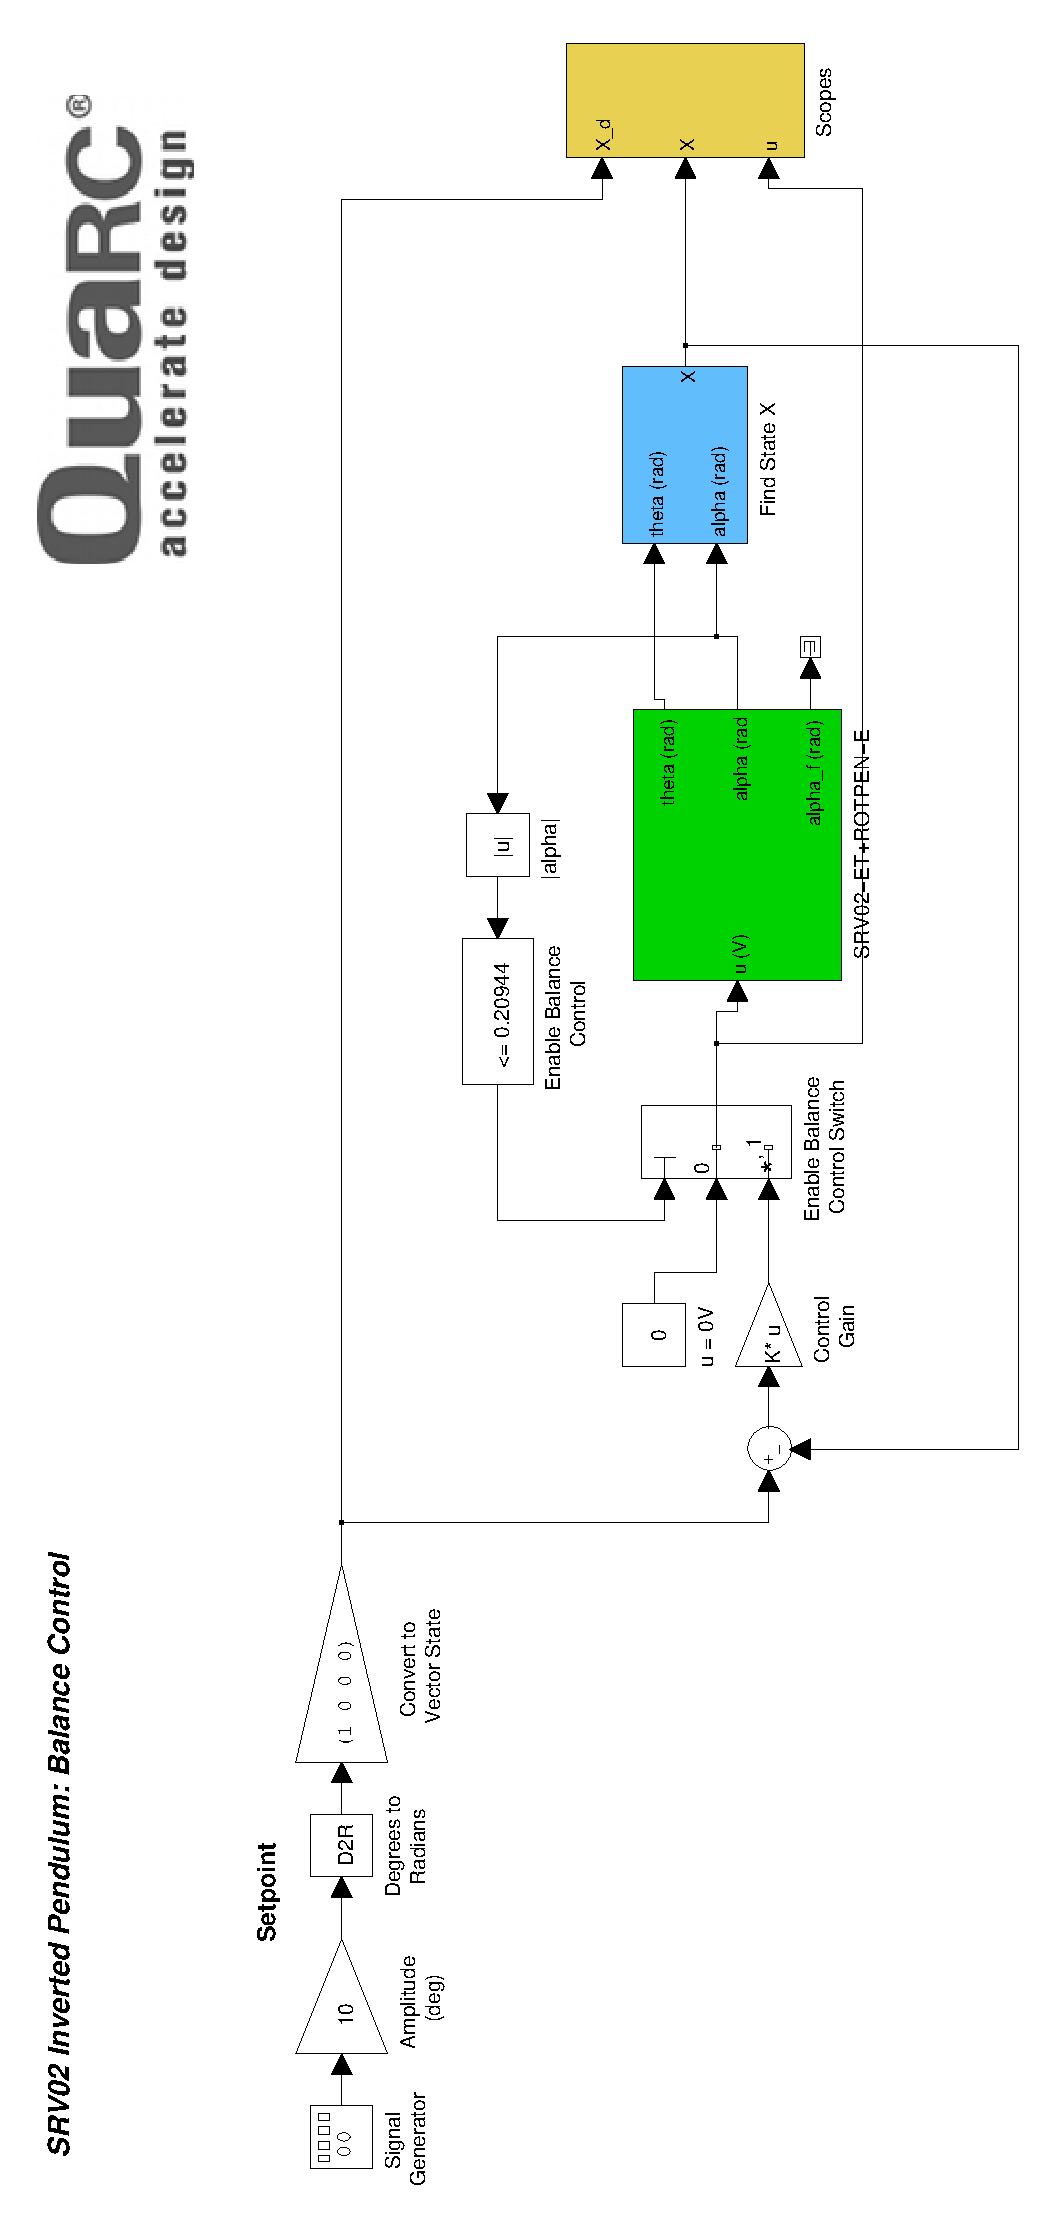
\includegraphics[width=0.5\linewidth,angle=-90]{eps/lab_3/balance_controller.eps}
    \caption{A Simulink model which interacts with the physical rotary pendulum system and uses state feedback in a small domain about the unstable equilibrium (i.e., inverted pendulum orientation) to balance the inverted pendulum.~\cite{Q-Flex-Beam}}
    \label{lab3_simulink_balance}
\end{figure}
\newpage
\begin{enumerate}[Questions]
    \item[Q5:] Record the results of the balancing experiment and plot your data. On one plot, compare the square wave input for the rotor base and the measured rotor base angle, $\theta$. On another plot, include the pendulum angle data, $\alpha$. Does your feedback controller manage to balance the inverted pendulum while tracking the square wave trajectory? What happens if you keep increasing the square wave amplitude, and why does this happen? What happens when you change the poles of the closed-loop system to be more negative in the left half-plane of $\mathbb{C}$ (i.e., designing the feedback gain, $K$, such that the closed-loop poles are much more negative)? For balancing the inverted pendulum, discuss the \emph{trade-offs between designing} the control system such that the poles of the closed-loop system are close to the origin or far in the left half-plane.\\
          \drew{Answer: Yes, it should be able to balance the inverted pendulum while tracking the square wave with amplitude of 10. If the amplitude is increased, then the pendulum angle may exceed the domain of validity of the linearization, and the feedback controller may not be able to balance the inverted pendulum.  Instructors should note that students' answers will vary, as the tension in the slip-gear will change the input required to balance the pendulum. When changing the poles of the closed-loop system by changing $F$, you change the rate of stabilization and the overshoot/undershoot of the stabilization. If one were to place these poles far in the left half-plane, then stabilization would be very immediate, but this immediate response comes at the cost of a large overshoot. In the case of the inverted pendulum, where the linearized system is only valid in a small neighbourhood about the inverted orientation, a large overshoot may be detrimental. Conversely, a very slow stabilization may allow the pendulum to fall outside the linearization's domain of validity, which also causes negative effects. Hence one must design and tune the feedback gain, $K$, for this application such that balancing stabilization is achieved quickly enough without a large overshoot. Here are the plots:
              \begin{figure}[htb!]
                  \centering
                  \subfigure{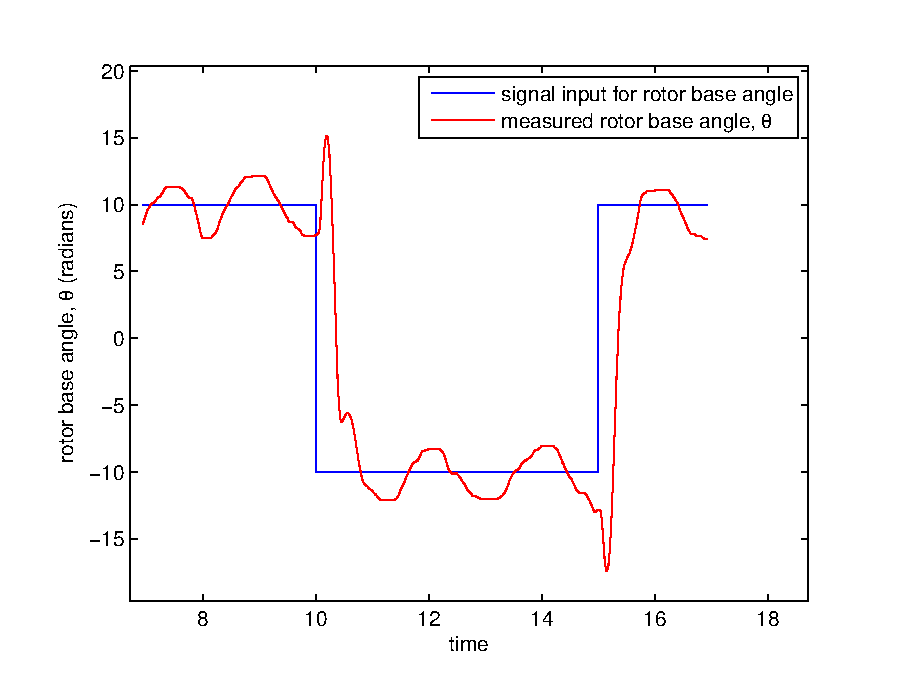
\includegraphics[width=0.4\linewidth]{eps/lab_3/full_feedback_balance_thetas.eps}} \quad
                  \subfigure{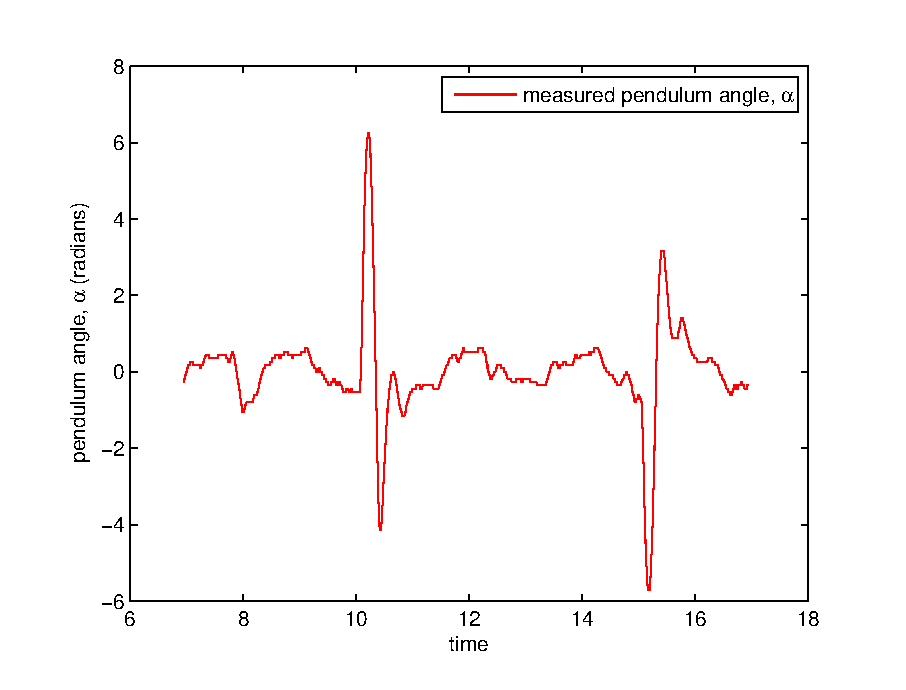
\includegraphics[width=0.4\linewidth]{eps/lab_3/full_feedback_balance_alpha.eps}}
                  \caption{(a) A plot of the desired and measured rotor base angle trajectories for the closed-loop feedback controller system while balancing the pendulum in the inverted orientation and while the rotor base tracks a square wave trajectory with amplitude 10, and; (b) a plot of the measured pendulum angle while the physical system tracks this square wave trajectory.}
                  \label{fig:lab3_state_feedback_response}
              \end{figure}
          }
\end{enumerate}

\subsection{Linear Observer}\label{subsection:lab3_observer}
Recall our linear time-invariant system dynamics
\[\mathbf{\dot{x}}(t)=A\mathbf{x}(t)+Bu(t) \quad \quad \quad \mathbf{y}(t)=C\mathbf{x}(t)\]
and consider the case where the encoder that reads the pendulum angle is damaged, i.e.,
\[C = \left[\begin{array}{c c c c}
            1 & 0 & 0 & 0 \\
            0 & 0 & 0 & 0
        \end{array}\right]\]
In this case, you do not have access to one of the system's internal states, $\alpha$. However, you may be able to determine the unknown state by using the system's input and output data. To do this, you will construct a linear dynamical system that produces an estimate of the physical system's state, also known as a \emph{linear state observer}.

\noindent \emph{Let us review some theory from class:}

Let us denote the state estimate by $\hat{\mathbf{x}}(t)$. David G. Luenberger proposed the following linear state observer~\cite{david1971introduction}:
\begin{equation}\label{lab3_equ:luenberger}
    \mathbf{\dot{\tilde{x}}}(t)=A\hat{\mathbf{x}}(t)+Bu(t)+L(\mathbf{y}(t)-C\hat{\mathbf{x}}(t)),
\end{equation}
where $L$ is the observer gain. Note that the input and measured output data are both used in~\eqref{lab3_equ:luenberger}. The observer in~\eqref{lab3_equ:luenberger} is composed of two parts: the first part, $A\hat{\mathbf{x}}(t)+Bu(t)$, is the rate of change of $\hat{\mathbf{x}}(t)$ as computed by the physical system's state-space model; the second part, $L(\mathbf{y}(t)-C\hat{\mathbf{x}}(t))$, is the difference between the observed output and the estimated output, scaled by the observer gain. Notice that without the second term, ~\eqref{lab3_equ:luenberger} becomes familiar:
\begin{equation}\label{lab3_equ:luenberger_simple}
    \mathbf{\dot{\hat{x}}}(t)=A\hat{\mathbf{x}}(t)+Bu(t).
\end{equation}
Let us denote the estimation error by $\tilde{\mathbf{x}}(t)$ and define it by $\tilde{\mathbf{x}}(t) = \mathbf{x}(t)-\hat{\mathbf{x}}(t)$. If one were to study the estimation error of the simplified observer~\eqref{lab3_equ:luenberger_simple}, then they would conclude that $\tilde{\mathbf{x}}(t)$ would go to zero when $\text{spec}(A) \subset \mathbb{C}^-$, as the error dynamic for~\eqref{lab3_equ:luenberger_simple} is
\begin{align*}
    \mathbf{\dot{\tilde{x}}}(t) & = A \left(\mathbf{x}(t)-\hat{\mathbf{x}}(t)\right)+Bu(t) - Bu(t) \\
                                & = A\tilde{\mathbf{x}}(t).
\end{align*}
That is, when matrix $A$ has all of its eigenvalues in the left half-plane, then the state estimate would converge to the actual state. But this convergence depends on the physical system's dynamics (thus the convergence rate can be quite slow, depending on the system) and the spectral constraints on $A$ are very restrictive. In contrast, the error dynamic for the Luenberger observer in~\eqref{lab3_equ:luenberger} is
\begin{equation}\label{lab3_equ:luenberger_error}
    \mathbf{\dot{\tilde{x}}}(t) = (A-LC) \tilde{\mathbf{x}}(t).
\end{equation}
Thus one can design an observer gain $L$ such that $\text{spec}(A-LC) \subset \mathbb{C}^-$ (i.e., an \emph{asymptotically stable observer}) and one can tune $L$ such that $\hat{\mathbf{x}}(t)$ converges to $\mathbf{x}(t)$ fast enough for the desired application. An important question to ask is, ``when does such an observer exist"? In class, you proved that one can build an observer with these properties when $(C,A)$ is \emph{detectable}.

\noindent \emph{Back to your lab:}

\textbf{Throughout this section, we'll be studying the rotary pendulum linearized about its stable equilibrium (i.e., the system from Lab 2). You will need your MATLAB files from Lab 2.}
\begin{enumerate}[Question]
    \item[Q6:] From your previous assessment on the controllablility \& observability of the rotary pendulum system when its pendulum encoder is damaged (Lab 2), can you hope to observe the unknown state $\alpha$ by designing and building an appropriate state observer? What does system detectability mean?\\
          \drew{Answer: Yes; since the system is observable when
              \[C = \left[\begin{array}{c c c c}
                          1 & 0 & 0 & 0 \\
                          0 & 0 & 0 & 0
                      \end{array}\right],\]
              it is also detectable, as detectability is a weaker notion of observability. System detectability implies that all of the system's unobservable states are asymptotically stable, but there are no unobservable states for this system.
          }
\end{enumerate}
One way to \emph{design an observer is by eigenvalue assignment}: the Luenberger observer error, $\tilde{\mathbf{x}}(t)$, governed by the differential equation~\eqref{lab3_equ:luenberger_error}, has a characteristic polynomial chosen by the designer. That is, the observer designer chooses $L$ such that the eigenvalues of $(A-LC)$ are at desired locations $p_1, p_2, \dots, p_n$. This design method has some benefits over other methods, mainly:
\begin{enumerate}
    \item theoretically, the observer error can decrease faster if the eigenvalues of $(A-LC)$ are more negative (however, there is a trade-off which you will explore), and;
    \item if the observed states are being used for state feedback, then the least negative eigenvalue of $(A-LC)$ should be more negative than the eigenvalues of the state feedback system $A-BK$. Loosely speaking, this dictates that the observer dynamics will converge to the unobserved states \emph{faster} than the system dynamics will change these states.
\end{enumerate}
One may notice a similarity between finding a feedback gain $K$ such that $A-BK$ has eigenvalues in $\mathbb{C}^-$ and finding an observer gain $L$ such that $A-LC$ also has eigenvalues in $\mathbb{C}^-$. Recall that the eigenvalues of a matrix and its transpose are the same. The problem of observer design is in fact the \emph{dual} of the state feedback problem, with the following equivalences~\cite{astrom2010feedback}:
\begin{align*}
    (A-LC)^T                      & = A^T - C^T L^T                                  \\
                                  & \leftrightarrow A - BK                           \\
    \\
    A \leftrightarrow A^T \quad B & \leftrightarrow C^T \quad K \leftrightarrow L^T.
\end{align*}

In \hyperref[subsection:lab3_feedback]{Section~\ref{subsection:lab3_feedback}}, you solved for $K$ by using the canonical controllable form and a similarity transformation. In MATLAB, there's a shortcut to solving for $K$ which uses the \emph{place} command. To solve for the feedback gain with desired poles at $\{-2.8 + 2.86i, \; -2.8 - 2.86i, \; -30, \; -40\}$, you can do the following in MATLAB:
\[
    p = [-2.8 + 2.86i \quad -2.8 - 2.86i \quad -30 \quad -40];
\]
\[
    K = place(A,B,p);
\]
\begin{enumerate}[Question]
    \item[Q7:] In MATLAB, how could you use the \emph{place} command to design observer gain $L$ such that $A-LC$ has its poles at $p =\{p_1, \; p_2, \; p_3, \; p_4\}$? \textbf{Hint:} duality.\\
          \drew{Answer: Using the duality of the observer and feedback design problems, and the equivalences stated above, you could use the MATLAB command
              \[
                  L = place(A',C',p)';
              \]
              to complete the task.}
\end{enumerate}

\subsubsection{Designing \& Validating an Observer}\label{sub subsection:lab3_observer_design}
You will now design an observer for the linearized rotary pendulum system, linearized about the \emph{stable equilibrium}. For this section of the lab, you'll need the state-space matrices $A$, $B$, $C$ and $D$ that you calculated in \hyperref[lab2:linearization_validity]{Section~\ref{lab2:linearization_validity}} of Lab 2. You should alter your $C$ matrix so that only the rotor base angle, $\theta$, is outputted, as you are studying the case where the encoder reading the pendulum angle is damaged. Figure~\ref{figure:lab3_luenberger_block} shows a Simulink block diagram for a Luenberger observer; you will integrate this observer subsystem into a Simulink model to compare the actual and estimated states.
\begin{figure}[htb!]
    \centering
    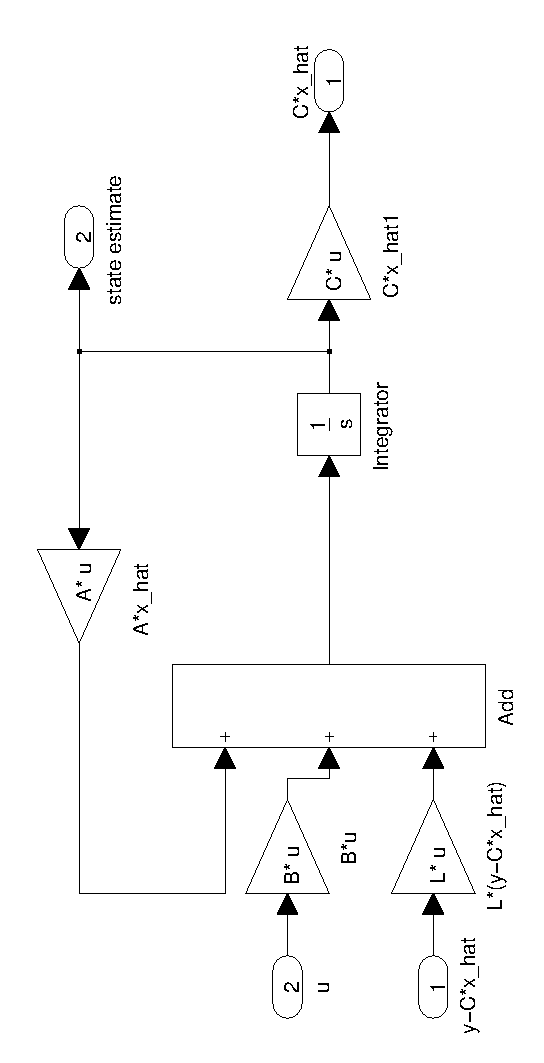
\includegraphics[width=0.4\linewidth,angle=-90]{eps/lab_3/luenberger_subsystem}
    \caption{A Simulink block diagram of a Luenberger observer. This is a subsystem block that can be incorporated into a Simulink model, along with a state-space subsystem block, to compare the estimated and the actual states.}
    \label{figure:lab3_luenberger_block}
\end{figure}
\newpage
Open the Simulink model \textbf{luenberger\_openloop\_model.mdl}. Note that the regular State-Space block is not used to model the linearized rotary pendulum system; in place, we've created a subsystem block that does this, and it is shown in Figure~\ref{figure:lab3_statespace_block} along with the Luenberger observer subsystem block.
%The state-space subsystem that we've created allows you to access all of the system's states at a given time and output them into the MATLAB workspace, whereas the State-Space block only outputs $y=Cx$. Thus, you must use this subsystem block for the state-space dynamics so that you can compare the actual states and the state estimates produced by your observer.
\begin{figure}[htb!]
    \centering
    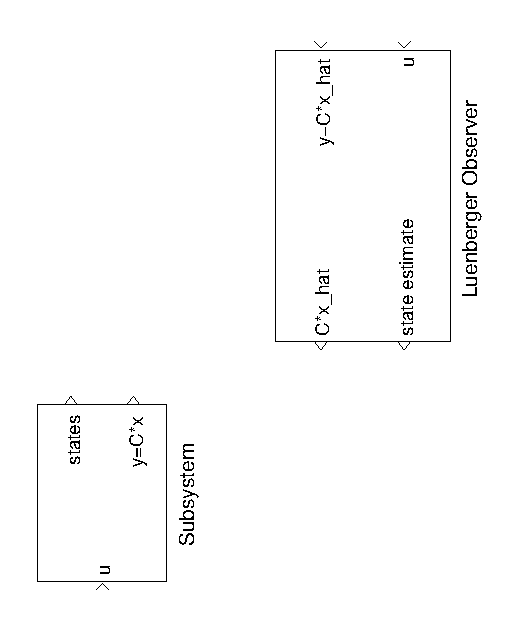
\includegraphics[width=0.4\textwidth,angle=-90]{eps/lab_3/luenberger_openloop_student}
    \caption{A Simulink block diagram of a state-space subsystem \& Luenberger observer subsystem. The state-space subsystem block allows one to output the usual $y=Cx$ output as well as outputting all of the states at each time, making it useful for state estimate validations.}
    \label{figure:lab3_statespace_block}
\end{figure}

Connect these two Simulink subsystem blocks so that the observer can estimate the states of the linearized state-space model of the rotary pendulum. Now, add a Signal Generator block, a Sum or Add block, and a DegreesToRadians block to the Simulink model and use a sine signal with amplitude 10 as your input (transforming your input to radians using the DegreesToRadians block). In the state-space subsystem, set the initial conditions (found in the integrator block) of your states to zero (in MATLAB, this is done with the vector $[0;0;0;0]$), and set the initial conditions of your observer subsystem to non-zero values between $[-10,10]$. Make sure to output your states and your state estimates to your workspace using To Workspace blocks.

\begin{enumerate}
    \item[Q8:] Run various tests using this model while changing the observer's poles in $\mathbb{C}^-$. First, \emph{design and tune your observer} so that the state estimates converges to the actual states very quickly; second, try to achieve state estimates that don't deviate from the actual states too much. \emph{What metrics you would use to evaluate} your observer (and the resulting observer gain design) were it to be used for: state feedback to balance the inverted pendulum, and; monitoring an industrial process where large spikes cause the industrial plant to shut down.\\
          \drew{Answer: Tuning the observer gain such that the state estimates converge very quickly to the actual states (i.e., the observer poles are far in the left half-plane) comes at the cost of a very large overshoot. Thus, it is important to design the observer gain so that this tradeoff be exploited for a given application. For the inverted pendulum application, since the domain of validity for the linearized system is a small neighbourhood about the inverted orientation, a large overshoot in the pendulum angle state estimation would make the ensuing feedback response overcompensate unnecessarily. Conversely, a slow state estimate convergence can make the ensuing feedback response much to slow to keep the inverted pendulum in the linearized system's domain of validity. This is why this physical stabilization problem is not considered - it is much too finicky to work, and may require techniques other than gain tuning to make it work properly. Some metrics may include overshoot, settling time, energy used in state feedback, etc. For the monitoring application, one would choose to design the observer poles close to the origin since large state estimate overshoots would cost the industrial plant much lost time. The main metric here is overshoot, among other engineering metrics.}
\end{enumerate}
\subsubsection{Testing your Observer on the Physical System}\label{sub subsection:lab3_observer_test}
In this section, you will verify that the observer you built for the state-space model works for the physical system. This will help you identify the benefits and drawbacks of different observer tunings for gain $L$. Open the Simulink model \textbf{luenberger\_openloop\_quanser.mdl}. When accessing the rotary pendulum subsystem block, one will notice that the Luenberger observer is nested into this subsystem, as shown in Figure~\ref{figure:lab3_luenberger_openloop_quanser}. This subsystem outputs the measured and the estimated pendulum angle, so that these angles can be compared directly.
\begin{figure}[htb!]
    \centering
    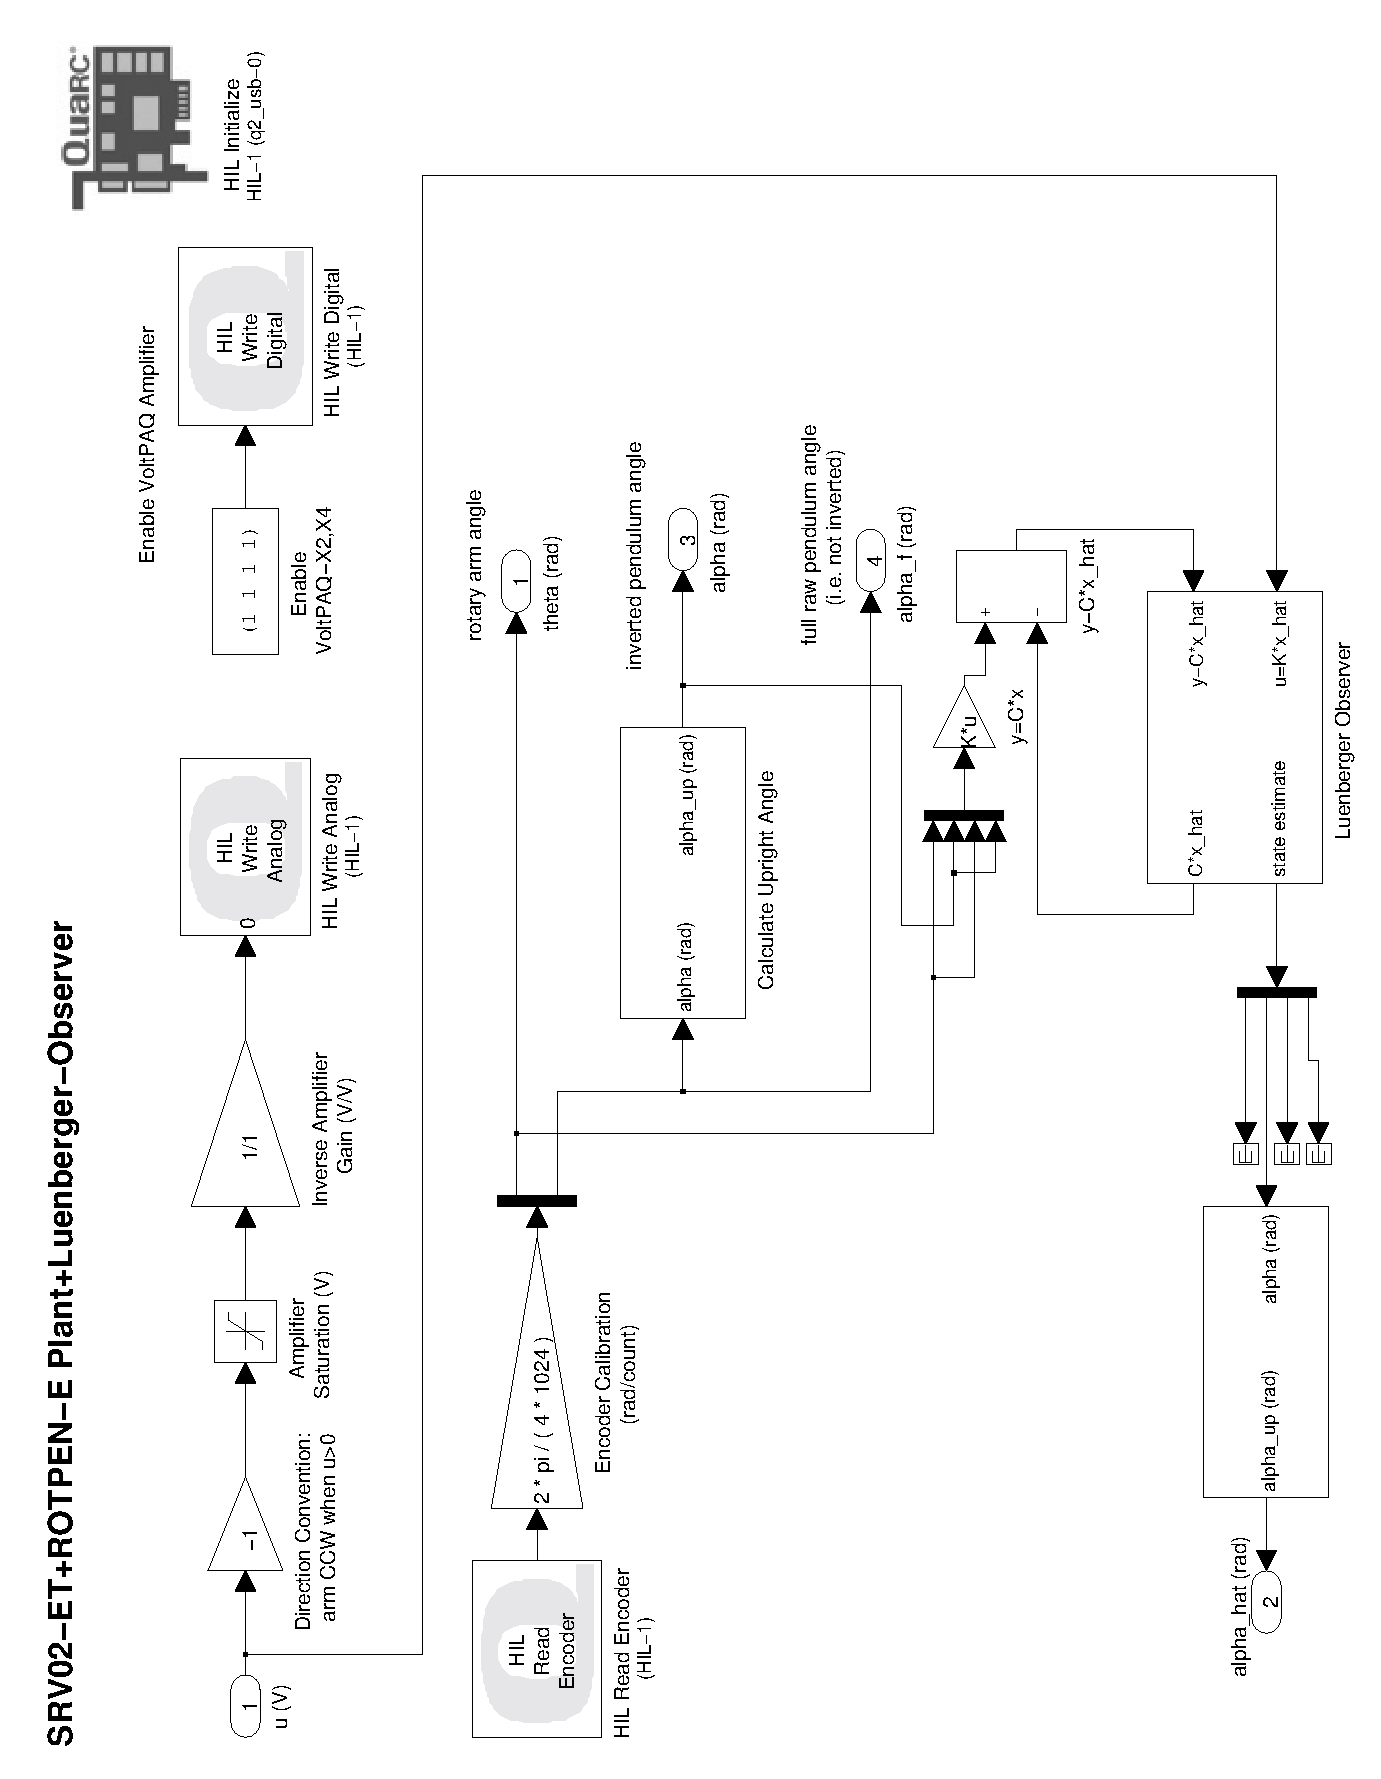
\includegraphics[width=0.6\linewidth,angle=-90]{eps/lab_3/luenberger_openloop_quanser}
    \caption{A Simulink model of a Luenberger observer estimating \& outputting the pendulum angle, $\hat{\alpha}$, for the physical rotary pendulum system. Note that in the Luenberger observer, measured states $\dot{\theta}$ and $\dot{\alpha}$ are non needed, as they are scaled by $C$.}
    \label{figure:lab3_luenberger_openloop_quanser}
\end{figure}
\newpage
\begin{enumerate}
    \item[Q9:] Build \& run \textbf{luenberger\_openloop\_quanser.mdl}, with a sine wave input with amplitude of 1 and frequency of 5 $rad/s$. First, use [0,\; 0,\; 0,\; 0] as the initial conditions for the observer. Plot the measured and the estimated pendulum angle, $\alpha$ and $\hat{\alpha}$, with respect to time when your observer has poles $\{-5,\; -6,\; -7,\; -8\}$. Repeat the experiment for observer poles $\{-15,\; -16,\; -17,\; -18\}$, and then for observer poles $\{-45,\; -46,\; -47,\; -48\}$ (creating the same plots for each experiment). Repeat these for the case where the initial conditions of the observer are not identically zero. From these plots, what can you conclude about the relationship between the accuracy of the state estimates produced by your Luenberger observer and \emph{the design and tuning} of the observer gain, $L$? Give two different real-life applications where state observers could be used, and what \emph{metrics} would you develop to evaluate these observers in the setting of their respective applications (specifically look at the relationship between observer behaviour and pole placement via observer gain, $L$).\\
          \drew{Answer: one will note that the observer error after a crest of the sine wave input cannot be completely eliminated for these three observer gains, as some observer error is present in all three plots. The penalty for having very negative observer poles is apparent: while the observer dynamic is very fast, it quickly acts on a control input and then reacts to reduce the estimate output error term ($L(y-C\hat{x}(t)$), and does so frequently. For observer poles at $\{-15,\; -16,\; -17,\; -18\}$, the observer gives a most accurate estimate, but the observer is still a bit too sensitive to control inputs. Due to the constant change in the input signal, the observer estimate error never has time to converge to zero. I will leave the engineering-based responses to be answered by the current TA.
              \begin{figure}[htb!]
                  \centering
                  \subfigure{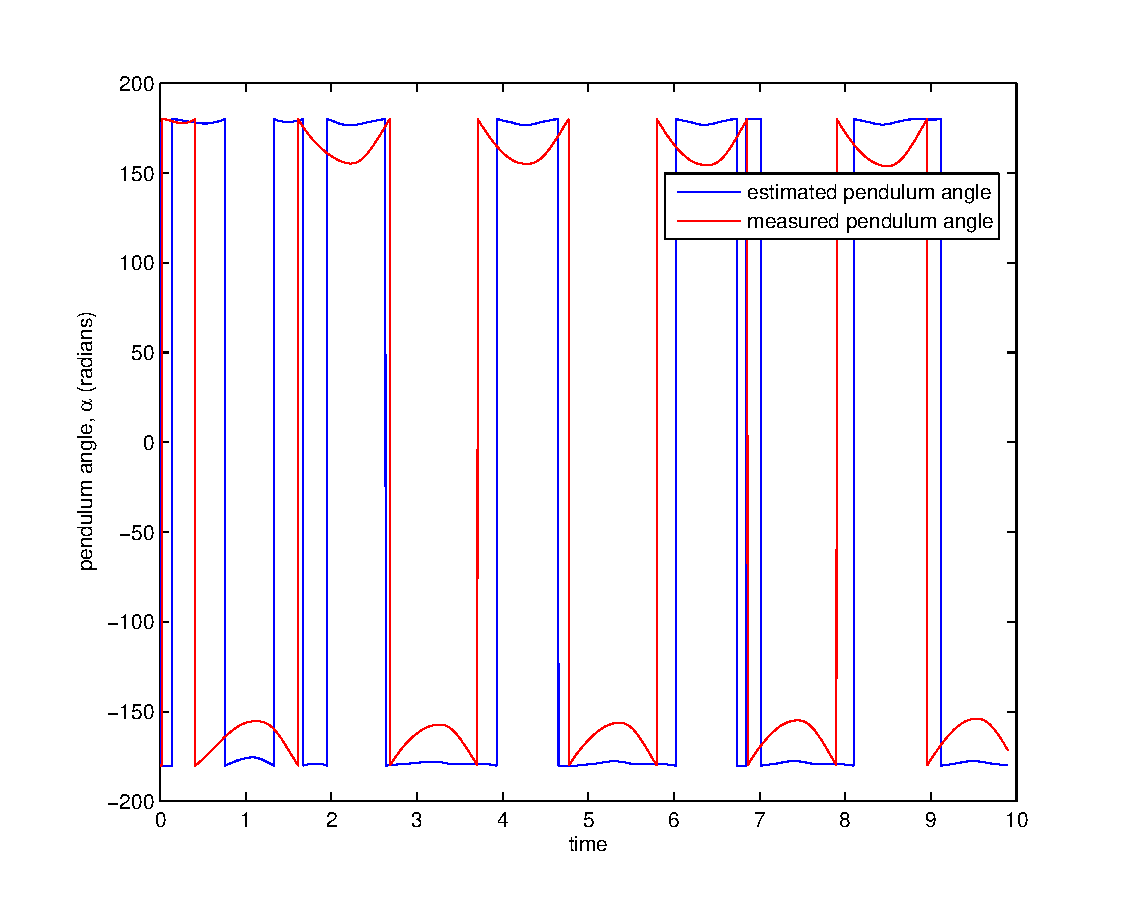
\includegraphics[width=0.4\linewidth]{eps/lab_3/luenberger_openloop_quanser_exp1}}
                  \subfigure{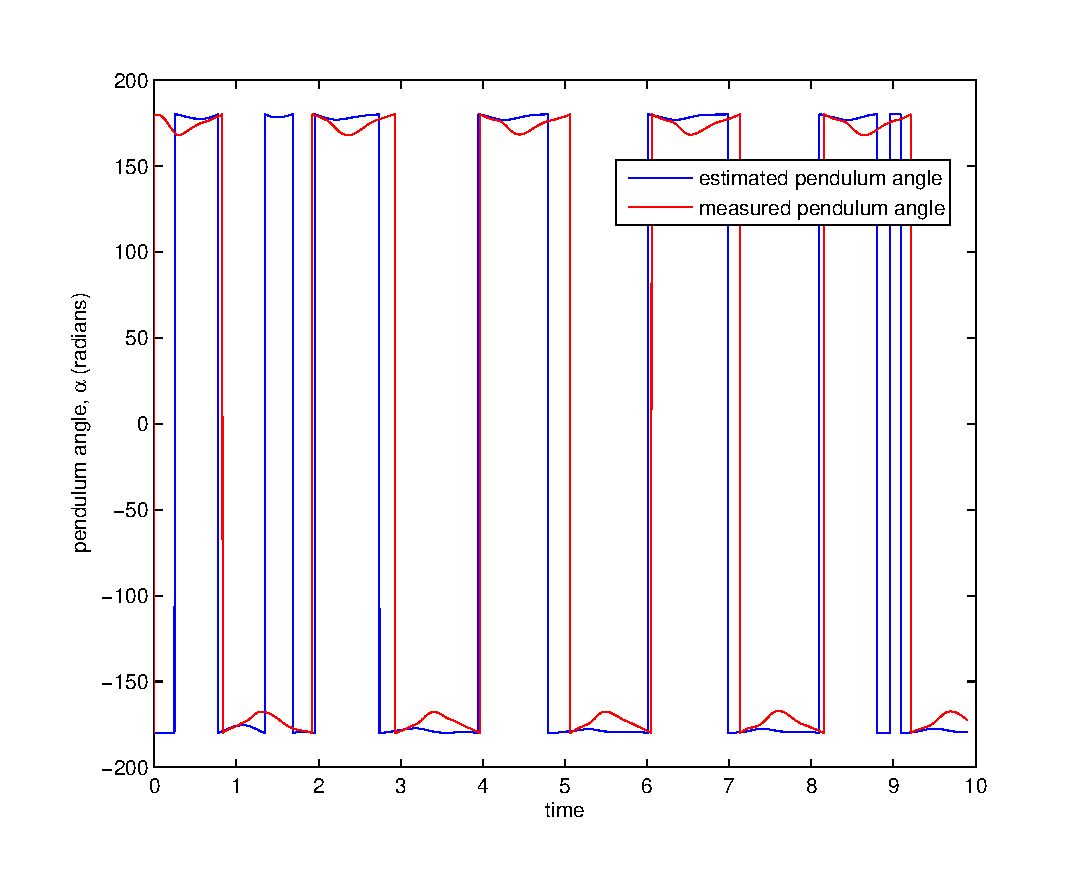
\includegraphics[width=0.4\linewidth]{eps/lab_3/luenberger_openloop_quanser_exp2}}
                  \subfigure{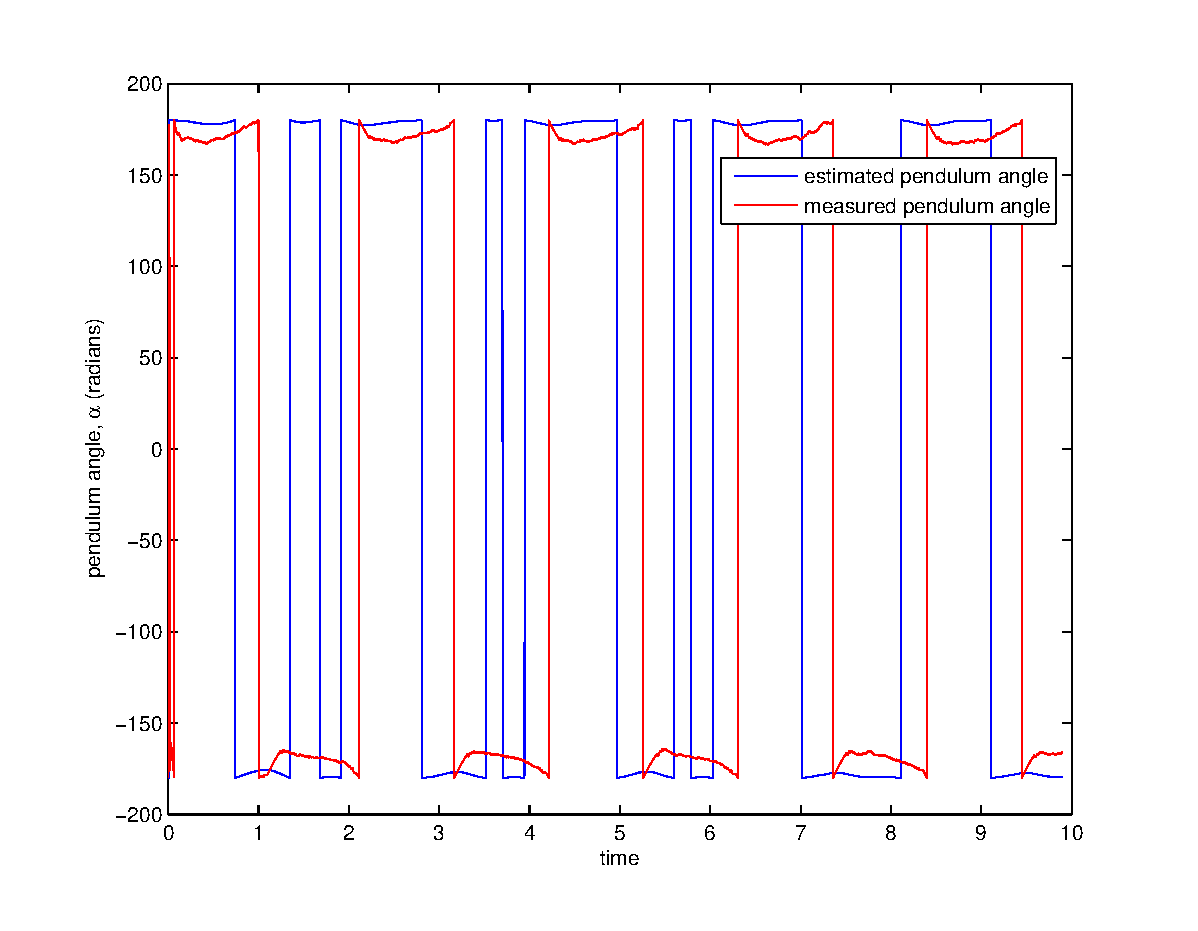
\includegraphics[width=0.4\linewidth]{eps/lab_3/luenberger_openloop_quanser_exp3}}
                  \caption{Plots comparing the measured and estimated pendulum angle response to a sine wave input of amplitude of 0.5 and frequency of 3 $rad/s$ for observer gains a) $L = \{-5,\; -6,\; -7,\; -8\}$, b) $L = \{-15,\; -16,\; -17,\; -18\}$ and c) $L = \{-45,\; -46,\; -47,\; -48\}$.}
              \end{figure}
          }
\end{enumerate}
\newpage
%\subsubsection{Balance Feedback Control using State Estimate}\label{subsubsection:lab3_observer_feedback}
%Now, you'll verify whether you can use your state estimate of $\alpha$, denoted $\hat{\mathbf{\alpha}}$, as well as your measured state, $\theta$, to construct a feedback loop which will make the linearized rotary pendulum system, linearized about the \emph{unstable equilibrium} (i.e., inverted orientation), asymptotically stable.
%
%\begin{enumerate}[Questions]
%\item[Q9:] Is the linearized rotary pendulum system, linearized about $\alpha = 0$ (unstable equilibrium), \emph{detectable}, and why? Is it \emph{stabilizable}, and why? What can be concluded about the viability of using $\hat{\mathbf{\alpha}}$ and $\theta$ as feedback to balance the rotary pendulum in the inverted orientation?\\
%\drew{Answer: Recall that a system is said to be \emph{detectable} if and only if all of its unstable modes are observable (i.e., if all of its unobservable modes are asymptotically stable). Another way to see this is the following: a system is said to be detectable if $\mathbf{y}(t) \rightarrow 0$ implies that $\mathbf{x}(t) \rightarrow 0$. This is untrue for the state $\alpha$ linearized around the unstable equilibrium, thus a Luenberger observer does not exist for our system.}
%
%\drew{A system is said to be \emph{stabilizable} if and only if all of its unstable modes are controllable (i.e., if all of its uncontrollable modes are stable). Note that this definition necessarily implies that if a system is controllable, it is stabilizable (no uncontrollable unstable modes). As you've already shown that this system is controllable, then it follows that it is stabilizable.}
%
%\drew{An equivalent definition for stabilizability and detectability is as follows:
%\begin{itemize}\label{lab3:stabilize_detect_defs}
%\item given a pair $(A,B)$, we say that $(A,B)$ is \textbf{stabilizable} if there exists $K$ such that $A-BK$ is Hurwitz, and;
%\item given a pair $(C,A)$, we say that $(C,A)$ is \textbf{detectable} if there exists $L$ such that $A-LC$ is Hurwitz.
%\end{itemize}}
%
%\drew{Recall a result from class that one can use state estimate feedback to place the poles of the closed-loop system at $\mathcal{X}_{(A-LC)} \cdot \mathcal{X}_{(A-BK)}$. Thus, it follows from the alternate definitions of stabilizability and detectability that one can only place the closed-loop poles of the linearized rotary pendulum system in $\mathbb{C}^-$ if it is \textbf{both stabilizable and detectable}, which it is not.}
%\end{enumerate}

%Open the Simulink model \textbf{luenberger\_closedloop.mdl}, shown in Figure~\ref{figure:lab3_luenberger_closedloop}. You'll notice that in place of using the measured pendulum angle as was done in Section~\ref{subsection:lab3_feedback}, the feedback loop uses the estimated pendulum angle. As briefly discussed earlier, when using the state estimate in a feedback loop, one must be careful to choose the eigenvalues of $A-LC$ carefully so that the state estimate dynamics are \emph{faster} than the system's dynamics. A starting point to choose the poles of the observer is to place them five times more negative than the dominating poles of $A-BK$. Recall that the dominating poles are usually those that are closest to the imaginary axis, as they are \emph{slowest} in the sense that they give rise to the longest lasting terms in the transient response of the system.
%\begin{figure}[htb!]\label{figure:lab3_luenberger_closedloop}
%\centering
%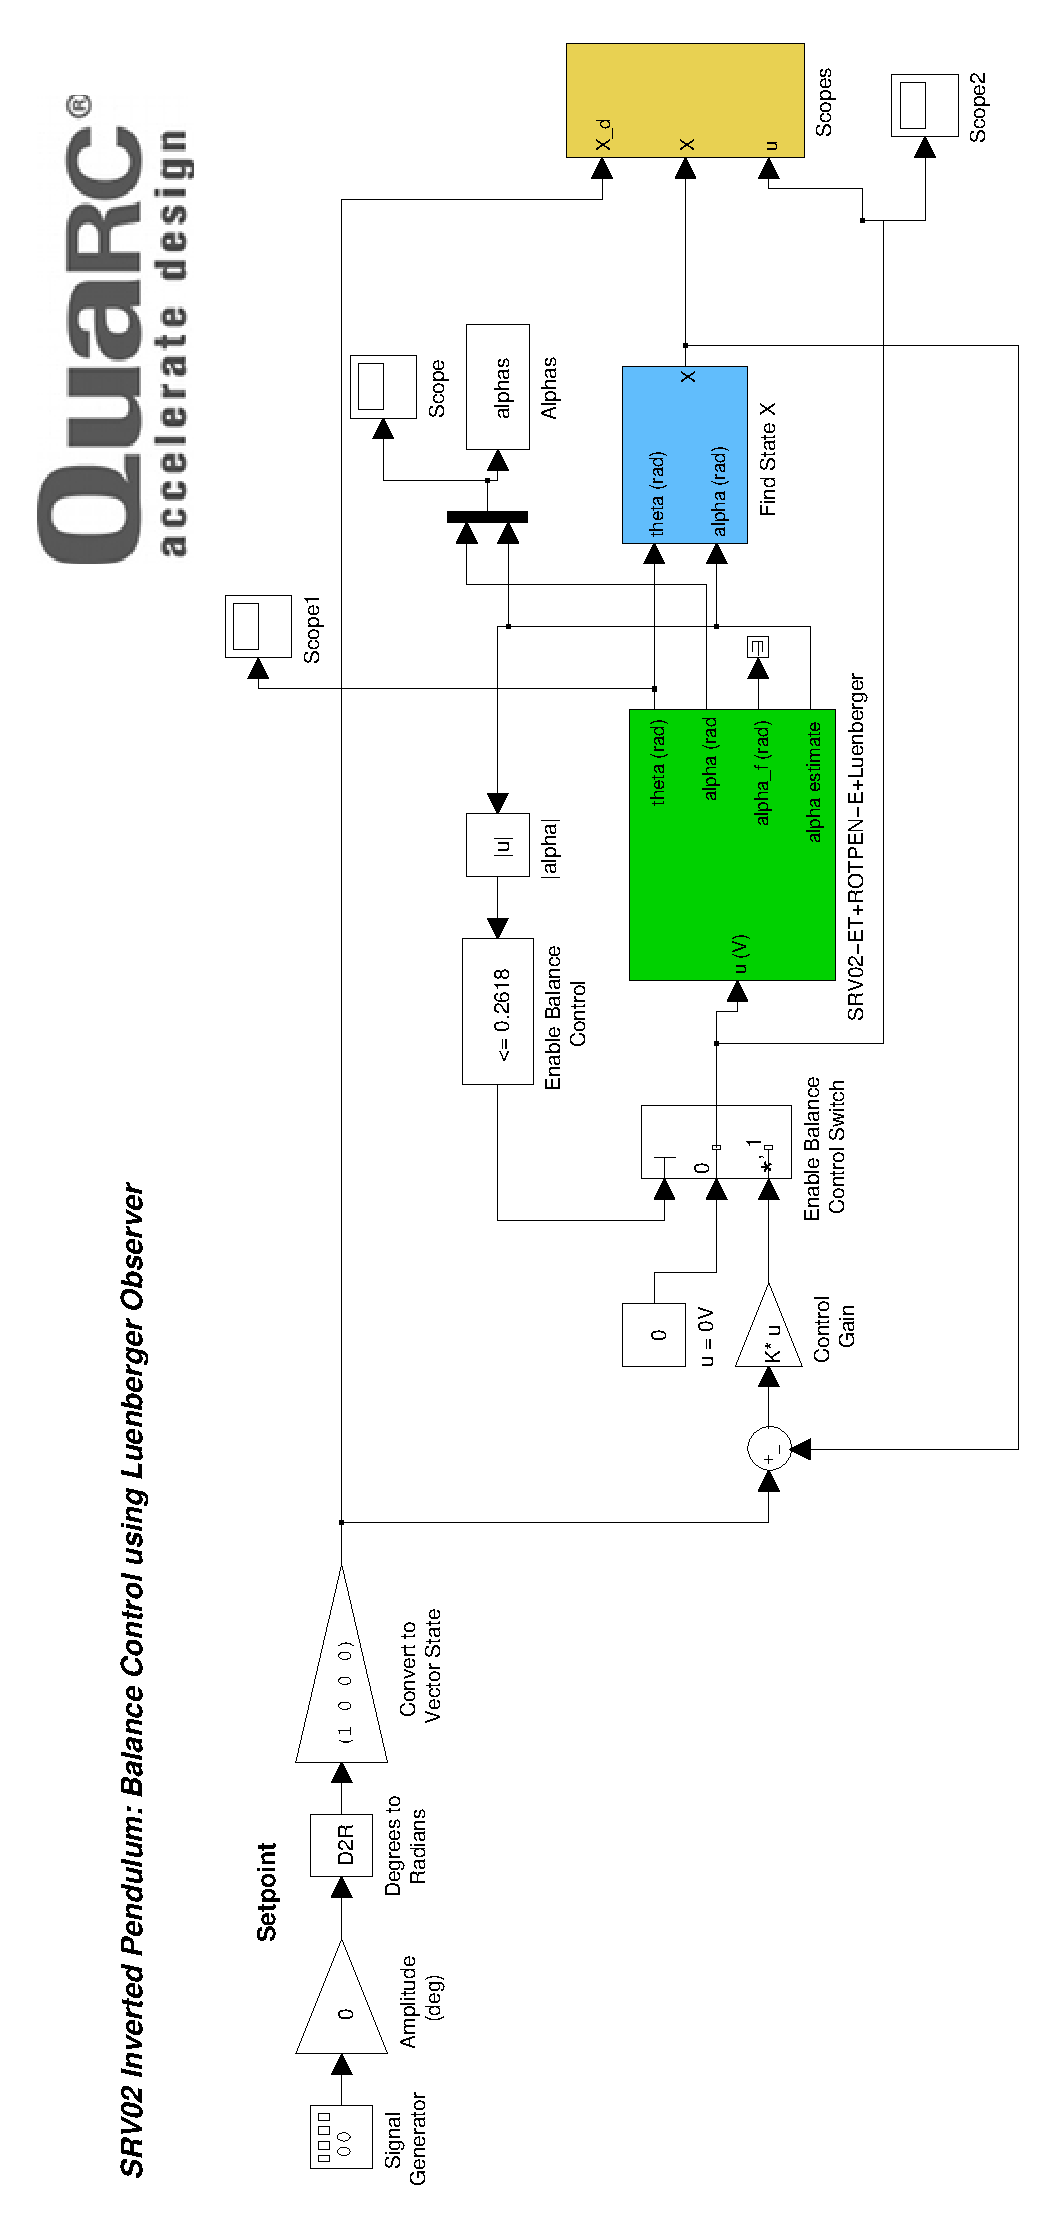
\includegraphics[width=0.5\textwidth,angle=-90]{eps/lab_3/balance_controller_luenberger}
%\caption{A closed-loop feedback system for the rotary pendulum using partial state feedback and state estimate feedback.}
%\end{figure}
%
%The nature of this experiment is to tune the observer gain, $L$, so that the state estimates are accurate enough to achieve balance control. To tune $L$, you should compare the measured pendulum angle and the estimated pendulum angle using a Scope block (to compare in real-time). After downloading the Simulink model to the target and pressing Run, you can lift the pendulum slightly, observe the error in the pendulum angle estimate via the Scope block, and tune the observer gain appropriately. You should start by setting the poles of $A-LC$ at five times more negative than the dominating pole among $\{-2.8 + 2.86i, \; -2.8 - 2.86i, \; -30, \; -40\}$. \textbf{Note:} you cannot have algebraic multiplicity greater than one when using the \emph{place} command, so you'll have to separate these poles by some numbers that you choose).
%
%Once your observer gain is properly tuned, you can lift up the pendulum to the inverted orientation and see if your control system can achieve balancing the pendulum.
%
%\begin{enumerate}[Questions]
%\item[Q8:] First, plot your measured and your estimated pendulum angle with respect to time. Next, plot your control input with respect to time. Did your control system balance the inverted pendulum using partial state feedback and state estimate feedback? Where did you place the poles of your observer gain to achieve this balance control?\\
%\drew{Answer: Yes, the control system managed to balance the inverted pendulum by using an observer gain of $L = \{-90,\; -92,\; -92.5,\; -93  \}$:
%\begin{figure}[htb!]
%\centering
%\subfigure{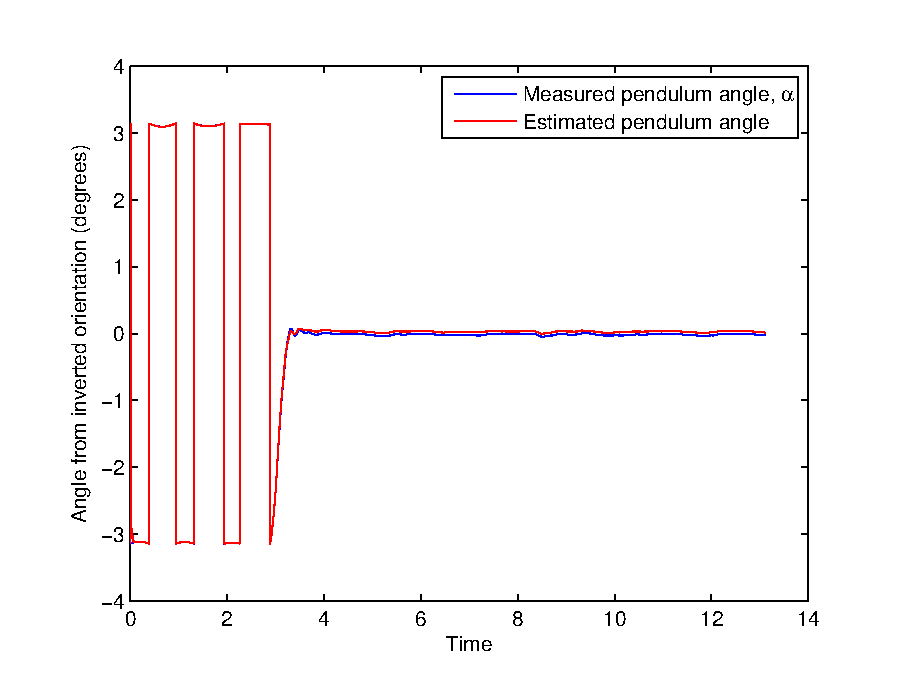
\includegraphics[width=0.5\linewidth]{eps/lab_3/luenberger_closed_loop_alphas}}
%\subfigure{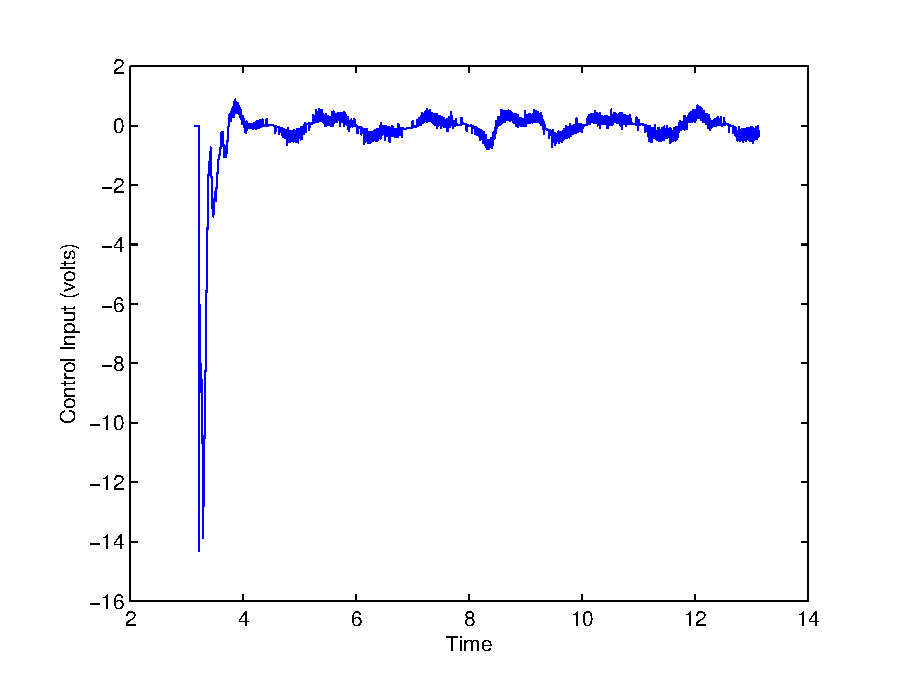
\includegraphics[width=0.5\linewidth]{eps/lab_3/luenberger_closed_loop_input}}
%\caption{Plots of the estimated and measured pendulum angle, $\alpha$, and the control input. Note that the estimated and measured $\alpha$ agree very well, and one can observe that the control system does balance the inverted pendulum just past three seconds. The control input is constantly adjusting the rotor base to allow the pendulum to stay upright.}
%\end{figure}}
%\end{enumerate}

\subsection{Deliverables}
To recap the lab objectives, this is what you need to include in your lab report to obtain full marks:
\begin{enumerate}
    \item prelab question (i) through (vi), and;
    \item the answers to questions Q1, Q4, Q5, Q8 and Q9 (include plots where requested).
\end{enumerate}
\textbf{Note: Save your lab report and have an electronic copy on-hand in all future labs, as you will need some of the values obtained in this lab to build upon this physical system.}
%----------------------------------------------------------------------------------------
%	Lab 4
%----------------------------------------------------------------------------------------
\newpage
\section{Lab 4: LQR Optimization for Feedback Control and Observer Design for the Rotary Flexible Beam} \label{section:lab4}

\subsection{Introduction}\label{subsection:lab4_intro}

The purpose of this lab is to design and optimize a feedback controller for the rotary flexible beam system. One way of achieving this is to use a Linear Quadratic Regulator, which automates the process of finding a state feedback gain $K$ in a way that optimizes the system for certain design parameters. The prelab focuses on analyzing the stability of the open-loop rotary flexible beam system. In the lab, you will first design and optimize the closed-loop state feedback system by using the LQR technique to minimize the flexible beam's deflections while the rotor base tracks an input signal trajectory. The closed-loop system will have to adhere to set restrictions on settling time, percent overshoot and maximal flexible beam deflection. Next, you will observe the effects of using only partial state feedback on the system response to an input. Finally, you will attempt to minimize these system response effects by building an observer for the unobservable state and using the ensuing state estimate as feedback.
\begin{figure}[htb!]
    \centering
    \includegraphics[width=.6\linewidth]{eps/lab_1/quanser.eps}
    \caption{Qanser SRV02 with flexible beam module~\cite{Q-Flex-Beam}.}
    \label{fig:lab4_plant}
\end{figure}

\subsection{Prelab: Open-Loop Stability Analysis}\label{subsection:lab4_prelab}
Recall the 2-DOF state-space matrices that you found in \hyperref[subsubsection:lab1_modelvalidation]{Section~\ref{subsubsection:lab1_modelvalidation}} of Lab 1.

\begin{enumerate}
    \item What are the poles of the open-loop state-space representation of the rotary flexible beam system? What can you conclude about the stability of this open-loop system? Does this make sense from a physical point of view?\\
          \textbf{Hint:} When we talk about systems without any controls intervention, we are referring to \emph{internal} stability. For a quick review of internal stability, see your MTHE 332 course notes~\cite[p. 162]{AL:04}.\\
          \drew{Answer: The open-loop poles are $\{0,\; -8.13+22.47i,\; -8.13-22.47i,\; -24.21\}$, and both the algebraic and geometric multiplicities are equal, thus the system is internally stable.}
    \item Can we hope to use full state feedback to steer the rotary flexible beam system?\\
          \drew{Answer: To verify this, one must compute the controllability matrix of the system:
              \[
                  \mathcal{C}_{(A,B)} = \left[\begin{array}{c c c c}
                          0      & 61.77    & -2501.26  & 62750.59   \\
                          0      & -61.77   & 2501.26   & -41639.42  \\
                          61.77  & -2501.26 & 62750.59  & -980692.86 \\
                          -61.77 & 2501.26  & -41639.42 & 125861.00
                      \end{array}\right]
              \]
              The system's controllability matrix has full rank, and hence the system is controllable. Thus, we can hope to use full state feedback and pole placement techniques to control the system.}
    \item If the system is steerable, what \emph{metrics} would you develop to evaluate your state feedback controller against others for different \emph{engineering applications} (e.g., when the rotary pendulum is used to sort boxes on a conveyor belt in the warehouse of an online retailer; or when the rotary pendulum is mounted underwater for tidal wave energy production, and control input keeps it from becoming unstable)?\\
          \drew{Answer: I'll leave this to the imagination of the students/TA}
\end{enumerate}

\subsection{Designing Feedback using the Linear Quadratic Regulator}\label{subsection:lab4_lqr}
A fundamental problem in control theory is operating a control system at minimum cost. When concerned with linear differential equations (e.g., $\mathbf{\dot{x}}(t) = A\mathbf{x}(t) + Bu(t)$) and quadratic cost functions, then one is really concerned with the \emph{LQ problem}. In this lab, we will use a main result from this area of literature~\cite{kwakernaak1972linear} which is the solution to the linear quadratic regulator (LQR). The solution to the LQR will help you design a feedback controller which minimizes the deflections of the flexible beam while the rotor base tracks a square wave trajectory (within certain \emph{design constraints} on settling time and overshoot).

\noindent \emph{Let us review some theory from class:}

The LQ problem that we are dealing with is an infinite-horizon problem that studies the control system
\[
    \begin{cases}
        \dot{\mathbf{x}}(t) = A\mathbf{x}(t)+Bu(t), \quad \text{where} \; \mathbf{x}(0) = \mathbf{x}_0 \\
        \mathbf{y}(t) = C \mathbf{x}(t)
    \end{cases}
\]
subject to minimizing the cost function
\[
    \eta(u) = \int_0^{\infty} \mathbf{y}^T(t)\mathbf{y}(t) + u^T(t)u(t) \; dt = \int_0^\infty  \mathbf{x}^T(t) C^T C \mathbf{x}(t) + u^T(t)u(t) \; dt.
\]
You may think of the first part of the cost function, $ \int_0^{\infty} \mathbf{y}^T(t)\mathbf{y}(t) dt$, as the \emph{energy of the controlled output}, and the second part, $\int_0^{\infty} u^T(t)u(t) dt$, as the \emph{energy of the control input}.

Two \textbf{main results} from class follow this reformulation: the first is that if $(A,B,C)$ is a minimal realization, then there exists a positive definite symmetric solution $\Pi_{\infty} \in \mathcal{M}^{n \times n}(\mathbb{R})$ to the continuous algebraic Ricatti equation (CARE):
\[
    A^T \Pi_{\infty} + \Pi_{\infty} A - \Pi_{\infty} B B^T \Pi_{\infty} = -C^T C;
\]
the next main result is that with $(A,B,C)$ a minimal realization, the controller
\[
    u(t) = -B^T \Pi_{\infty} \mathbf{x}(t)
\]
solves the LQ problem.

\begin{enumerate}[Question]
    \item[Q1:] What does it mean to be a minimal realization? Is the state-space model of the rotary flexible beam system a minimal realization? Can one hope to use the LQR approach to optimize the feedback control inputs for the rotary flexible beam system?\\
          \drew{Answer: Given any transfer function, any state-space model that is both controllable and observable and has the same input-output behaviour as the transfer function is said to be a minimal realization. As was shown in Lab 1, the state-space model of the rotary flexible beam accurately describes the physical system; since the transfer function describes the input and output behaviour of the physical system, one can conclude that the state-space model has the same input-output behaviour as the transfer function. Furthermore, the observability matrix for the state-space model is
              \[
                  \mathcal{O}_{(C,A)} = \left[\begin{array}{c c c c}
                          1 & 0         & 0        & 0       \\
                          0 & 1         & 0        & 0       \\
                          0 & 0         & 1        & 0       \\
                          0 & 0         & 0        & 1       \\
                          0 & 623.77    & -40.49   & 0       \\
                          0 & -965.53   & 40.49    & 0       \\
                          0 & -25257.84 & 1639.61  & 623.77  \\
                          0 & 25257.84  & -1639.61 & -965.53
                      \end{array}\right]
              \]
              which has full rank (see prelab for computation of $\mathcal{C}_{(A,B)}$, which also has full rank). Thus, $(A,B,C)$ is a minimal realization, and one can use the main results for LQR theory to optimize the feedback control inputs for the physical system.
          }
\end{enumerate}

\noindent \emph{Back to your lab:}

There are a few differences in the theory that you've learned from class and the treatment we will apply here. First, we wish to minimize some of the system's outputs more than others, e.g., our focus is on minimizing the flexible beam deflections. With this focus, we present a more generalized form of the quadratic cost function:
\begin{equation}\label{lab4_cost_function}
    \eta(u) = \int_0^{\infty} \mathbf{x}^T(t) Q \mathbf{x}(t) + u^T(t)u(t) \; dt,
\end{equation}
where $Q$ is symmetric and $\mathbf{x}^T(t) Q \mathbf{x}(t) > 0$ for all $t$ (positive-definite). You will set the matrix $Q$ as a diagonal weighting matrix to assign different weights on the states within the cost function~\eqref{lab4_cost_function}. In turn, this will determine how the control input $u(t)$ will minimize the cost function $\eta(u)$, and thus the weightings of matrix $Q$ will have direct effects on the ensuing feedback gain, $K$. Hence, the LQR design process is really an iterative process: tune the diagonal weightings of $Q$, observe the effects, compare against the desired performance metrics, and repeat.

In the theory from class, one had to verify that $(A,B,C)$ was a minimal realization in order for $u(t)=-B^T \Pi_{\infty} \mathbf{x}(t)$ to solve the LQ problem. Using the generalized quadratic cost function in~\eqref{lab4_cost_function}, one must only verify that $(A,B)$ be stabilizable to ensure that this input solves the LQ problem. Can the LQR approach be used to optimize the feedback control inputs for the rotary flexible beam?\\
\drew{Answer: stabilizability follows from the fact that the system is controllable (see previous answer for $\mathcal{C}_{(A,B)}$ computation).}

Open the Simulink model \textbf{lqr\_model.mdl}, shown in Figure~\ref{lab4_lqr_simulink}. You may have to connect the physical system to the computer, as was done in \hyperref[sub subsection:lab1_setup]{Section~\ref{sub subsection:lab1_setup}} of Lab 1. Notice the presence of a high-gain observer, used to estimate the time derivatives of the signals $\theta$ and $\alpha$, as was discussed in \hyperref[subsection:lab3_feedback]{Section~\ref{subsection:lab3_feedback}} of Lab 3. In this lab, you will use these signal derivative estimates as feedback. Notice also that the output signal is subtracted from the input signal before being scaled by the feedback gain. Thus when the system's outputs match the system's inputs, a signal of all zeros will be input into the physical system; when the system inputs and outputs do not match, the feedback gain should be designed to drive the non-zero states to zero (this will work if $K$ is designed to make the closed-loop system \emph{asymptotically stable}).
\begin{figure}[htb!]
    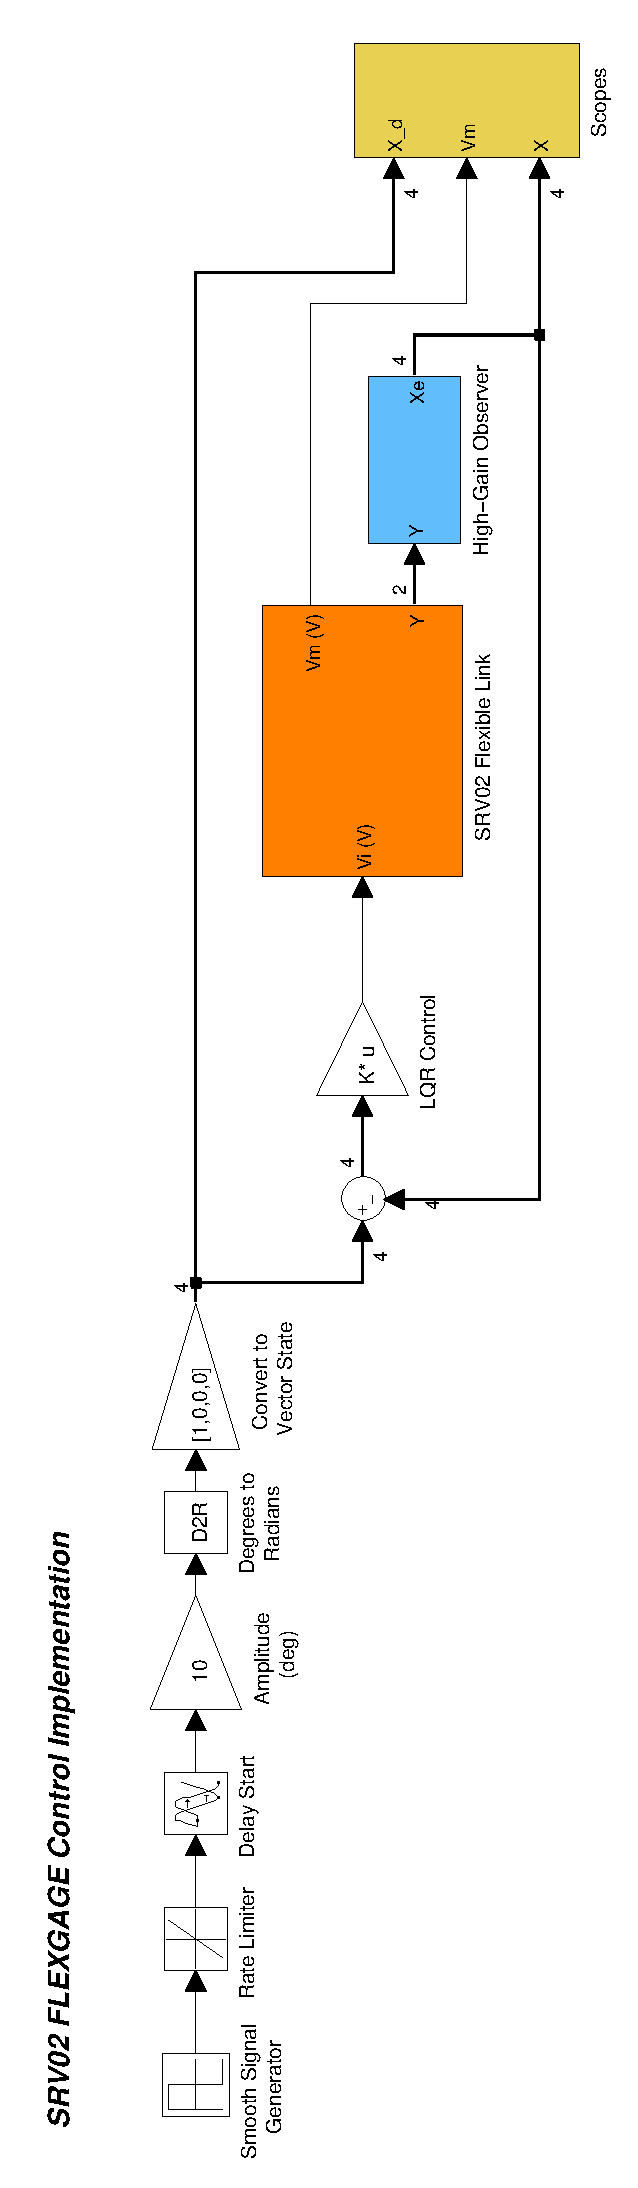
\includegraphics[width=0.3\linewidth,angle=-90]{eps/lab_4/lqr_simulink}
    \caption{A Simulink model that inputs a signal into the rotary flexible beam system and observes its output. This model can be used to drive the rotor base to track a signal input while minimizing the flexible beam deflections via full state feedback. The feedback gain $K$ is designed using a linear quadratic regulator.}
    \label{lab4_lqr_simulink}
\end{figure}

Your first task will be to observe the effects of changing the diagonal weightings of $Q$. Using your state-space matrices from \hyperref[subsection:lab4_prelab]{Section~\ref{subsection:lab4_prelab}}, and setting
\[
    Q = \left[\begin{array}{c c c c}
            q_1 & 0   & 0   & 0   \\
            0   & q_2 & 0   & 0   \\
            0   & 0   & q_3 & 0   \\
            0   & 0   & 0   & q_4
        \end{array}\right]
\]
you can use the MATLAB command \emph{care} to solve the continuous algebraic Ricatti equation (CARE). This will return the solutions to the Riccati equation, $\Pi_{\infty}$, which you will use to compute your feedback gain, $K=-B^T \Pi_{\infty}$.
\begin{enumerate}
    \item[Q2:] Using a diagonal weightings matrix for $Q$, express the cost function symbolically. What would be the effect of increasing the diagonal elements $q_i$ on the feedback gain, $K$?\\
          \drew{Answer:
              \begin{align*}
                  \eta(u) & = \bigint_0^{\infty} \left( [\theta \quad \alpha \quad \dot{\theta} \quad \dot{\alpha}] \left[\begin{array}{c c c c}
                          q_1 & 0   & 0   & 0   \\
                          0   & q_2 & 0   & 0   \\
                          0   & 0   & q_3 & 0   \\
                          0   & 0   & 0   & q_4
                      \end{array}\right] \left[\begin{array}{c} \theta \\ \alpha \\ \dot{\theta} \\ \dot{\alpha} \end{array}\right] + u^T(t)u(t) \right)\; dt \\
                          & = \int_0^{\infty} q_1\theta^2 + q_2\alpha^2 + q_3\dot{\theta}^2 + q_4\dot{\alpha}^2 +u^2(t) \; dt
              \end{align*}
              Increasing the weightings $q_i$ would alter the cost function so as to give the corresponding state more influence over the cost, e.g., increasing $q_1$ would cause the control input $u(t)$ to have a bias towards minimizing the state scaled by $q_1$ (in our lab, this state is $\theta$), and thus would increase the corresponding feedback gain element $k_1$ to compensate, where
              \[
                  K = \left[\begin{array}{c} k_1 \\ k_2 \\ k_3 \\ k_4 \end{array}\right].
              \]
              This behaviour is the same for all weightings $q_i$. Note that due to the interconnectedness of the system states, changing one $q_i$ may (and usually will) effect multiple states.
          }
    \item[Q3:] \emph{Check your feedback gain with your TA}. Since the Simulink model \emph{subtracts} the feedback from the input, make sure you define $K$ as $K=B^T \Pi_{\infty}$ and \textbf{not} $-K=B^T \Pi_{\infty}$. Vary the weightings $q_1,\; q_2,\; q_3,\; q_4$ independently from starting values $[q_1,\; q_2,\; q_3,\; q_4] = [1,\; 1,\; 1,\; 1]$. Run \textbf{lqr\_model.mdl} with a square wave input of amplitude 30 \textbf{total} (there is a signal amplitude \& an amplitude block, multiply these to get 30) and with frequency of 0.33 Hz. What effects does each modification have on the feedback gain, $K = [k_1,\; k_2,\; k_3,\; k_4]$? Plot each of the state responses with respect to time. What effects does each modification have on the physical system's state responses? What weighting(s) has(have) noticeable effects on reducing the rise time (one in particular is noticeable)? Did any decrease the flexible beam's deflections? \emph{Formulate problems and their specifications} that you anticipate when tuning particular weightings in various \emph{engineering applications} (e.g., for tidal power generators - or flexible beams mounted on the ocean floor in locations of notably strong tidal power - where the flexible beam's deflections trigger a power generator, but can also be strained to failure).\\
          \drew{Answer: Here are the plots and the corresponding feedback gains produced by the linear quadratic regulator:
              \begin{figure}[htb!]
                  \subfigure{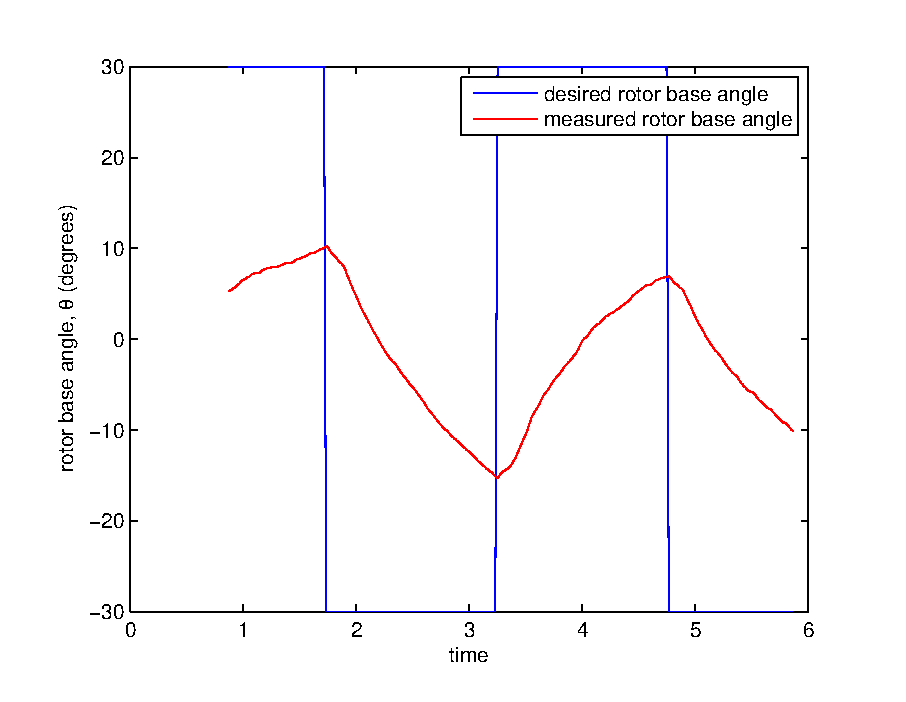
\includegraphics[width=0.5\linewidth]{eps/lab_4/theta_q_1_1_1_1}}
                  \subfigure{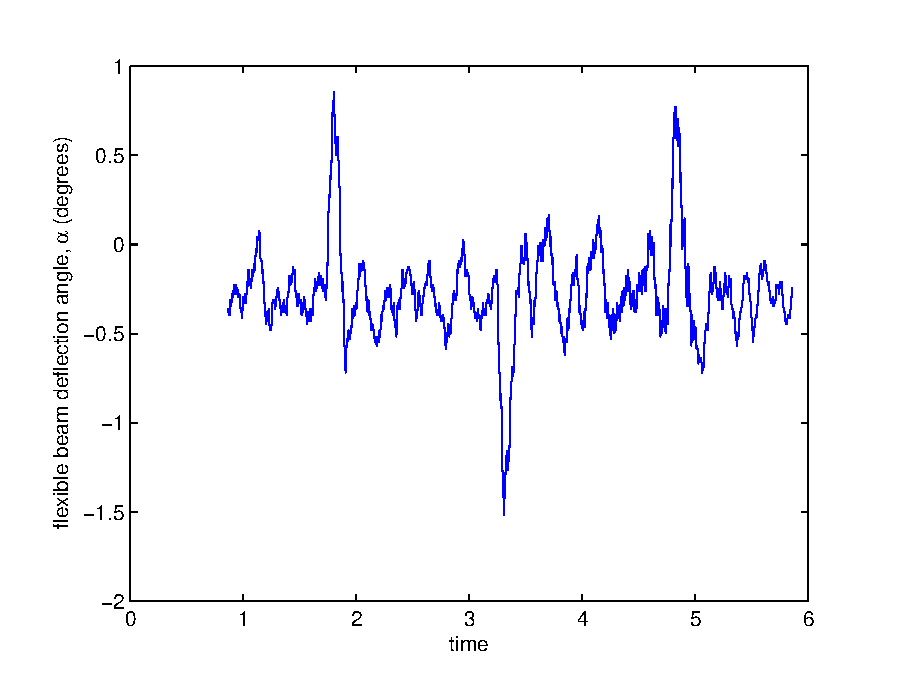
\includegraphics[width=0.5\linewidth]{eps/lab_4/alpha_q_1_1_1_1}}
                  \caption{a) The rotor base response to a square wave input when $[q_1,\; q_2,\; q_3,\; q_4] = [1,\; 1,\; 1,\; 1]$, giving $[k_1,\; k_2,\; k_3,\; k_4] = [1,\; -9.5873,\; 0.6004,\; -0.4092]$, and b) the corresponding flexible beam deflection angle with respect to time.}
              \end{figure}
              \begin{figure}[htb!]
                  \subfigure{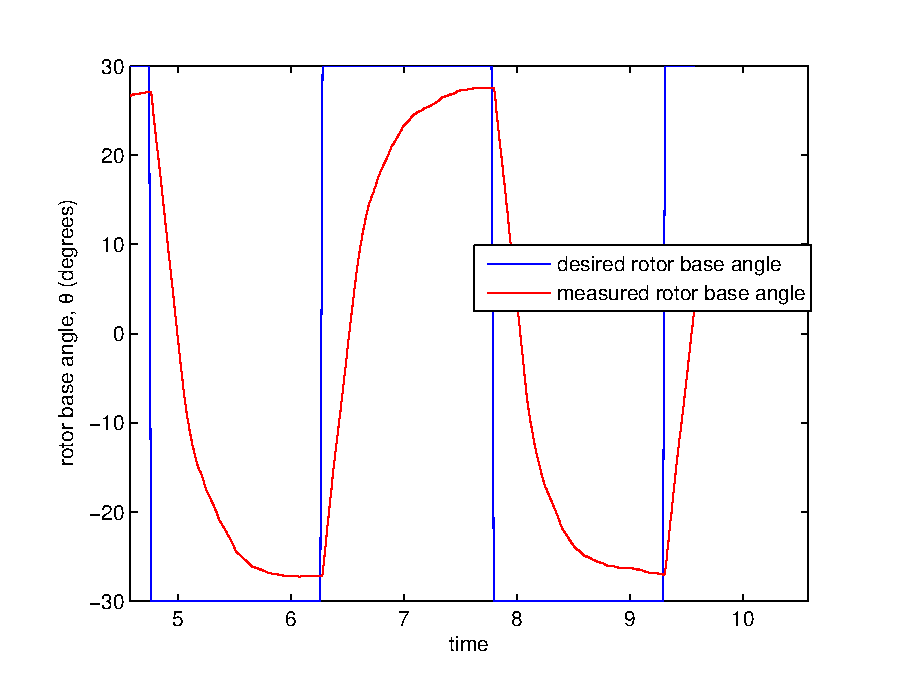
\includegraphics[width=0.5\linewidth]{eps/lab_4/theta_q_20_1_1_1}}
                  \subfigure{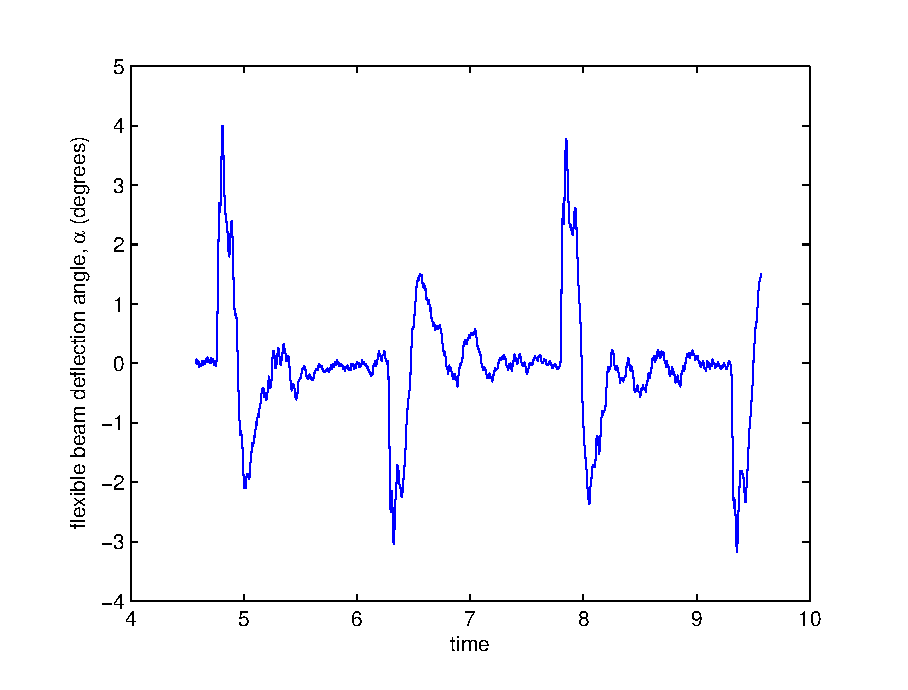
\includegraphics[width=0.5\linewidth]{eps/lab_4/alpha_q_20_1_1_1}}
                  \caption{a) The rotor base response to a square wave input when $[q_1,\; q_2,\; q_3,\; q_4] = [20,\; 1,\; 1,\; 1]$, giving $[k_1,\; k_2,\; k_3,\; k_4] = [4.4721,\; -10.464,\; 0.798,\; -0.253]$, and b) the corresponding flexible beam deflection angle with respect to time.}
              \end{figure}
              \begin{figure}[htb!]
                  \subfigure{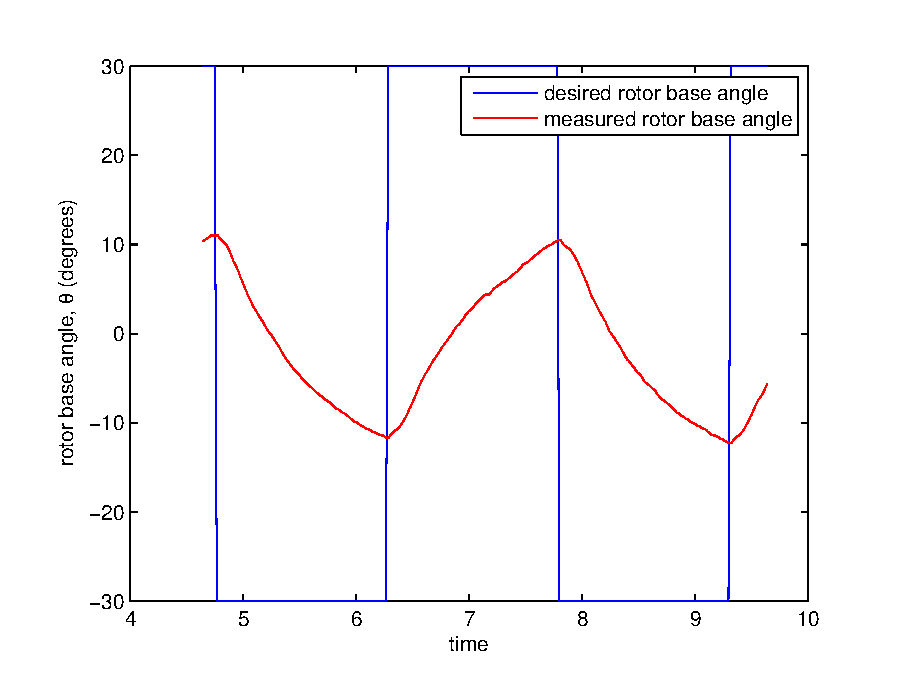
\includegraphics[width=0.5\linewidth]{eps/lab_4/theta_q_1_20_1_1}}
                  \subfigure{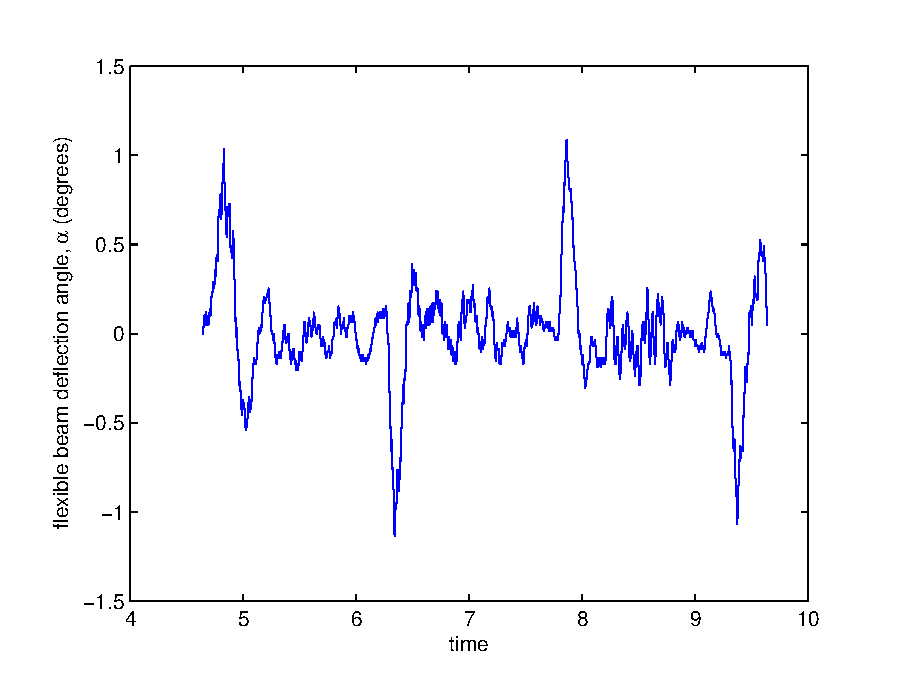
\includegraphics[width=0.5\linewidth]{eps/lab_4/alpha_q_1_20_1_1}}
                  \caption{a) The rotor base response to a square wave input when $[q_1,\; q_2,\; q_3,\; q_4] = [1,\; 20,\; 1,\; 1]$, giving $[k_1,\; k_2,\; k_3,\; k_4] = [1,\; -10.408,\; 0.601,\; -0.413]$, and b) the corresponding flexible beam deflection angle with respect to time.}
              \end{figure}
              \begin{figure}[htb!]
                  \subfigure{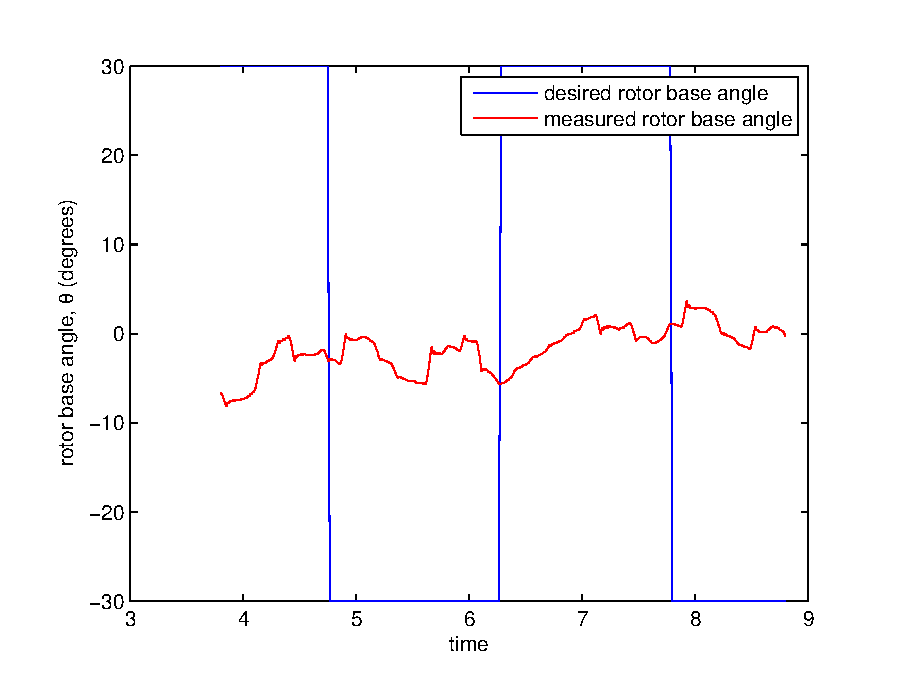
\includegraphics[width=0.5\linewidth]{eps/lab_4/theta_q_1_1_20_1}}
                  \subfigure{\includegraphics[width=0.5\linewidth]{eps/lab_4/alpha_q_1_1_20_1}}
                  \caption{a) The rotor base response to a square wave input when $[q_1,\; q_2,\; q_3,\; q_4] = [1,\; 1,\; 20,\; 1]$, giving $[k_1,\; k_2,\; k_3,\; k_4] = [1,\; -10.85,\; 3.881,\; -0.133]$, and b) the corresponding flexible beam deflection angle with respect to time.}
              \end{figure}
              \begin{figure}[htb!]
                  \subfigure{\includegraphics[width=0.5\linewidth]{eps/lab_4/theta_q_1_1_1_20}}
                  \subfigure{\includegraphics[width=0.5\linewidth]{eps/lab_4/alpha_q_1_1_1_20}}
                  \caption{a) The rotor base response to a square wave input when $[q_1,\; q_2,\; q_3,\; q_4] = [1,\; 1,\; 1,\; 20]$, giving $[k_1,\; k_2,\; k_3,\; k_4] = [1,\; -43.48,\; 0.677,\; -3.449]$, and b) the corresponding flexible beam deflection angle with respect to time.}
              \end{figure}}

          \clearpage
          \drew{One will notice that increasing $q_1$ has an impact on changing $k_1$, and that the rotor base response is much faster (rise time and settling time is decreased). Also, increasing $q_4$ has a large impact on changing $k_4$, and thus from a theoretical standpoint, the angular velocity of the flexible beam should be reduced by increasing $q_4$. The other weightings, $q_2$ and $q_3$, have little effect on the system.
          }
    \item[Q4:] You will perform a similar experiment with the same input (square wave with amplitude of 30 and frequency of 0.33$Hz$), except now there are \emph{design restrictions} on the rotor base's response: we require that maximum percent overshoot to be 10\%, the rise time be within 0.5 seconds and the steady-state error be within 5\% for use in our application. In addition, the maximum flexible beam deflection should be no more than 10\degree. Tune the diagonal weightings of $Q$ until you've achieved the desired results, and then plot the rotor's base angle, $\theta$, and the flexible beam's deflection angle, $\alpha$, with respect to time. Also plot the control input with respect to time. What weightings in the matrix $Q$ did you use to achieve these results, and what was the resulting feedback gain, $K$?\\
          \drew{Answer: The weightings that were used to achieve the desired performance was $[q_1,\; q_2,\; q_3,\; q_4] = [130,\; 1,\; 1,\; 3.5]$, giving $[k_1,\; k_2,\; k_3,\; k_4] = [11.401,\; -25.031,\; 1.379,\; -0.436]$. Instructors should note that there can be large variances between flexible beam modules, so these answers should be marked correct not by whether students can replicate the same weightings but by whether they can achieve that achieve the required response characteristics. Here are the plots:
          \begin{figure}[htb!]
              \center{
                  \subfigure{\includegraphics[width=0.4\linewidth]{eps/lab_4/theta_q_130_1_1_3half}}
                  \subfigure{\includegraphics[width=0.4\linewidth]{eps/lab_4/alpha_q_130_1_1_3half}}
                  \subfigure{\includegraphics[width=0.4\linewidth]{eps/lab_4/vm_q_130_1_1_3half}}}
              \caption{a) The rotor base angle, and (b) the flexible beam deflection angle responses to a square wave input, with matrix $Q$ tuned to achieve the desired performance metrics.}
          \end{figure}
          }
\end{enumerate}
\newpage
\subsection{Effects of Partial State Feedback on LQR}\label{subsubsection:lab4_partial_feedback}
Now, you will observe the effects of using only partial state feedback in your closed-loop system on the optimality of the control system. Open the Simulink model\\ \textbf{lqr\_partial\_feedback\_model.mdl}. Notice that the only state feedback being used is $\theta$ and the high-gain observer estimate of $\dot{\theta}$, as shown in Figure~\ref{lab4_lqr_partial_simulink}.
\begin{figure}[htb!]
    \includegraphics[width=0.3\linewidth,angle=-90]{eps/lab_4/lqr_partial_feedback_simulink}
    \caption{A Simulink model of the rotary flexible beam that utilizes partial state feedback and the linear quadratic regulator to design a feedback gain, $K$, that minimizes the deflections of the flexible beam while the rotor base tracks a square wave trajectory.}
    \label{lab4_lqr_partial_simulink}
\end{figure}

\begin{enumerate}
    \item[Q5:] Similar to the last experiment, use the LQR technique and the same weighting matrix $Q$ when computing your feedback gain, $K$. Plot the system responses to a square wave function with amplitude 30 and with frequency of 0.33 Hz. Compare the optimality of full state feedback and the partial state feedback closed-loop systems. Describe at least two previously-learned techniques that you may employ (and describe how) to obtain a better state feedback design, leading to superior system behaviour.\\
          \drew{Answer: in the partial state feedback case, the closed-loop control system is less optimal than the full state feedback system: the beam deflects much more and the steady-state error is higher. Due to the design of the cost function, these increases in beam deflection and steady-state error result in a higher cost. The control input is slightly less, but due to the design of the cost function, this will lower the cost significantly.
              \begin{figure}[htb!]
                  \subfigure{\includegraphics[width=0.48\linewidth]{eps/lab_4/theta_q_130_1_1_3half_partial}}
                  \subfigure{\includegraphics[width=0.5\linewidth]{eps/lab_4/alpha_q_130_1_1_3half_partial}}
                  \center{
                      \subfigure{\includegraphics[width=0.5\linewidth]{eps/lab_4/vm_q_130_1_1_3half_partial}}}
                  \caption{a) The rotor base angle, and (b) the flexible beam deflection angle responses to a square wave input when using only partial state feedback. This partial state feedback control system is less optimal than the full state feedback control system.}
              \end{figure}
          }
\end{enumerate}
\newpage

\subsection{Designing an Observer \& Using Observer Estimate as Feedback for LQ Problem}\label{subsection:lab4_observer_lqr}
\begin{enumerate}
    \item[Q6:] Is it possible to construct an observer for the rotary flexible link system, for the scenario where the strain gauge, which reads the flexible beam's deflection angle, is damaged?\\
          \drew{Answer: with this modification, the state-space matrix $C$ becomes
              \[
                  C = \left[\begin{array}{c c c c}
                          1 & 0 & 0 & 0 \\
                          0 & 0 & 0 & 0
                      \end{array}\right]
              \]
              and the observability matrix becomes
              \[
                  \mathcal{O}_{(A,C)} = \left[\begin{array}{c c c c}
                          1 & 0         & 0       & 0      \\
                          0 & 0         & 0       & 0      \\
                          0 & 0         & 1       & 0      \\
                          0 & 0         & 0       & 0      \\
                          0 & 623.77    & -40.49  & 0      \\
                          0 & 0         & 0       & 0      \\
                          0 & -25257.84 & 1639.61 & 623.77 \\
                          0 & 0         & 0       & 0
                      \end{array}\right]
              \]
              which has full rank. The controllability matrix does not change. Thus the modified system is controllable and observable, which implies that it is detectable and stabilizable. Hence, one can hope to construct an observer for the state $\alpha$, and then use the high-gain observer subsystem block to estimate $\dot{\alpha}$.}
\end{enumerate}
\begin{figure}[htb!]
    \centering
    \includegraphics[width=0.6\linewidth,angle=-90]{eps/lab_4/lqr_observer_model}
    \caption{A Simulink subsystem block showing the rotary pendulum system and a Luenberger observer. These systems are not connected, however one can connect these in such a way to compare the measured and estimated pendulum angle, $\alpha$ and $\hat{\alpha}$, as well as use the pendulum angle estimate as LQR feedback. Note that this model will not run without modification.}
    \label{figure:lab4_lqr_observer_model}
\end{figure}
\newpage
\begin{enumerate}
    \item[Q7:] Open the Simulink model \textbf{lqr\_observer\_model} with the Luenberger observer contained in the rotary pendulum's subsystem block, as shown in Figure~\ref{figure:lab4_lqr_observer_model}. Follow the procedure from \hyperref[subsection:lab3_observer]{Section~\ref{subsection:lab3_observer}} of Lab 3 to build a Luenberger state observer to estimate state $\alpha$. You will need to tune your observer gain, $L$, similarly to how you did so in Lab 3 so that the observer dynamics are faster than the system dynamics. However, now your feedback gain $K$ is being produced by the linear quadratic regulator, so tuning $Q$ will alter $K$ and thus the observer gain $L$ may have to be tuned concurrently. \textbf{Make sure} to change your output matrix, $C$, such that $\alpha$ is not an output. Use the estimate of the beam's deflection angle, $\hat{\alpha}$, to calculate an estimate for the angular velocity of the beam via the high-gain observer subsystem. Plot the responses of the rotor base angle and the flexible beam deflection angle due to a square wave input of amplitude 30 and frequency 0.33Hz. On the flexible beam deflection angle plot, also plot your state estimate (you'll need to use a To Workspace block for this). What are your gains $L$ and $K$ and what is your weighting matrix $Q$? What can you conclude about the optimality (i.e., rotor base trajectory tracking and beam's deflections) of this control system when comparing it to the partial state feedback scenario and the full state feedback scenario?\\
          \drew{Answer: with $Q$ weightings of $[q_1,\; q_2,\; q_3,\; q_4] = [130,\; 1,\; 1,\; 3.5]$, the resulting feedback gain weightings are $[k_1,\; k_2,\; k_3,\; k_4] = [11.401,\; -25.031,\; 1.379,\; -0.436]$. The observer gain weightings are $[l_1,\; l_2,\; l_3,\; l_4] = [-40,\; -41,\; -42,\; -43]$. The plots below reveal that the state estimate, $\hat{\alpha}$, and $\alpha$ agree pretty well. As a result of using partial state feedback and state estimate feedback, the magnitude of the flexible beam deflections is reduced throughout in comparison to the partial state feedback closed-loop system. In comparison to the full state feedback system, the overall flexible beam deflections are greater, and the rotor angle response is almost the same. The control input for the state estimate feedback system is slightly less than that for the full state feedback system, although this decrease is only weighted by 1 in the cost function, whereas beam deflection is weighted by 3.5. Thus using the state estimates as feedback is a more optimal control system than using only partial feedback, but not as optimal as using full state feedback (as is expected).
          \begin{figure}[htb!]
              \subfigure{\includegraphics[width=0.5\linewidth]{eps/lab_4/theta_observer_feedback}}
              \subfigure{\includegraphics[width=0.5\linewidth]{eps/lab_4/alpha_observer_feedback}}
              \center{
                  \subfigure{\includegraphics[width=0.5\linewidth]{eps/lab_4/vm_observer_feedback}}
                  \caption{a) The rotor base angle, and (b) the flexible beam deflection angle responses to a square wave input when using partial state feedback $\theta$, $\dot{\theta}$ and state estimate feedback, $\hat{\alpha}$, $\hat{\dot{\alpha}}$. This control system is less optimal than the full state feedback control system, but more optimal than the partial state feedback system.}}
          \end{figure}
          }
\end{enumerate}

\newpage
\subsection{Deliverables}
To recap the lab objectives, this is what you need to include in your lab report to obtain full marks:
\begin{enumerate}
    \item prelab question (i) and (ii);
    \item the answers to questions Q3, Q4, Q5 and Q7 (include plots where requested).
\end{enumerate}
\textbf{Note:} Congratulations on finishing your MTHE 430 labs! Celebrations are in order.


\bibliographystyle{ieeetr}%
\bibliography{DS}
\end{document}